\documentclass[lang=cn,10pt,scheme=chinese,toc=twocol]{elegantbook}
\usepackage{float}
\usepackage{amsmath}
\usepackage{tikz}
\usetikzlibrary{quotes,angles}
\usepackage{wrapfig}
\numberwithin{figure}{section}
\numberwithin{table}{section}
\newcommand{\arccot}{\mathrm{arccot}\,}
\newcommand{\deriv}{\mathrm{d}}
\newcommand{\pll}{\hspace{0.7ex}
\begin{tikzpicture}[line width = 0.08 ex, line cap = round]
\draw (0, 0) -- (0.55ex, 1.5ex); % 倾斜角度为70度
\draw[xshift=0.6ex] (0, 0) -- (0.55ex, 1.5ex);
\end{tikzpicture}\hspace{0.6ex}
} % 平行
\usepackage{newtxmath}
\usepackage{bm}

\title{高等数学章节总结}
% \subtitle{Elegant\LaTeX{} 经典之作}

% \author{Ethan Deng \& Liam Huang}
\institute{数学协会}
% \date{April 9, 2022}
% \version{4.3}
% \bioinfo{自定义}{信息}

\extrainfo{世界上最远的距离,是我说$Q^\text{T}AQ$,你却以为我在卖萌}

% 修改标题页的橙色带
\definecolor{customcolor}{RGB}{32,178,170}
\colorlet{coverlinecolor}{customcolor}

\setcounter{tocdepth}{3}

\logo{logo.jpeg}
\cover{cover.png}

% 本文档命令
\usepackage{array}
\newcommand{\ccr}[1]{\makecell{{\color{#1}\rule{1cm}{1cm}}}}

\begin{document}
    \maketitle
    \frontmatter
    
    \tableofcontents
    
    \mainmatter
    
    \chapter*{关于数学协会与本书内容}
    天津工业大学数学协会成立于1998年6月1日,登记注册的社员近150人,作为最为传统的协会之一,我们立足于基础数学学科,面向全校的数学爱好者,秉持相互交流学习数学的初心来提高同学们学习数学的兴趣和能力。同时,我们通过举办讲座、在线答疑、在线解题等活动增进并创造良好的学习氛围,定期在协会群和教室里交流思想,发散思维,由此激发同学们的学习兴趣。

    本书内容基于同济第八版《高等数学》进行提炼总结,适用于同学们在学习完相应内容后复习使用,作为预习的内容相对简略且不易懂,建议优先观看对应的课程或者教材。
    带星号(*)部分为竞赛进阶内容,扩充书上及相关习题册部分未讲解的内容,仅应对期末考试的同学可以不要求掌握。

    本书采用ElegantBook模板编写,详细LaTeX代码详见GitHub仓库:https://github.com/MorningKay/Calculus-Note

    \chapter*{基础知识补充}
\addcontentsline{toc}{chapter}{基础知识补充}
\markboth{基础知识补充}{基础知识补充}

\section{三角函数}
\subsection{三角函数图像及性质}
\textbf{正切函数与余切函数}

正切函数$y=\tan x$(见图\ref{tan}),余切函数$y=\cot x$(见图\ref{cot})
\begin{figure}[H]
\centering
\begin{minipage}{0.4\linewidth}
    \centerline{\includegraphics[width=\textwidth]{figure/tan_plot.png}}
    \caption{} \label{tan}
\end{minipage}
    \qquad
\begin{minipage}{0.4\linewidth}
    %\vspace{3pt}
    \centerline{\includegraphics[width=\textwidth]{figure/cot_plot.png}}
    \caption{} \label{cot}
\end{minipage}
\end{figure}

\begin{note}
    \begin{enumerate}
        \item 定义域:$y=\tan x$的定义域为$x\neq k\pi+\dfrac{\pi}{2}(k\in Z)$的一切实数$x$;
        \vspace{2mm}

        $y=\cot x$的定义域为$x\neq k\pi(k\in Z)$的一切实数$x$。

        值域:$(-\infty,+\infty)$

        \item 奇偶性:$y=\tan x$和$y=\cot x$均为奇函数(在其定义域内)。

        \item 周期性:$y=\tan x$和$y=\cot x$均以$\pi$为最小正周期(在其定义域内)。
    \end{enumerate}
\end{note}
~\\

\textbf{正割函数与余割函数}

正割函数$y=\sec x$(见图\ref{sec}),余割函数$y=\csc x$(见图\ref{csc})
\begin{equation}
    \sec x = \dfrac{1}{\cos x}, \quad \csc x = \dfrac{1}{\sin x} \nonumber
\end{equation}

\begin{figure}[H]
\centering
\begin{minipage}{0.4\linewidth}
    \centerline{\includegraphics[width=\textwidth]{figure/sec_plot.png}}
    \caption{} \label{sec}
\end{minipage}
    \qquad
\begin{minipage}{0.4\linewidth}
    %\vspace{3pt}
    \centerline{\includegraphics[width=\textwidth]{figure/csc_plot.png}}
    \caption{} \label{csc}
\end{minipage}
\end{figure}

\begin{note}
    \begin{enumerate}
        \item 定义域:$y=\sec x$的定义域为$x\neq k\pi+\dfrac{\pi}{2}(k\in Z)$的一切实数$x$;
        \vspace{2mm}

        $y=\csc x$的定义域为$x\neq k\pi(k\in Z)$的一切实数$x$。

        值域:$(-\infty,-1]\cup [1,+\infty)$

        \item 奇偶性:$y=\sec x$为偶函数,$y=\csc x$为奇函数(在其定义域内)。

        \item 周期性:$y=\sec x$和$y=\csc x$均以$2\pi$为最小正周期(在其定义域内)。
    \end{enumerate}
\end{note}

\subsection{反三角函数函数图像及性质}
\textbf{反正弦函数与反余弦函数}

反正弦函数$y=\arcsin x$(见图\ref{arcsin}),反余弦函数$y=\arccos x$(见图\ref{arccos})
\begin{figure}[H]
\centering
\begin{minipage}{0.4\linewidth}
    \centerline{\includegraphics[width=\textwidth]{figure/arcsin_plot.png}}
    \caption{} \label{arcsin}
\end{minipage}
    \qquad
\begin{minipage}{0.4\linewidth}
    %\vspace{3pt}
    \centerline{\includegraphics[width=\textwidth]{figure/arccos_plot.png}}
    \caption{} \label{arccos}
\end{minipage}
\end{figure}

$y=\arcsin x$是$y=\sin x\left(-\dfrac{\pi}{2}\leq x\leq \dfrac{\pi}{2}\right)$的反函数,$y=\arccos x$是$y=\cos x(0\leq x\leq \pi)$的反函数

\begin{note}
    \begin{enumerate}
        \item 定义域:[-1,1]

        值域:$y=\arcsin x$的值域为$\left[-\dfrac{\pi}{2},\dfrac{\pi}{2}\right]$,$y=\arccos x$的值域为$[0,\pi]$。

        \item 单调性:$y=\arcsin x$单调增加,$y=\arccos x$单调减少。

        \item 奇偶性:$y=\arcsin x$为奇函数(在其定义域内)。

        \item 有界性:两个函数在其定义域内有界,$-\dfrac{\pi}{2}\leq \arcsin x\leq \dfrac{\pi}{2}, 0\leq \arccos x\leq\pi$

        \item 性质:$\arcsin x+\arccos x = \dfrac{\pi}{2}(-1\leq x \leq 1)$
        \begin{proof}
            令$f(x)=\arcsin x+\arccos x,-1\leq x \leq 1$,则$f'(x)=\dfrac{1}{\sqrt{1-x^2}}-\dfrac{1}{\sqrt{1-x^2}}=0$,于是$f(x)=C$(常数),又$f(0)=\dfrac{\pi}{2}$,故$f(x)=\dfrac{\pi}{2}$,证毕。
        \end{proof}

        \item 特殊函数值:
        \begin{equation}
        \begin{aligned}
            &
            \arcsin 0 = 0, \quad \arcsin \dfrac{1}{2} = \dfrac{\pi}{6}, \quad \arcsin \dfrac{\sqrt{2}}{2} = \dfrac{\pi}{4}, \quad \arcsin \dfrac{\sqrt{3}}{2} = \dfrac{\pi}{3}, \quad \arcsin 1 = \dfrac{\pi}{2} \\
            &
            \arccos 1 = 0, \quad \arccos \dfrac{\sqrt{3}}{2} = \dfrac{\pi}{6}, \quad \arccos \dfrac{\sqrt{2}}{2} = \dfrac{\pi}{4}, \quad \arccos \dfrac{1}{2} = \dfrac{\pi}{3}, \quad \arccos 0 = \dfrac{\pi}{2}
        \end{aligned}    \nonumber
        \end{equation}
    \end{enumerate}
\end{note}
~\\

\textbf{反正切函数与反余切函数}

反正弦函数$y=\arctan x$(见图\ref{arctan}),反余弦函数$y=\arccot x$(见图\ref{arccot})
\begin{figure}[H]
\centering
\begin{minipage}{0.4\linewidth}
    \centerline{\includegraphics[width=\textwidth]{figure/arctan_plot.png}}
    \caption{} \label{arctan}
\end{minipage}
    \qquad
\begin{minipage}{0.4\linewidth}
    %\vspace{3pt}
    \centerline{\includegraphics[width=\textwidth]{figure/arccot_plot.png}}
    \caption{} \label{arccot}
\end{minipage}
\end{figure}

$y=\arctan x$是$y=\tan x\left(-\dfrac{\pi}{2}< x< \dfrac{\pi}{2}\right)$的反函数,$y=\arccot x$是$y=\cot x(0< x< \pi)$的反函数

\begin{note}
    \begin{enumerate}
        \item 定义域:$(-\infty,+\infty)$

        值域:$y=\arctan x$的值域为$\left(-\dfrac{\pi}{2},\dfrac{\pi}{2}\right)$,$y=\arccot x$的值域为$(0,\pi)$。

        \item 单调性:$y=\arctan x$单调增加,$y=\arccot x$单调减少。

        \item 奇偶性:$y=\arctan x$为奇函数(在其定义域内)。

        \item 有界性:两个函数在其定义域内有界,$-\dfrac{\pi}{2}< \arctan x< \dfrac{\pi}{2}, 0< \arccot x<\pi$

        \item 性质:$\arctan x+\arccot x = \dfrac{\pi}{2}(-\infty< x <\infty)$
        \begin{proof}
            令$f(x)=\arctan x+\arccot x,-\infty< x <\infty$,则$f'(x)=\dfrac{1}{1+x^2}-\dfrac{1}{1+x^2}=0$,于是$f(x)=C$(常数),又$f(0)=\dfrac{\pi}{2}$,故$f(x)=\dfrac{\pi}{2}$,证毕。
        \end{proof}
        \vspace{2mm}

        \item 特殊函数值:
        \begin{equation}
        \begin{aligned}
            &
            \arctan 0 = 0, \quad \arctan \dfrac{\sqrt{3}}{3} = \dfrac{\pi}{6}, \quad \arctan 1 = \dfrac{\pi}{4}, \quad \arctan \sqrt{3} = \dfrac{\pi}{3} \\
            &
            \arccot 0 = \dfrac{\pi}{2}, \quad \arccot \sqrt{3} = \dfrac{\pi}{6}, \quad \arccot 1 = \dfrac{\pi}{4}, \quad \arccot \dfrac{\sqrt{3}}{3} = \dfrac{\pi}{3}
        \end{aligned}    \nonumber
        \end{equation}

        \item 极限:$\displaystyle \lim_{x\rightarrow -\infty} \arctan x = -\dfrac{\pi}{2}, \quad \lim_{x\rightarrow +\infty} \arctan x = \dfrac{\pi}{2}, \quad \lim_{x\rightarrow-\infty} \arccot x = \pi, \quad \lim_{x\rightarrow +\infty} \arccot x = 0$
    \end{enumerate}
\end{note}

\subsection{三角函数公式}
\textbf{三角函数基本关系}
\begin{equation}
    \begin{aligned}
        &\sin^2\alpha + \cos^2\alpha = 1 \\
        &1 + \tan^2\alpha = \sec^2\alpha \\
        &1 + \cot^2\alpha = \csc^2\alpha
    \end{aligned}\nonumber
\end{equation}

\textbf{倍角公式}
\begin{equation}
    \begin{aligned}
        & \sin 2\alpha = 2\sin\alpha\cos\alpha, \quad \cos 2\alpha = \cos^2\alpha-\sin^2\alpha = 1 - 2\sin^2\alpha = 2\cos^2\alpha - 1 \\
        & \sin 3\alpha = -4\sin^3\alpha+3\sin\alpha, \quad \cos 3\alpha = 4\cos^3\alpha-3\cos\alpha \\
        & \tan 2\alpha = \dfrac{2\tan\alpha}{1-\tan^2\alpha}, \quad \cot 2\alpha = \dfrac{\cot^2\alpha-1}{2\cot\alpha}
    \end{aligned}\nonumber
\end{equation}

\textbf{半角公式}
\begin{equation}
    \begin{aligned}
        & \sin^2\dfrac{\alpha}{2} = \dfrac{1}{2}(1-\cos\alpha), \quad \cos^2\dfrac{\alpha}{2} = \dfrac{1}{2}(1+\cos\alpha) \\
        & \sin\dfrac{\alpha}{2} = \pm\sqrt{\dfrac{1-\cos\alpha}{2}}, \quad \cos\dfrac{\alpha}{2} = \pm\sqrt{\dfrac{1+\cos\alpha}{2}} \\
        & \tan\dfrac{\alpha}{2} = \dfrac{1-\cos\alpha}{\sin\alpha}=\dfrac{\sin\alpha}{1+\cos\alpha}=\pm\sqrt{\dfrac{1-\cos\alpha}{1+\cos\alpha}} \\ 
        & \cot\dfrac{\alpha}{2} = \dfrac{\sin\alpha}{1-\cos\alpha} = \dfrac{1+\cos\alpha}{\sin\alpha} = \pm\sqrt{\dfrac{1+\cos\alpha}{1-\cos\alpha}}
    \end{aligned} \nonumber
\end{equation}

\textbf{和差公式}
\begin{equation}
    \begin{aligned}
        &\sin(\alpha\pm\beta)=\sin\alpha\cos\beta\pm\cos\alpha\sin\beta, \quad \cos(\alpha\pm\beta)=\cos\alpha\cos\beta\mp\sin\alpha\sin\beta \\
        &\tan(\alpha\pm\beta)=\dfrac{\tan\alpha\pm\tan\beta}{1\mp\tan\alpha\tan\beta}, \quad \cot(\alpha\pm\beta)=\dfrac{\cot\alpha\cot\beta\mp 1}{\cot\beta\pm\cot\alpha}
    \end{aligned}\nonumber
\end{equation}

\textbf{积化和差公式}
\begin{equation}
    \begin{aligned}
        &\sin\alpha\cos\beta = \dfrac{1}{2}[\sin(\alpha+\beta)+\sin(\alpha-\beta)], \quad \cos\alpha\sin\beta = \dfrac{1}{2}[\sin(\alpha+\beta)-\sin(\alpha-\beta)] \\
        &\cos\alpha\cos\beta = \dfrac{1}{2}[\cos(\alpha+\beta)+\cos(\alpha-\beta)], \quad \sin\alpha\sin\beta = \dfrac{1}{2} [\cos(\alpha-\beta)-\cos(\alpha+\beta)]
    \end{aligned} \nonumber
\end{equation}

\textbf{和差化积公式}
\begin{equation}
    \begin{aligned}
        &\sin\alpha+\sin\beta = 2\sin\dfrac{\alpha+\beta}{2}\cos\dfrac{\alpha-\beta}{2}, \quad \sin\alpha-\sin\beta=2\sin\dfrac{\alpha-\beta}{2}\cos\dfrac{\alpha+\beta}{2} \\
        &\cos\alpha+\cos\beta = 2\cos\dfrac{\alpha+\beta}{2}\cos\dfrac{\alpha-\beta}{2}, \quad \cos\alpha-\cos\beta=-2\sin\dfrac{\alpha+\beta}{2}\sin\dfrac{\alpha-\beta}{2}
    \end{aligned}\nonumber
\end{equation}

\textbf{万能公式}

若$u=\tan\dfrac{x}{2}(-\pi<x<\pi)$,则$\sin x=\dfrac{2u}{1+u^2}, \cos x=\dfrac{1-u^2}{1+u^2}$

\section{因式分解公式}
\begin{equation}
    \begin{aligned}
        &(a+b)^3=a^3+3a^2b+3ab^2+b^3, \quad (a-b)^3=a^3-3a^2b-3ab^2-b^3 \\
        &a^3-b^3=(a-b)(a^2+ab+b^2), \quad a^3+b^3=(a+b)(a^2-ab+b^2) \\
        &a^n-b^n=(a-b)(a^{n-1}+a^{n-2}b+\cdots+ab^{n-2}+b^{n-1})(n\mbox{是正整数}) \\
        &a^n-b^n=(a+b)(a^{n-1}-a^{n-2}b+\cdots-ab^{n-2}+b^{n-1})(n\mbox{为偶数}) \\
        &n\mbox{是正奇数时},a^n+b^n=(a+b)(a^{n-1}-a^{n-2}b+\cdots-ab^{n-2}+b^{n-1})
    \end{aligned} \nonumber \\
\end{equation}

\begin{equation}
    \begin{aligned}
        (a+b)^n=\sum_{k=0}^n\binom{n}{k}a^{n-k}b^k=
        &a^n+na^{n-1}b+\dfrac{n(n-1)}{2!}a^{n-2}b^2+\cdots+ \\
        &\dfrac{n(n-1)\cdots(n-k+1)}{k!}a^{n-k}b^k+\cdots+nab^{n-1}+b^n        
    \end{aligned}\nonumber
\end{equation}

\section{阶乘与双阶乘}
\begin{enumerate}
    \item $n!=1\cdot2\cdot3\cdot \ \cdots \ \cdot n$,规定$0!=1$。
    \item $(2n)!!=2\cdot4\cdot6\cdot \ \cdots \cdot (2n)=2^n\cdot n!$
    \item $(2n-1)!!=1\cdot3\cdot5\cdot \ \cdots \ \cdot (2n-1)$
\end{enumerate}

\section{常用不等式}
\begin{enumerate}
    \item 设$a,b$为实数,则(1)$\left|a\pm b\right|\leq\left|a\right|+\left|b\right|$;(2)$\left|\left|a\right|-\left|b\right|\right|\leq\left|a-b\right|$
    
    \item (1)$\sqrt{ab}\leq\dfrac{a+b}{2}\leq\sqrt{\dfrac{a^2+b^2}{2}} \quad (a,b>0)$ \\
    (2)$\sqrt[3]{abc}\leq\dfrac{a+b+c}{3}\leq\sqrt{\dfrac{a^2+b^2+c^3}{3}} \quad (a,b,c>0)$

    \item 若$0<a<x<b,0<c<y<d$,则$\dfrac{c}{b}<\dfrac{y}{x}<\dfrac{d}{a}$

    \item $\sin x<x< \tan x \quad \left( 0<x<\dfrac{\pi}{2} \right)$

    \item $\sin x<x \quad (x>0)$

    \item $\arctan x\leq x\leq \arcsin x \quad (0\leq x\leq 1)$

    \item $e^x\geq x+1 \quad (\forall x)$

    \item $x-1\geq\ln x \quad (x>0)$

    \item $\dfrac{1}{x+1}<\ln(1+\dfrac{1}{x})<\dfrac{1}{x} \quad (x>0)$
\end{enumerate}

    \chapter{函数与极限}

\begin{introduction}
    \item 函数的极限 \ref{def:function_limit}
    \item 极限存在定理 \ref{thm:squeeze_theorem_function}
    \item 无穷小的比较
    \item 介值定理 \ref{thm:the_intermediate_value_theorem}
    \item 数列的极限 \ref{def:sequence_limit}
    \item 单调数列定理 \ref{thm:monotonic_sequence_theorem}
\end{introduction}

\section{函数}
\subsection{函数的概念与性质}
设有两个变量$x$和$y$,如果变量$x$在其变化范围$D$内任取一个确定的数值时,变量$y$按照一定的规则$f$总有唯一确定的数值和它对应,则称变量$y$是变量$x$的函数,记为$y=f(x)$,$x$称为自变量,$y$称为因变量,$D$称为函数的定义域,$f$表示由$x$确定$y$的对应规则。

\begin{property} 函数的主要性质 \label{property:function}
\begin{enumerate}
\item 有界性 \quad 设函数$f(x)$在集合$D$上有定义,如果存在一个正常数$M$,使得对于$x$在$D$上的任意取值,均有$\left| f(x) \right|< M$,则称函数$f(x)$在$D$上有界,否则称函数$f(x)$在$D$上无界。

\item 单调性 \quad 设函数$f(x)$在某区间$D$上有定义,如果对于$D$上任意两点$x_1,x_2$,且$x_1< x_2$,均有$f(x_1)< f(x_2)$(或$f(x_1)> f(x_2)$),则称函数$f(x)$在$D$上单调增加(或单调减少),单调增加或单调减少函数统称为单调函数。

\item 奇偶性 \quad 设函数$f(x)$在关于原点对称的区间$D$上有定义,如果对$D$上任意点$x$,均有$f(-x)=f(x)$(或$f(-x)=-f(x)$),则称函数$f(x)$为偶函数(或奇函数)。

\item 周期性 \quad 设函数$f(x)$在集合$D$上有定义,如果存在正常数$T$,使得对于$D$上任意$x$,均有$f(x+T)=f(x)$,则称$f(x)$为周期函数,使上式成立的最小正数为周期函数的周期。
\end{enumerate}
\end{property}

\subsection{函数的极限}
\begin{definition}[函数的极限] \label{def:function_limit}
    设函数$f(x)$在点$x_0$的邻域内(点$x_0$可除外)有定义,$A$为一个常数,若对任意给定的$\varepsilon > 0$,都存在一个正数$\delta$,使得满足$0<\left|x-x_0\right|<\delta$的一切$x$所对应的$f(x)$都满足不等式$\left|f(x)-A\right|<\varepsilon$,则称$A$为函数$f(x)$当$x\rightarrow x_0$时的极限,记为
    \begin{equation}
        \lim_{x\rightarrow x_0} f(x)=A \nonumber
    \end{equation}

    若对于满足$0<x_0-x<\delta(0<x-x_0<\delta)$的一切$x$所对应的$f(x)$都满足不等式$\left|f(x)-A\right|<\varepsilon$,则称$A$为函数$f(x)$当$x$自$x_0$左(右)侧趋于$x_0$时的极限,即左(右)极限,分别记为
    \begin{equation}
        \lim_{x\rightarrow x_0^-} f(x) = f(x_0 -0) = A \quad (\lim_{x\rightarrow x_0^+} f(x) = f(x_0 +0) = A \ ) \nonumber
    \end{equation}

    类似地,可以给出当$x\rightarrow\infty,x\rightarrow +\infty, x\rightarrow -\infty$时,$f(x)$的极限为$A$的定义。
\end{definition}

\begin{property} 函数极限的性质 \label{property:function_limit}
    \begin{enumerate}
        \item 唯一性 \quad 若$\displaystyle\lim_{x\rightarrow x_0} f(x) = A$,则$A$必唯一。
        \item 有界性 \quad 若$\displaystyle\lim_{x\rightarrow x_0} f(x) = A$,则$f(x)$在$x_0$的某一邻域($x_0$除外)内是有界的。
        \item 保号性 \quad 设$f(x)$在$x_0$的某邻域($x_0$除外)内均有$f(x)\geq 0$(或$f(x)\leq 0$),且$\displaystyle\lim_{x\rightarrow x_0} f(x) = A$,则$A\geq 0$(或$A\leq 0$)。
    \end{enumerate}
\end{property}

\section{极限的运算}
\subsection{无穷小和无穷大}
\begin{definition}[无穷小与无穷大] \label{def:infty_and_zero}
    \begin{enumerate}
        \item 若$\displaystyle\lim_{x\rightarrow x_0 \atop (x\rightarrow \infty)} f(x) = 0$,则称$f(x)$当$x\rightarrow x_0(x\rightarrow\infty)$时为无穷小。
        
        \item 若对任意给定的$M>0$,都存在一个正数$\delta(N)$,使得满足$0<\left|x-x_0\right|<\delta(\left|x\right|>N)$的一切$x$所对应的$f(x)$都满足不等式$\left|f(x)\right|>M$,则称$f(x)$当$x\rightarrow x_0(x\rightarrow\infty)$时为无穷大,记为$\displaystyle\lim_{x\rightarrow x_0 \atop (x\rightarrow \infty)} f(x) = \infty$
    \end{enumerate}
\end{definition}

\textbf{无穷小和无穷大的关系}(以下所讨论的极限,都是在自变量同一变化过程中的极限)

\vspace{2mm}
若$\lim f(x) = 0 \quad (f(x)\neq 0)$,则$\lim \dfrac{1}{f(x)} = \infty$

\vspace{2mm}
若$\lim f(x) = \infty$,则$\lim \dfrac{1}{f(x)} = 0$

\subsection{运算法则}
\textbf{运算法则} \quad 设$\lim f(x)$和$\lim g(x)$均存在,则
\begin{flalign*}
    & \qquad\qquad\quad\lim \left[f(x)\pm g(x)\right]=\lim f(x)\pm \lim g(x) \\ 
    & \qquad\qquad\quad\lim \left[f(x)\cdot g(x)\right]=\lim f(x)\cdot \lim g(x) \\ 
    & \qquad\qquad\quad\lim \dfrac{f(x)}{g(x)} = \dfrac{\lim f(x)}{\lim g(x)} (\lim g(x)\neq 0) &
\end{flalign*}

\vspace{1mm}
\textbf{无穷小运算法则}
\begin{enumerate}
    \item 有限多个无穷小之和仍是无穷小。
    \item 有限多个无穷小之积仍是无穷小。
    \item 有界变量与无穷小之积仍为无穷小。
\end{enumerate}
\vspace{1mm}

\textbf{无穷小和函数极限的关系}

在一个极限过程中,函数$f(x)$的极限为$A$的充分必要条件是$f(x)=A+\alpha$,其中$\alpha$为这个极限过程中的无穷小量(即$\lim \alpha = 0$)

\section{极限存在定理 \quad 两个重要极限}
\begin{theorem}[夹逼定理] \label{thm:squeeze_theorem_function}
    设函数$f(x),g(x),h(x)$有定义,且满足以下条件:
    \begin{enumerate}
        \item 当$x\in \{ x \textbar \ 0 < \left|x-x_0\right| < h \}$或($\left|x\right|>M$)时,有$g(x)\leq f(x) \leq h(x)$成立。
        \item $\displaystyle \lim_{x\rightarrow x_0 \atop (x\rightarrow\infty)} g(x) = \lim_{x\rightarrow x_0 \atop (x\rightarrow\infty)} h(x) = a$,则$\displaystyle\lim_{x\rightarrow x_0 \atop (x\rightarrow\infty)} f(x)$存在,且$\displaystyle\lim_{x\rightarrow x_0 \atop (x\rightarrow\infty)} f(x) = a$
    \end{enumerate}
\end{theorem}

\begin{proof}
    假设$\varepsilon>0$,因为$\displaystyle\lim_{x\rightarrow x_0} g(x) = a$,存在一个数$\delta_1>0$
    \begin{equation}
        \mbox{如果} \qquad 0<\left|x - x_0\right| <\delta_1 \qquad \mbox{然后} \qquad \left|g(x) - a\right| < \varepsilon \nonumber
    \end{equation}

    即
    \begin{equation}
        \mbox{如果} \qquad 0<\left|x - x_0\right| <\delta_1 \qquad \mbox{然后} \qquad a-\varepsilon < g(x) < a+\varepsilon \nonumber
    \end{equation}

    因为$\displaystyle\lim_{x\rightarrow x_0} h(x) = a$,存在一个数$\delta_2>0$
    \begin{equation}
        \mbox{如果} \qquad 0<\left|x - x_0\right| <\delta_2 \qquad \mbox{然后} \qquad \left|h(x) - a\right| < \varepsilon \nonumber
    \end{equation}

    即
    \begin{equation}
        \mbox{如果} \qquad 0<\left|x - x_0\right| <\delta_2 \qquad \mbox{然后} \qquad a-\varepsilon < h(x) < a+\varepsilon \nonumber
    \end{equation}

    令$\delta = \min\{ \delta_1, \delta_2 \}$,如果$0<\left|x-x_0\right|<\delta$,则$0<\left|x-x_0\right|<\delta_1$和$0<\left|x-x_0\right|<\delta_2$,所以
    \begin{equation}
        a-\varepsilon<g(x)\leq f(x)\leq h(x) < a+\varepsilon \nonumber
    \end{equation} 

    因此可以得到
    \begin{equation}
        a-\varepsilon < f(x) < a+\varepsilon \nonumber
    \end{equation}

    即$\left|f(x)-a\right|<\varepsilon$,因此$\displaystyle\lim_{x\rightarrow a}f(x) = a$
\end{proof}

\vspace{2mm}
\textbf{两个重要极限}:
\vspace{2mm}
\begin{enumerate}
    \item $\displaystyle\lim_{x\rightarrow 0} \dfrac{\sin x}{x} = 1$
    \item $\displaystyle\lim_{x\rightarrow 0} (1+x)^{\frac{1}{x}} = e$ \quad 或 \quad $\displaystyle\lim_{x\rightarrow\infty} (1+\dfrac{1}{x})^x = e$
\end{enumerate}

%留个证明

\section{无穷小的比较}
\textbf{无穷小的阶}

设$\alpha,\beta$都是无穷小,若$\lim\dfrac{\beta}{\alpha}=0$,则称$\beta$是比$\alpha$高阶的无穷小,记作$\beta = o(\alpha)$;若$\lim\dfrac{\beta}{\alpha}=\infty$,则称$\beta$是比$\alpha$低阶的无穷小;若$\lim\dfrac{\beta}{\alpha}=c\neq 0$,则称$\beta$与$\alpha$是同阶无穷小,记作$\beta = O(\alpha)$;
特别地,当$c=1$时,则称$\beta$与$\alpha$是等价无穷小,记作$\alpha\sim\beta$。

给定无穷小$\beta$,若存在无穷小$\alpha$,使它们的差$\beta-\alpha$是比$\alpha$较高阶的无穷小,即
\begin{equation}
    \beta-\alpha = o(\alpha) \qquad \mbox{或} \qquad \beta = \alpha+o(\alpha)\nonumber
\end{equation}

则称$\alpha$是无穷小$\beta$的主部;

若$\beta$和$\alpha^k(k>0)$是同阶无穷小,则称$\beta$是$\alpha$的$k$阶无穷小。

\textbf{等价无穷小代换定理}

若$\alpha\sim\alpha^{'},\beta\sim\beta^{'}$,且$\lim\dfrac{\alpha^{'}}{\beta^{'}}=A$,则
\begin{equation}
    \lim\dfrac{\alpha}{\beta} = \lim\dfrac{\alpha^{'}}{\beta^{'}} = A \nonumber
\end{equation}

\textbf{常见的等价无穷小}

设$\alpha(x)\rightarrow 0$,则
\begin{equation}
    \begin{aligned}
        & \sin\alpha(x) \sim \tan\alpha(x) \sim \arcsin\alpha(x) \sim \arctan\alpha(x) \sim [e^{\alpha(x)}-1] \sim \ln[1+\alpha(x)] \sim \alpha(x) \\
        & a^x - 1 \sim x\ln a \\
        & [1-\cos\alpha(x)] \sim \dfrac{1}{2}[\alpha(x)]^2 \\
        & [1+\alpha(x)]^k - 1 \sim k\alpha(x) \quad (k\neq 0) \\
        & \alpha(x) - \sin\alpha(x) \sim \dfrac{1}{6} (\alpha(x))^3 \\
        & \alpha(x) - \arcsin\alpha(x) \sim -\dfrac{1}{6} (\alpha(x))^3 \\
        & \alpha(x) - \tan\alpha(x) \sim -\dfrac{1}{3} (\alpha(x))^3 \\ 
        & \sin\alpha(x) - \tan\alpha(x) \sim -\dfrac{1}{2} (\alpha(x))^3
    \end{aligned} \nonumber
\end{equation}

\section{连续函数的运算与初等函数的连续性}
\begin{definition}[函数的连续性] \label{def:continuity}
    若$\displaystyle\lim_{x\rightarrow x_0} f(x) = f(x_0)$,则称函数$f(x)$在点$x_0$连续。若函数在区间$I$内每一点连续,则称函数$f(x)$在区间$I$内连续。

    若$\displaystyle\lim_{x\rightarrow x_0^-} f(x)=f(x_0)$,则称函数$f(x)$在点$x_0$左连续;若$\displaystyle\lim_{x\rightarrow x_0^+} f(x)=f(x_0)$,则称函数$f(x)$在点$x_0$右连续。
\end{definition}

\textbf{充要条件} \quad $f(x)$在$x=x_0$处连续$\Leftrightarrow f(x)$在$x=x_0$处既左连续又右连续。
\begin{theorem} \label{theorem:continuity}
    \begin{enumerate}
        \item 连续函数的四则运算 
        
        若函数$f(x),g(x)$在点$x_0$连续,则$f(x)\pm g(x),f(x)g(x),\dfrac{f(x)}{g(x)} \quad (g(x_0)\neq 0)$在点$x_0$也连续;

        \item 复合函数的连续性 \quad 若函数$u=\varphi(x)$在点$x_0$连续,函数$y=f(u)$在点$u_0=\varphi(x_0)$连续,则函数$y=f[\varphi(x)]$在点$x_0$连续;

        \item 初等函数的连续性 \quad 初等函数在其定义区间内均连续;

        \item 反函数的连续性 \quad 设函数$y=f(x)$在区间$(a,b)$内为单调增(减)的连续函数,其值域为$(A,B)$,则必存在反函数$x=f^{-1}(y)$,且$x=f^{-1}(y)$在$(A,B)$内为单调增(减)的连续函数。
    \end{enumerate}
\end{theorem}

\textbf{间断点的概念} \quad 若函数$f(x)$在点$x_0$不满足下列三个条件之一:
\begin{enumerate}
    \item $f(x)$在点$x_0$有定义;
    \item $\displaystyle\lim_{x\rightarrow x_0}f(x)$存在;
    \item $\displaystyle\lim_{x\rightarrow x_0}f(x)=f(x_0)$
\end{enumerate}

则称点$x_0$是函数$f(x)$的间断点。
~\\

间断点可分为:
\begin{enumerate}
    \item 第一类间断点\quad 左、右极限都存在但不相等的间断点(跳跃间断点);左右极限不仅存在而且相等的间断点(可去间断点);

    \item 第二类间断点\quad 左、右极限至少有一个不存在的间断点(无穷间断点、震荡间断点)。
\end{enumerate}

\section{闭区间上连续函数的性质}
\begin{theorem}[有界性与最大值最小值定理] \label{theorem:max_and_min_value}
    在闭区间上连续的函数在该区间上有界且一定能取得它的最大值和最小值。
\end{theorem}

\begin{theorem}[零点定理] \label{thm:root_theorem}
    设函数$f(x)$在闭区间$[a,b]$上连续,且$f(a)\cdot f(b)<0$,则在开区间$(a,b)$内至少存在一点$\xi$,使$f(\xi)=0$。
\end{theorem}

由零点定理可推得介值定理:
\begin{theorem}[介值定理] \label{thm:the_intermediate_value_theorem}
    设函数$f(x)$在闭区间$[a,b]$上连续,且在$f(a),f(b)(f(a)\neq f(b))$之间取任意的一个数$C$,在开区间$(a,b)$内至少有一点$\xi$,使得$f(\xi)=C$
\end{theorem}

\section{数列}
\subsection{数列的极限}
一个定义在正整数集合上的函数$a_n=f(n)$(称为整标函数),当自变量$n$按正整数$1,2,3,\cdots$依次增大的顺序取值时,函数按相应的顺序排成一串数:
\begin{equation}
    f(1),f(2),f(3),\cdots,f(n),\cdots \nonumber
\end{equation}
称为一个无穷数列,简称数列,数列中的每一个数称为数列的项,$f(n)$称为数列的一般项或通项。

\begin{definition}[数列的极限] \label{def:sequence_limit}
\begin{enumerate}
    \item 设$\{a_n\}$是一数列,如果存在常数$a$,当$n$无限增大时,$a_n$无限接近(或趋近)于$a$,则称数列$\{a_n\}$收敛,$a$称为数列$\{a_n\}$的极限,或称$\{a_n\}$收敛于$a$,记为$\displaystyle \lim_{n\rightarrow \infty} a_n = a$,或$n\rightarrow \infty,a_n\rightarrow a$。当$n\rightarrow \infty$时,若不存在这样的常数$a$,则称数列$\{a_n\}$发散或不收敛,也可以说极限$\displaystyle \lim_{n\rightarrow \infty} a_n$不存在。

    \item 设$\{a_n\}$为一个数列,$a$为一个常数,若对任意给定的$\varepsilon > 0$,都存在一个正整数$N$,使得$n>N$的一切$a_n$都满足不等式$\left|a_n-a\right|<\varepsilon$,则称$a$为数列$\{a_n\}$当$n\rightarrow \infty$时的极限,记为$\displaystyle \lim_{n\rightarrow \infty} a_n = a$。
\end{enumerate}
\end{definition}

\begin{property} 数列极限的性质 \label{property:sequence_limit}
\begin{enumerate}
    \item 唯一性 \quad 收敛数列的极限是唯一的。即若数列${a_n}$收敛,且$\displaystyle \lim_{n\rightarrow \infty} a_n = a$和$\displaystyle \lim_{n\rightarrow \infty} a_n = b$,则$a=b$。

    \item 有界性 \quad 假设数列$\{a_n\}$收敛,则数列$\{a_n\}$必有界,即存在常数$M>0$,使得$\left|a_n\right|<M$(任意$n\in N$),这个性质中的$M$显然不是唯一的,重要的是它的存在性。

    \item 保号性 \quad 假设数列$\{a_n\}$收敛,其极限为$a$。
    \begin{enumerate}
        \item \quad 若有正整数$N$,使得当$n>N$时$a_n>0$(或$<0$),则$a\geq 0$(或$\leq 0$)。
        \item \quad 若$a>0$(或$<0$),则有正整数$N$,使得当$n>N$时,$a_n>0$(或$<0$)。
    \end{enumerate}
\end{enumerate}
\end{property}

\subsection{两个极限存在准则}
\begin{theorem}[夹逼定理] \label{thm:squeeze_theorem_sequence}
    如果数列$\{a_n\},\{y_n\}$及$\{z_n\}$满足下列条件
    \begin{enumerate}
        \item $y_n\leq x_n \leq z_n, n=1,2,\cdots$
        \item $\displaystyle\lim_{n\rightarrow\infty} y_n = \lim_{n\rightarrow\infty} z_n = a$
    \end{enumerate}
    则数列$\{x_n\}$的极限存在,且$\displaystyle\lim_{n\rightarrow \infty} = a$。
\end{theorem}

\begin{theorem}[单调数列定理] \label{thm:monotonic_sequence_theorem}
    单调有界数列必有极限。
\end{theorem}

要证明定理\ref{thm:monotonic_sequence_theorem},需要引出实数集内的完备性公理证明:
\begin{axiom}[完备性公理] \label{axi:completeness_axiom}
    若$S$有上界$M$(对任意$x\in S$有$x\leq M$)的非空实数集,则$S$有最小上界$b$(即$b$为$S$的上界,但若$M$为任一其它上界,则$b\leq M$)。
\end{axiom}

\begin{proof}
    假设$\{a_n\}$为单增数列,因为$\{a_n\}$有界,所以集合$S=\{ a_n\textbar n\geq 1\}$有上界。由完备性公理\ref{axi:completeness_axiom},该数列有一个最小上界$L$。给定$\varepsilon>0$,$L-\varepsilon$不是$S$的上界(因为$L$已经是最小的上界,因此
    \begin{equation}
        a_N > L-\varepsilon \quad \mbox{对某些整数}N \nonumber
    \end{equation}

    但数列递增,所以$a_n\geq a_N$对任意$n\geq N$。因此,如果$n>N$,可得
    \begin{equation}
        a_n > L-\varepsilon \nonumber
    \end{equation}

    所以
    \begin{equation}
        0\leq L-a_n<\varepsilon \nonumber
    \end{equation}

    因为$a_n\leq L$,因此
    \begin{equation}
        \left|L-a_n\right| < \varepsilon \quad \mbox{对任意}n>N \nonumber
    \end{equation}

    因此$\displaystyle\lim_{n\rightarrow \infty}a_n = L$。

    当$\{a_n\}$递减时同理(使用最大下界证明)。
\end{proof}

\section{*数列极限的求法}
\subsection{海涅定理及其应用}
海涅定理搭建起了数列极限和函数极限之间的桥梁,求函数极限问题可以转化成求数列极限的问题,求数列极限的问题也可以转化成求函数极限的问题。同样也可以利用此定理间接的判断敛散性。

\begin{theorem}[海涅定理] \label{thm:henie_theorem}
    若函数$f(x)$在$\mathring{U}(x_0)$有定义,$\displaystyle\lim_{x\rightarrow x_0} f(x)=A\in R \Leftrightarrow \forall x_n \in \mathring{U}(x_0),\lim_{n\rightarrow\infty}x_n=x_0,\lim_{n\rightarrow\infty}f(x_n)=A$($x_n$是子数列)
\end{theorem}

\textbf{应用一:证明函数极限不存在或求函数极限}
\begin{enumerate}
    \item 若存在子数列$x_n\in\mathring{U}(x_0),\displaystyle\lim_{n\rightarrow\infty}x_n=x_0$使$\{f(x_n)\}$发散,则$\displaystyle\lim_{x\rightarrow x_0}f(x)$不存在。

    \item (双子数列方法)若存在$x_n,y_n\in\mathring{U}(x_0),\displaystyle\lim_{n\rightarrow\infty}x_n=x_0,\lim_{n\rightarrow\infty}y_n=x_0$,且满足$\displaystyle\lim_{n\rightarrow\infty}f(x_n)=A,\lim_{n\rightarrow\infty}f(y_n)=B$,若$A\neq B$,则$\displaystyle\lim_{x\rightarrow x_0}f(x)$不存在,反之则存在。

    \item 若$\displaystyle\lim_{x\rightarrow x_0}f(x)$存在,$x_n\in\mathring{U}(x_0)$,且$x_n\neq x_0.\displaystyle\lim_{n\rightarrow\infty}x_n=x_0,\lim_{n\rightarrow\infty}f(x_n)=A\Rightarrow\lim_{x\rightarrow x_0}f(x)=A$
\end{enumerate}
\vspace{2mm}

\begin{example}
    求证$\displaystyle\lim_{x\rightarrow\infty}\sin x$不存在
\end{example}

\begin{solution}
    \textbf{方法一}:任取子数列:$x_n=\dfrac{\pi}{2}+n\pi(n\rightarrow\infty$时,$x_n\rightarrow\infty)$

    $f(x_n)=1,-1,1,-1,1,-1,1,-1,\cdots\cdots$

    由于$\displaystyle\lim_{n\rightarrow\infty}f(x_n)$不存在,所以$\displaystyle\lim_{x\rightarrow\infty}\sin x$不存在。
    \vspace{4mm}

    \textbf{方法二}:任取两个收敛的子数列,但是可证出极限值不相等——发散

    令$y_n=n\pi,\displaystyle\lim_{n\rightarrow\infty}y_n=0,x_n=2n\pi+\dfrac{\pi}{2},\lim_{n\rightarrow\infty}x_n=1$,两个子数列均是收敛的,但是收敛的极限值不同,所以函数$f(x)=\sin x$是发散的。
\end{solution}
\vspace{2mm}

\textbf{应用二:求数列的极限(一般不用于数列和的极限)}

这一类题,一般是给出$n$趋于正无穷,因此大部分都令$\dfrac{1}{n}=x$,让$x$趋近$0^+$,来进行相关操作。也有部分直接令$x=n$,根据题目的式子进行判断。
\vspace{2mm}

\begin{example}
    $\displaystyle\lim_{n\rightarrow\infty}\left(n\tan\dfrac{1}{n}\right)^{n^2}$
\end{example}

\begin{solution}
    原式=$\displaystyle\lim_{x\rightarrow 0^+}\left(\dfrac{\tan x}{x}\right)^{\frac{1}{x^2}}=\lim_{x\rightarrow0^+}e^{{\frac{1}{x^2}}\ln(1+\frac{\tan x-x}{x})}$

    然后我们可知$\displaystyle\lim_{x\rightarrow0^+}\frac{1}{x^2}\ln \left(1+\frac{\tan x-x}{x}\right)=\lim_{x\rightarrow0^+}\frac{1}{x^2}\frac{\tan x-x}{x}=\dfrac{1}{3}$
    \vspace{1mm}

    最终可得:原式=$\displaystyle e^{\frac{1}{3}}$
\end{solution}

\subsection{斯托尔茨定理及其应用}
斯托尔茨(Stolz)定理有两种形式,即:
\begin{enumerate}
    \item $\dfrac{*}{\infty}$\textbf{型的Stolz定理} \quad 设数列$\{a_n\}$是严格单调增加的无穷大量,且$\displaystyle\lim_{n\rightarrow\infty}\dfrac{b_{n+1}-b_n}{a_{n+1}-a_n}=l(\mbox{有限或}\pm\infty)$,则$\displaystyle\lim_{n\rightarrow\infty}\dfrac{b_n}{a_n}=l$。

    \item $\dfrac{0}{0}$\textbf{型的Stolz定理} \quad 设数列$\{a_n\}$和$\{b_n\}$都是无穷小量,其中$\{a_n\}$还是严格单调减少数列,又$\displaystyle\lim_{n\rightarrow\infty}\dfrac{b_{n+1}-b_n}{a_{n+1}-a_n}=l(\mbox{有限或}\pm\infty)$,则$\displaystyle\lim_{n\rightarrow\infty}\dfrac{b_n}{a_n}=l$。
\end{enumerate}

\begin{example}
    设$0<x_0<\pi$,当$n\geq 1$时,$x_n=\dfrac{1}{n}\displaystyle\sum_{k=0}^{n-1}\sin x_k$,求极限$\displaystyle\lim_{n\rightarrow\infty}x_n\sqrt{\ln n}$
\end{example}

\begin{solution}
    易知,当$n\geq1$时,$0<x_n\leq1$,且$x_n-x_{n+1}=\dfrac{x_n-\sin x_n}{n+1}>0$。所以$\{x_n\}$是单调减有下界的数列,因而
    \vspace{1mm}
    
    收敛。令$\displaystyle\lim_{n\rightarrow\infty}x_n=a$,则$0\leq a\leq1$。利用Stolz定理,得
    \begin{equation}
        a=\lim_{n\rightarrow\infty}x_n=\lim_{n\rightarrow\infty}\dfrac{\displaystyle\sum_{k=0}^{n-1}\sin x_k}{n}=\lim_{n\rightarrow\infty}\dfrac{\displaystyle\sum_{k=0}^n \sin x_k - \sum_{k=0}^{n-1}\sin x_k}{(n+1)-n}=\lim_{n\rightarrow\infty}\sin x_n=\sin a
        \nonumber
    \end{equation}

    于是,有$a=0$。注意到$\displaystyle\lim_{n\rightarrow\infty}\dfrac{x_{n+1}}{x_n}=\lim_{n\rightarrow\infty} \left( \dfrac{n}{n+1}+\dfrac{1}{n+1}\cdot\dfrac{\sin x_n}{x_n} \right) =1$,再次利用Stolz定理,得
    \begin{equation}
    \begin{aligned}
        \lim_{n\rightarrow\infty}x_n^2\ln n &= \lim_{n\rightarrow\infty}\dfrac{\ln n}{\dfrac{1}{x_n^2}}=\lim_{n\rightarrow\infty}\dfrac{\ln(n+1)-\ln n}{\dfrac{1}{x_{n+1}^2}-\dfrac{1}{x_n^2}}=\lim_{n\rightarrow\infty}\dfrac{\ln(1+\dfrac{1}{n})x_{n+1}^2 x_n^2}{x_n^2-x_{n+1}^2} \\
        &= \lim_{n\rightarrow\infty}\dfrac{n+1}{n}\cdot\dfrac{x_n^3}{x_n-\sin x_n}\cdot\dfrac{1}{\left( \dfrac{x_n}{x_{n+1}} \right)^2+\dfrac{x_n}{x_{n+1}}}=1\times6\times\dfrac{1}{2}=3
    \end{aligned}
        \nonumber
    \end{equation}

    因此$\displaystyle\lim_{n\rightarrow\infty}x_n\sqrt{\ln n}=\sqrt{3}$
\end{solution}

\begin{note}
    这里先后利用了重要极限$\displaystyle\lim_{x\rightarrow0}\dfrac{\sin x}{x}=1,\lim_{x\rightarrow0}\dfrac{\ln(1+x)}{x}=1\mbox{及}\lim_{x\rightarrow0}\dfrac{x-\sin x}{x^3}=\dfrac{1}{6}$
\end{note}

\subsection{利用Euler常数求极限}
对于调和数列$H_n=\displaystyle\sum_{k=1}^n \dfrac{1}{k}$,已知极限$\displaystyle\lim_{n\rightarrow\infty}\left(\sum_{k=1}^n\dfrac{1}{k}-\ln n\right)=C$存在,可知$H_n=C+\ln n+\gamma_n$,其中$\displaystyle\lim_{n\rightarrow\infty}\gamma_n=0$,而$C=0.57721566490\cdots$为Euler常数。利用这一等式,可计算一些与数列$\{H_n\}$有关的极限。

\begin{example}
    设$a_n=\displaystyle\sum_{k=1}^n\left(\dfrac{1}{3k-2}+\dfrac{1}{3k-1}-\dfrac{2}{3k}\right)$,求极限$\displaystyle\lim_{n\rightarrow\infty}a_n$
\end{example}

\begin{solution}
    因为$a_n=\displaystyle\sum_{k=1}^n\left(\dfrac{1}{3k-2}+\dfrac{1}{3k-1}-\dfrac{2}{3k}\right)-\sum_{k=1}^n\dfrac{1}{k}=H_{3n}-H_n$,所以
    \begin{equation}
    \begin{aligned}
        \lim_{n\rightarrow\infty}a_n &= \lim_{n\rightarrow\infty}(H_{3n}-H_n)=\lim_{n\rightarrow\infty}(\ln 3n+\gamma_{3n}-\ln n-\gamma_n) \\
        &= \lim_{n\rightarrow\infty}(\ln 3+\gamma_{3n}-\gamma_n)=\ln 3
    \end{aligned}
    \nonumber
    \end{equation}
\end{solution}


% \begin{problemset}
% \item 求$\displaystyle\lim_{x\rightarrow \infty} (1+\dfrac{1}{x})^x$
% \end{problemset}
    \setcounter{chapter}{1}

\chapter{导数与微分}

\begin{introduction}
    \item 导数定义\ref{def:the_definition_derivative}
    \item 导数公式
    \item 高阶导数
    \item 隐函数及参数方程导数
    \item 微分\ref{def:the_definition_differential}
    \item 微分公式
\end{introduction}

\section{导数的概念}

\begin{definition}[导数定义] \label{def:the_definition_derivative}
设函数$y=f(x)$在$x_0$点的某邻域内有定义,当自变量$x$在$x_0$点处取得增量$\Delta x(\Delta x\neq 0)$时,相应地,函数$y$取得增量$\Delta y = f(x_0+\Delta x)-f(x_0)$,如果极限
\begin{equation}
    \lim_{\Delta x\rightarrow 0}\dfrac{\Delta y}{\Delta x} = \lim_{\Delta x\rightarrow 0} \dfrac{f(x_0+\Delta x)-f(x_0)}{\Delta x}
    \nonumber
\end{equation}

存在,则成函数$y=f(x)$在$x_0$点可导,并称这个极限值为函数$y=f(x)$在$x_0$点处的导数,记为
\vspace{1mm}

$f^{'}(x_0),y^{'}(x_0),\dfrac{\deriv y}{\deriv x}\bigg|_{x=x_0}$
\vspace{1mm}

如果记$x=x_0+\Delta x$,则导数又可表示为
\begin{equation}
    f'(x_0) = \lim_{x\rightarrow x_0}\dfrac{f(x)-f(x_0)}{x-x_0}
    \nonumber
\end{equation}

若极限$\displaystyle\lim_{\Delta x\rightarrow0^-}\dfrac{\Delta y}{\Delta x} = \lim_{\Delta x\rightarrow0^-}\dfrac{f(x_0+\Delta x)-f(x_0)}{\Delta x}$存在,则该极限值称为$f(x)$在$x_0$点的左导数,记作
\begin{equation}
    f_{-}'(x_0), \quad \mbox{或} \quad f_{-}'(x_0)=\lim_{x\rightarrow x_0^-}\dfrac{f(x)-f(x_0)}{x-x_0}
    \nonumber
\end{equation}

若极限$\displaystyle\lim_{\Delta x\rightarrow 0^+}\dfrac{\Delta y}{\Delta x}=\lim_{\Delta x\rightarrow0^+}\dfrac{f(x_0+\Delta x)-f(x_0)}{\Delta x}$存在,则该极限值称为$f(x)$在$x_0$点的右导数,记作
\begin{equation}
    f_{+}'(x_0), \quad \mbox{或} \quad f_{+}'(x_0)=\lim_{x\rightarrow x_0^+}\dfrac{f(x)-f(x_0)}{x-x_0}
    \nonumber
\end{equation}

函数$f(x)$在$x_0$点可导,且导数为$A$的充要条件是
\begin{equation}
    f'(x_0)=f_{-}'(x_0)=f_{+}'(x_0)=A 
    \nonumber
\end{equation}
\end{definition}

\textbf{导数的几何意义} \quad 导数$f^{'}(x_0)$在几何上表示曲线$y=f(x)$在$M(x_0,f(x_0))$点处的切线斜率

曲线$y=f(x)$在点$M$的切线方程是
\begin{equation}
    y=f'(x_0)(x-x_0)+f(x_0)
    \nonumber
\end{equation}

曲线$y=f(x)$在点$M$的法线方程是
\begin{equation}
    y=-\dfrac{1}{f'(x_0)}(x-x_0)+f(x_0) \quad (\mbox{当}f'(x_0)\neq0\mbox{时})
    \nonumber
\end{equation}

\textbf{函数的可导性与连续性} \quad 若函数$y=f(x)$在$x_0$点可导,则$y=f(x)$在$x_0$点必连续,但连续不一定可导。

\section{导数的基本公式与运算法则}
\textbf{1.基本初等函数的导数公式}
\begin{alignat}{2}
&(1)(c)'=0   &&(2)(x^\mu)'=\mu x^{\mu-1} \quad (\mu\mbox{为实数}) \nonumber \\
&(3)(\sin x)'=\cos x  &&(4)(\cos x)'=-\sin x \nonumber\\
&(5)(\tan x)'=\sec^2 x   &&(6)(\cot x)'=-\csc^2 x \nonumber \\
&(7)(\sec x)'=\sec x\cdot \tan x &&(8)(\csc x)'=-\csc x\cdot\cot x \nonumber \\
&(9)(a^x)'=a^x\ln a \quad (a>0, a\neq1) &&(10)(e^x)'=e^x \nonumber \\
&(11)(\log_a x)'=\dfrac{1}{x\ln a} \quad (a>0, a\neq1) \qquad \qquad &&(12)(\ln x)'=\dfrac{1}{x} \nonumber \\
&(13)(\arcsin x)'=\dfrac{1}{\sqrt{1-x^2}} &&(14)(\arccos x)'=-\dfrac{1}{\sqrt{1-x^2}} \nonumber \\
&(15)(\arctan x)'=\dfrac{1}{1+x^2} && (16)(\arccot x)'=-\dfrac{1}{1+x^2} \nonumber \\
&(17)\left[\ln\left(x+\sqrt{x^2+1}\right)\right]'=\dfrac{1}{\sqrt{x^2+1}} &&(18)\left[\ln\left(x+\sqrt{x^2-1}\right)\right]'=\dfrac{1}{\sqrt{x^2-1}} \nonumber
\end{alignat}

\textbf{2.导数的四则运算法则} \quad 设函数$u(x),v(x)$在$x$点可导,则
\vspace{1mm}

(1)$\left[ u(x)\pm v(x) \right]' = u'(x)\pm v'(x)$ 
\vspace{1mm}

(2)$\left[ u(x) \cdot v(x) \right]' = u'(x)v(x)+u(x)v'(x)$
\vspace{2mm}

(3)$\left[\dfrac{u(x)}{v(x)}\right]'=\dfrac{u'(x)v(x)-u(x)v'(x)}{[v(x)]^2}, \quad (v(x)\neq0)$
\vspace{1mm}

\textbf{3.复合函数的求导法则} \quad 若$u=\varphi(x)$在$x$点可导,而$y=f(u)$在对应点$u(u=\varphi(x))$可导,则复合函数$y=f[\varphi(x)]$在$x$点可导,且
\begin{equation}
    y'=f'(u)\cdot\varphi'(x)
    \nonumber
\end{equation}

\textbf{4.反函数求导法则及其二阶导} \quad 在$y=f(x)$单调,且二阶可导的情况下,若$f'(x)\neq0$,则存在反函数$x=\varphi(y)$,记$f'(x)=y_x',\varphi'(x)=x_y'$,则有
\begin{equation}
    y_x'=\dfrac{\deriv y}{\deriv x}=\dfrac{1}{\dfrac{\deriv x}{\deriv y}}=\dfrac{1}{x_y'}, \quad y_{xx}''=\dfrac{\deriv^y}{\deriv x^2}=\dfrac{\deriv\left(\dfrac{\deriv y}{\deriv x}\right)}{\deriv x}=\dfrac{\deriv\left( \dfrac{1}{x_y'} \right)}{\deriv x}=\dfrac{\deriv\left( \dfrac{1}{x_y'} \right)}{\deriv y}\cdot\dfrac{1}{x_y'}=\dfrac{-x_{yy}''}{(x_y')^3}
    \nonumber
\end{equation}

反过来,则有
\begin{equation}
    x_y'=\dfrac{1}{y_x'},\quad x_{yy}''=\dfrac{-y_{xx}''}{(y_x')^3}
    \nonumber
\end{equation}

\section{高阶导数 \quad 隐函数及参数方程求导}
\textbf{1.高阶导数} \quad 函数$y=f(x)$的导数的导数,即$(y')'$,称为$f(x)$的二阶导数,记为$y''=f''(x)$;一般$y=f(x)$的$(n-1)$阶导数的导数称为$f(x)$的$n$阶导数,记为$y^{(n)}=f^{(n)}(x)$。二阶及二阶以上的导数称为高阶导数。

设函数$u=u(x),v=v(x)$具有$n$阶导数,则
\begin{equation}
    \begin{aligned}
        & [u\pm v]^{(n)}=u^{(n)}\pm v^{(n)} \\
        & [ku]^{(n)}=ku^{(n)} \\
        & [uv]^{(n)}=\sum_{k=0}^n \binom{n}{k} u^{(n-k)} v^{(k)} \\
        & \qquad \ \ \ =u^{(n)}v+nu^{(n-1)}v'+\dfrac{n(n-1)}{2!}u^{(n-2)}v''+\cdots+nu'v^{(n-1)}+uv^{(n)}
    \end{aligned}
    \nonumber
\end{equation}

称为莱布尼茨$n$阶导数公式。

常见函数的高阶导数:
\begin{equation}
    \begin{aligned}
        &(e^x)^{(n)}=e^x \\
        &(\sin x)^{(n)} = \sin\left( x+n\cdot\dfrac{\pi}{2} \right) \\
        &(\cos x)^{(n)} = \cos\left( x+n\cdot\dfrac{\pi}{2} \right) \\
        &[\ln(1+x)]^{(n)}=(-1)^{(n-1)}\dfrac{(n-1)!}{(1+x)^n} \\
        &(x^\mu)^{(n)}=\mu(\mu-1)\cdots(\mu-n+1)x^{(\mu-n)} \quad (\mu\mbox{是任意常数),特别地,有} (x^n)^{(n+1)}=0
    \end{aligned}
    \nonumber
\end{equation}

\textbf{2.隐函数的导数} \quad 求由方程$F(x,y)=0$所确定的隐函数$y=y(x)$的导数$y'(x)$,可将方程$F(x,y)=0$两端对$x$求导,并注意$y$是$x$的函数,最后解出$y'(x)$。

\textbf{3.参数方程确定的函数的导数} \quad 设$\left\{\begin{aligned}x=\varphi(t) \\ y=\psi(t) \end{aligned}\right.$确定了$y$是$x$的函数,$t$为参数,则$\dfrac{\deriv y}{\deriv x}=\dfrac{\deriv y/\deriv t}{\deriv x/\deriv t}=\dfrac{\psi'(t)}{\varphi'(t)}$
\vspace{2mm}

\textbf{参数方程的二阶导数} \quad 设$\varphi(t),\psi(t)$均二阶可导,$\varphi'(t)\neq0$,则
\begin{equation}
    \dfrac{\deriv^y}{\deriv x^2}=\dfrac{\deriv\left(\dfrac{\deriv y}{\deriv x}\right)}{\deriv x}=\dfrac{\deriv\left(\dfrac{\deriv y}{\deriv x}\right)/\deriv t}{\deriv x/\deriv t}=\dfrac{\psi''(t)\varphi'(t)-\psi'(t)\varphi''(t)}{[\varphi'(t)]^3}
    \nonumber
\end{equation}

\section{微分}
\begin{definition}[微分定义] \label{def:the_definition_differential}
    若函数$f(x)$在$x$点的增量$\Delta y=f(x+\Delta x)-f(x)$,可表示为$\Delta y=A\Delta x+o(\Delta x)$,其中:$A$是与$\Delta x$无关的量;当$\Delta x\rightarrow0$时,$o(\Delta x)$是比$\Delta x$高阶的无穷小。则称$y=f(x)$在$x$点可微,而线性主部$A\Delta x$称为$y=f(x)$在$x$点的微分,记为$\deriv y$或$\deriv f(x)$,即$\deriv y=\deriv f(x)=A\Delta x$。

    当函数$f(x)$可微时,微分中$\Delta x$的系数$A=f'(x)$,记$\deriv x=\Delta x$,称之为自变量的微分,微分表达式通常写为对称形式
    \begin{equation}
        \deriv y=f'(x)\deriv x
        \nonumber
    \end{equation}

    而导数就是函数微分与自变量微分之商(微商)
    \begin{equation}
        f'(x)=\dfrac{\deriv y}{\deriv x}
        \nonumber
    \end{equation}
\end{definition}

\textbf{1.基本初等函数的微分公式}
\begin{alignat}{2}
&(1)\deriv(c)=0   &&(2)\deriv(x^\mu)=\mu x^{\mu-1}\deriv x \quad (\mu\mbox{为实数}) \nonumber \\
&(3)\deriv(\sin x)=\cos x \deriv x &&(4)\deriv(\cos x)=-\sin x \deriv x\nonumber\\
&(5)\deriv(\tan x)=\sec^2 x \deriv x  &&(6)\deriv(\cot x)=-\csc^2 x \deriv x\nonumber \\
&(7)\deriv(\sec x)=\sec x\cdot \tan x \deriv x &&(8)\deriv(\csc x)=-\csc x\cdot\cot x \deriv x\nonumber \\
&(9)\deriv(a^x)=a^x\ln a \deriv x\quad (a>0, a\neq1) &&(10)\deriv(e^x)=e^x \deriv x\nonumber \\
&(11)\deriv(\log_a x)=\dfrac{1}{x\ln a} \deriv x\quad (a>0, a\neq1) \qquad \qquad &&(12)\deriv(\ln x)=\dfrac{1}{x} \deriv x\nonumber \\
&(13)\deriv(\arcsin x)=\dfrac{1}{\sqrt{1-x^2}} \deriv x &&(14)\deriv(\arccos x)=-\dfrac{1}{\sqrt{1-x^2}} \deriv x\nonumber \\
&(15)\deriv (\arctan x)=\dfrac{1}{1+x^2} \deriv x&& (16)\deriv(\arccot x)=-\dfrac{1}{1+x^2} \deriv x\nonumber \\
&(17)\deriv \! \left[\ln\left(x+\sqrt{x^2+1}\right)\right]=\dfrac{1}{\sqrt{x^2+1}} \deriv x &&(18)\deriv \! \left[\ln\left(x+\sqrt{x^2-1}\right)\right]=\dfrac{1}{\sqrt{x^2-1}} \deriv x\nonumber
\end{alignat}

\textbf{2.微分四则运算法则} \quad 设函数$u(x),v(x)$在$x$点可微,则
\vspace{1mm}

(1) \ $\deriv \! \left[ u(x)\pm v(x) \right] = \deriv u(x)\pm \deriv v(x)$ 
\vspace{1mm}

(2) \ $\deriv \! \left[ u(x) \cdot v(x) \right] = v(x)\deriv u(x)+u(x)\deriv v(x)$
\vspace{2mm}

(3) \ $\deriv \! \left[\dfrac{u(x)}{v(x)}\right]=\dfrac{ v(x)\deriv u(x)-u(x)\deriv v(x)}{[v(x)]^2}, \quad (v(x)\neq0)$
\vspace{2mm}

\textbf{3.微分的形式不变性} \quad 若$u=\varphi(x)$在$x$点可微,而$y=f(u)$在对应点$u(u=\varphi(x))$可微,则复合函数$y=f[\varphi(x)]$在$x$点可微,且微分式
\begin{equation}
    \deriv y=f'[\varphi(x)]\cdot\varphi'(x)\deriv x =f'(u)\deriv u
    \nonumber
\end{equation}

这表明,不论$u$是自变量或中间变量,函数$y=f(u)$的微分形式都是一样的,这个性质称为一阶微分形式的不变性。

\textbf{4.可微的充要条件} \quad 函数$f(x)$在$x_0$点可微的充分必要条件是$f(x)$在$x_0$点可导,且$\deriv y=f'(x_0)\deriv x$。

\textbf{5.可微的必要条件} \quad 函数$f(x)$在$x_0$点可微的必要条件是$f(x)$在$x_0$点连续.
    \setcounter{chapter}{2}

\chapter{微分中值定理和导数的应用}

\begin{introduction}
    \item 微分中值定理
    \item 洛必达法则
    \item 泰勒公式
    \item 单调性、凹凸性、极值、最值
    \item 曲率\ref{def:curvature}
\end{introduction}

\section{微分中值定理}
\begin{theorem}[罗尔中值定理] \label{thm:Rolle's_theorem}
    假设$f(x)$满足以下三个条件:
    \begin{enumerate}
        \item $f$在闭区间$[a.b]$上连续
        \item $f$在开区间$(a,b)$上可导
        \item $f(a)=f(b)$
    \end{enumerate}

    则至少存在一点$c\in(a,b)$使得$f'(c)=0$
\end{theorem}

\begin{theorem}[拉格朗日中值定理] \label{thm:the_mean_value_theorem}
    假设$f(x)$满足以下三个条件:
    \begin{enumerate}
        \item $f$在闭区间$[a.b]$上连续
        \item $f$在开区间$(a,b)$上可导
    \end{enumerate}

    则至少存在一点$c\in(a,b)$使得
    \begin{equation}
        f'(c) = \dfrac{f(b)-f(a)}{b-a}
        \nonumber
    \end{equation}

    或写作
    \begin{equation}
        f(b)-f(a) = f'(c)(b-a)
        \nonumber
    \end{equation}
\end{theorem}

\begin{theorem}[柯西中值定理] \label{thm:Cauchy_mean_value_theorem}
    假设$f(x),g(x)$满足以下三个条件:
    \begin{enumerate}
        \item $f,g$在闭区间$[a.b]$上连续
        \item $f,g$在开区间$(a,b)$上可导
        \item $g'$在$(a,b)$内每一点处均不为0
    \end{enumerate}

    则至少存在一点$c\in(a,b)$使得
    \begin{equation}
        \dfrac{f(b)-f(a)}{g(b)-g(a)} = \dfrac{f'(c)}{g'(c)}
        \nonumber
    \end{equation}
\end{theorem}

\section{洛必达法则}
设函数$f(x)$与$g(x)$满足:
\begin{enumerate}
    \item 在点$x_0$的某一邻域内(点$x_0$可除外)有定义,且$\displaystyle \lim_{x\rightarrow x_0}f(x)=0, \lim_{x\rightarrow x_0}g(x)=0$
    
    (或$\displaystyle \lim_{x\rightarrow x_0}f(x)=\infty, \lim_{x\rightarrow x_0}g(x)=\infty$)

    \item 在该邻域内可导,且$g'(x)\neq 0$

    \item $\displaystyle \lim_{x\rightarrow x_0} \dfrac{f'(x)}{g'(x)}$存在(或为$\infty$)。则$\displaystyle \lim_{x\rightarrow x_0}\dfrac{f(x)}{g(x)}=\lim_{x\rightarrow x_0}\dfrac{f'(x)}{g'(x)}$(或为$\infty$)
\end{enumerate}

以上两法则对于$x\rightarrow\infty$时的未定式$\dfrac{0}{0},\dfrac{\infty}{\infty}$同样适用。

\section{泰勒公式}
\textbf{泰勒定理} \quad 若$f(x)$在含有$x_0$的某个邻域内具有直到$n+1$阶的导数,则对于该邻域内任意点$x$,有泰勒公式
\begin{equation}
    f(x)=\sum_{k=0}^n \dfrac{f^{(k)}(x_0)}{k!}(x-x_0)^k+ R_n(x)
    \nonumber
\end{equation}

其中
\begin{equation}
    R_n(x) = \dfrac{f^{(n+1)}(\xi)}{(n+1)!}(x-x_0)^{n+1}
    \nonumber
\end{equation}

$\xi$介于$x_0$与$x$之间,$f^{(0)}(x_0)=f(x_0)$。此公式称为$f(x)$在$x_0$处(或按$x-x_0$的幂展开)的带有拉格朗日余项的$n$阶泰勒公式,$R_n(x)$的表达式称为拉格朗日余项。

\begin{proof}
    记$R_n(x)=f(x)-p_n(x)$,只需证明
    \begin{equation}
        R_n(x) = \dfrac{f^{(n+1)}(\xi)}{(n+1)!}(x-x_0)^{n+1} \quad (\xi\mbox{在}x_0\mbox{与}x\mbox{之间})
        \nonumber
    \end{equation}

    由假设可知,$R_n(x)$在$U(x_0)$内具有$n+1$阶导数,且
    \begin{equation}
        R_n(x_0)=R_n'(x_0)=R_n''(x_0)=\cdots=R_n^{(n)}(x_0)=0
        \nonumber
    \end{equation}

    对两个函数$R_n(x)$及$(x-x_0)^{n+1}$在以$x_0$及$x$为端点的区间上应用柯西中值定理(显然,这两个函数满足柯西中值定理的条件),得
    \begin{equation}
        \dfrac{R_n(x)}{(x-x_0)^{n+1}}=\dfrac{R_n(x)-R_n(x_0)}{(x-x_0)^{n+1}-0}=
        \dfrac{R_n'(\xi_1)}{(n+1)(\xi_1-x_0)^n} \quad (\xi_1\mbox{在}x_0\mbox{与}x\mbox{之间})
        \nonumber
    \end{equation}

    再对两个函数$R_n'(x)$及$(n+1)(x-x_0)^n$在以$x_0$及$\xi_1$为端点的区间上应用柯西中值定理,得
    \begin{equation}
        \dfrac{R_n'(\xi_1)}{(n+1)(\xi_1-x_0)^n}=\dfrac{R_n'(\xi_1)-R_n'(x_0)}{(n+1)(\xi_1-x_0)^n -0}=
        \dfrac{R_n''(\xi_2)}{(n+1)n(\xi_2-x_0)^{n-1}} \quad (\xi_2\mbox{在}x_0\mbox{与}\xi_1\mbox{之间})
        \nonumber
    \end{equation}

    照此方法继续做下去,经过$n+1$次后,得
    \begin{equation}
        \dfrac{R_n(x)}{(x-x_0)^{n+1}}=\dfrac{R_n^{(n+1)}(\xi)}{(n+1)!} \quad 
        (\xi\mbox{在}x_0\mbox{与}\xi_n\mbox{之间},\mbox{因而也在}x_0\mbox{与}x\mbox{之间})
        \nonumber
    \end{equation}

    注意到$R_n^{(n+1)}(x)=f^{(n+1)}(x)$(因$p_n^{(n+1)}(x)=0$),则由上式得
    \begin{equation}
        R_n(x)=\dfrac{f^{(n+1)}(\xi)}{(n+1)!}(x-x_0)^{n+1} \quad (\xi\mbox{在}x_0\mbox{与}x\mbox{之间})
        \nonumber
    \end{equation}

    定理证毕。
\end{proof}

\vspace{2mm}
\textbf{麦克劳林公式} \quad 在$x=0$展开的泰勒公式,也称为麦克劳林公式,即
\begin{equation}
    f(x)=\sum_{k=0}^n \dfrac{f^{(k)}(0)}{k!}x^k+
    \dfrac{f^{(n+1)}(\xi)}{(n+1)!}x^{n+1}
    \nonumber
\end{equation}

其中$\xi$介于$x_0$与$x$之间。

\textbf{常用的泰勒展开式}
\begin{equation}
    \begin{aligned}
        &e^x = 1+x+\dfrac{x^2}{2!}+\cdots+\dfrac{x^n}{n!}+o(x^n)\\
        &\sin x = x-\dfrac{x^3}{3!}+\dfrac{x^5}{5!}-\cdots+(-1)^n\dfrac{x^{2n+1}}{(2n+1)!}+o(x^{2n+1})\\
        &\cos x = 1-\dfrac{x^2}{2!}+\dfrac{x^4}{4!}-\dfrac{x^6}{6!}+\cdots+(-1)^n\dfrac{x^{2n}}{(2n)!}+o(x^{2n})\\
        &\ln(1+x) = x-\dfrac{x^2}{2}+\dfrac{x^3}{3}-\cdot+(-1)^n\dfrac{x^{n+1}}{n+1}+o(x^{n+1})\\
        &\dfrac{1}{1-x} = 1+x+x^2+\cdots+x^n+o(x^n)\\
        &\dfrac{1}{1+x} = 1-x+x^2-\cdots+(-1)^n x^n+o(x^n)\\
        &(1+x)^m = 1+mx+\dfrac{m(m-1)}{2!}x^2+\cdots+\dfrac{m(m-1)\cdot \cdots \cdot (m-n+1)}{n!}x^n+o(x^n)
    \end{aligned}
    \nonumber
\end{equation}

\section{函数的单调性与曲线的凹凸性}
\textbf{1.函数的单调性}

设函数$y=f(x)$在$[a,b]$上连续,在$(a,b)$内可导

(1)若在$(a,b)$内$f'(x)>0$,则$f(x)$在$[a,b]$上单调增加;

(2)若在$(a,b)$内$f'(x)<0$,则$f(x)$在$[a,b]$上单调减少。

\textbf{求$y=f(x)$的单调区间步骤:}

(1)明确定义域并找出无定义端点;

(2)找出使$f'(x)=0$的点(驻点)及导数不存在但函数有意义的点(称这些点为极值疑点);

(3)把全部上面列出的点按大小列在表上,它们把定义域分割成若干区间,分别根据每个区间上导数的符号判断其单调性。

\textbf{2.曲线的凹凸性与拐点}
\begin{definition}[凹凸性的定义] \label{def:concave_up_down}
    若曲线弧上每一点的切线都位于曲线的下方,则称这段弧是凹的,若曲线弧上每一点的切线都位于曲线的上方,则称这段弧是凸的。
\end{definition}

\textbf{曲线的凹凸性判别法} \quad 设函数$f(x)$在区间$[a,b]$上连续,在区间$(a,b)$内具有二阶导数。如果$f''(x)\leq0$,但$f''(x)$在任何子区间中不恒为零,则曲线弧$y=f(x)$是凸的;如果$f''(x)\geq0$,但$f''(x)$在任何子区间内不恒为零,则曲线弧$y=f(x)$是凹的。

\begin{definition}[拐点的定义] \label{def:inflection_point}
    连续曲线凹与凸部分的分界点称为曲线的拐点。
\end{definition}

因为拐点是曲线凹凸弧的分界点,所以在拐点横坐标左右两侧邻近处$f''(x)$必然异号,而在拐点横坐标处$f''(x)$等于零或不存在。

\textbf{拐点存在的必要条件} \quad 设函数$f(x)$在$x_0$点具有二阶导数,则点$(x_0,f(x_0))$是曲线$y=f(x)$的拐点的必要条件是$f''(x_0)=0$。

\textbf{判定曲线凹凸性或求函数的凹、凸区间、拐点的步骤是:}

(1)求出函数的定义域或指定区域,及二阶导数;

(2)在区域内求出所有拐点疑点(二阶导数为0的点、二阶导数不存在但函数有意义的点),函数边界点及使函数无意义的端点,把这些点列在表上,根据二阶导数在各区间上的正负进行判断。

\section{函数的极值与最大值、最小值}
\textbf{1.函数的极值}
\begin{definition}[极值的定义] \label{def:extremum}
    设函数$f(x)$在$x_0$点的某个邻域内有定义,对于该邻域内异于$x_0$的点$x$,如果恒有$f(x)<f(x_0)$,则称$f(x_0)$为$f(x)$的极大值,而称$x_0$为$f(x)$的极大值点;如果恒有$f(x)>f(x_0)$,则称$f(x_0)$为$f(x)$的极小值,而称$x_0$为$f(x)$的极小值点。

    极大值与极小值统称为极值,极大值点与极小值点统称为极值点。
\end{definition}

\textbf{极值的必要条件} \quad 设函数$f(x)$在$x_0$点可导,且在$x_0$点取得极值,则必有$f'(x_0)=0$。

\textbf{极值第一判别法} \quad 设函数$f(x)$在$x_0$点的某个邻域内可导,且$f'(x_0)=0$,那么

(1)若当$x<x_0$时,$f'(x)>0$;当$x>x_0$时$f'(x)<0$,则$f(x_0)$是$f(x)$的极大值。

(2)若当$x<x_0$时,$f'(x)<0$;当$x>x_0$时$f'(x)>0$,则$f(x_0)$是$f(x)$的极小值。

(3)若在$x_0$的两侧,$f'(x)$的符号相同,则$f(x_0)$不是极值。

\textbf{极值第二判别法} \quad 设函数$f(x)$在$x_0$点处有二阶导数,且$f'(x_0)=0,f''(x_0)\neq0$,则

(1)当$f''(x_0)<0$时,函数$f(x)$在点$x_0$取得极大值;

(2)当$f''(x_0)>0$时,函数$f(x)$在点$x_0$取得极小值。

\textbf{2.求极值的步骤}

(1)求出函数$f(x)$的全部极值疑点——驻点($f'(x)=0$的点)及导数不存在但函数有意义的内点;

(2)逐个地进行判断。判断的方法一般有两个

方法一:用第一种充分条件,求出导函数$f'(x)$并把它因式分解,根据极值疑点邻近$f'(x)$的符号判断。如果极值疑点较多时,亦可先列表求出单调区间,然后根据各单调区间进行判断。

方法二:用第二种充分条件,即如果是驻点,用二阶导数在该点处的正负判断。

\begin{note}
    注意方法二的条件是极值疑点必为驻点;该点处存在二阶导数且不为0,否则应改用方法一判断。当$f''(x)$存在但较复杂时,一般也用方法一判断。
\end{note}

\textbf{3.函数的最大值与最小值}

设函数$f(x)$在$[a,b]$上连续,在$(a,b)$内仅有一个极值点,则若$x_0$是$f(x)$的极大值点,那么$x_0$必为$f(x)$在$[a,b]$上的最大值点;若$x_0$是$f(x)$的极小值点,那么$x_0$必为$f(x)$在$[a,b]$上的最小值点。

\textbf{4.求函数最值的步骤}

(1)找出此区间上的全部极值疑点(即驻点、导数不存在但函数有意义的内点)及使函数有定义的边界点;

(2)分别求出函数在这些点上的函数值并比较其大小,其中最大的函数值就是最大值,最小的函数值就是最小值。注意,若函数在指定区间单调且在边界点处连续,则其边界点必为最值点。

\section{函数图形的描绘}
\textbf{曲线的渐近线}

若$\displaystyle \lim_{x\rightarrow+\infty}f(x)=A$,则称直线$y=A$为曲线$y=f(x)$的水平渐近线(将$x\rightarrow+\infty$改为$x\rightarrow-\infty$仍有此定义).

若$\displaystyle \lim_{x\rightarrow x_0^+}f(x)=\infty$,则称直线$x=x_0$为曲线$y=f(x)$的铅直渐近线(将$x\rightarrow x_0^+$改为$x\rightarrow x_0^-$仍有此定义).

若$\displaystyle \lim_{x\rightarrow+\infty}\dfrac{f(x)}{x}=a(a\neq0)$,且$\displaystyle \lim_{x\rightarrow+\infty}[f(x)-ax]=b$,则称直线$y=ax+b$为曲线$y=f(x)$的斜渐近线(将$x\rightarrow+\infty$改为$x\rightarrow-\infty$仍有此定义).

\textbf{作图步骤}

(1)写出函数$f(x)$,标出定义域或指定的作图区域;

(2)判断$f(x)$的奇偶性、周期性,(如果有这样的特性,可以缩小作图范围);

(3)求水平渐近线、铅直渐近线与斜渐近线;

(4)求出$f'(x),f''(x)$,从而求出作图的关键点:极值疑点,拐点疑点,函数$f(x)$的边界点及无意义端点;

(5)列表;

(6)作图,如果作图的关键点(无意义点除外)不够,还可多描一些点,例如$f(x)$与坐标轴的交点等。

\section{曲率}
\begin{definition}[曲率的定义] \label{def:curvature}
    在曲线$L$上,有点$N$沿曲线$L$趋于点$M$时,如果极限$\displaystyle\lim_{\Delta s\rightarrow0}\bar{K}=\lim_{\Delta s\rightarrow0}\left|\dfrac{\Delta\alpha}{\Delta s}\right|$存在,则称此极限值为曲线$L$在点$M$处的曲率,记作$\displaystyle K=\lim_{\Delta s\rightarrow0}\left|\dfrac{\Delta \alpha}{\Delta s}\right|$。在$\displaystyle\lim_{\Delta s\rightarrow 0}\dfrac{\Delta \alpha}{\Delta s} = \dfrac{\deriv \alpha}{\deriv s}$存在的条件下,$K$也可以表示为$K=\left|\dfrac{\deriv \alpha}{\deriv s}\right|$.
\end{definition}

\textbf{计算曲率的公式}

设曲线的直角坐标方程是$y=f(x)$,且$f(x)$具有二阶导数,则得曲率公式
\begin{equation}
    K=\dfrac{\left|y''\right|}{(1+y'^2)^{3/2}}
    \nonumber
\end{equation}

若曲线由参数方程$\displaystyle \left\{\begin{array}{l} x=\varphi(t) \\ y=\psi(t) \end{array}\right.$$(\alpha\leq t \leq\beta)$给出,则可利用由参数方程确定的函数的求导法,求出$y'_x$及$y''_x$,代入曲率公式即可。
    \setcounter{chapter}{3}

\chapter{不定积分}

\begin{introduction}
    \item 不定积分公式
    \item 积分换元法
    \item 分部积分法
    \item 有理函数的积分
\end{introduction}

\section{不定积分的概念与性质}
\begin{definition}[不定积分的定义] \label{def:indefinite_integral}
    设函数$F(x)$与$f(x)$在区间$(a,b)$内有定义,若对于任意$x\in(a,b)$有
    \begin{equation}
        F'(x)=f(x) \quad \mbox{或} \quad \deriv F(x)=f(x)\deriv x
        \nonumber
    \end{equation}

    则称$F(x)$是$f(x)$在$(a,b)$上的一个原函数。

    函数$f(x)$的全体原函数称为$f(x)$的不定积分,记为$\displaystyle \int f(x)\deriv x$。设$F(x)$是$f(x)$的一个原函数,则$\displaystyle f(x)\deriv x=F(x)+C$,$C$为任意常数。
\end{definition}

\begin{property} \label{property:indefinite_integral}
    \begin{enumerate}
        \item $\displaystyle\int f'(x)\deriv x=f(x)+C$
        \item $\displaystyle \dfrac{\deriv}{\deriv x}\left[ \int f(x)\deriv x \right]=f(x)$
        \item $\displaystyle \int[k_1 f(x)\pm k_2 g(x)]\deriv x = k_1\int f(x)\deriv x\pm k_2\int g(x)\deriv x$ \ ($k_1,k_2$不同时为零).
    \end{enumerate}
\end{property}

\vspace{2mm}
\textbf{基本公式}
\begin{alignat}{2}
&(1)\int x^a \deriv x=\dfrac{1}{a+1}x^{a+1}+C\quad (a\neq-1)   &&(2)\int\dfrac{1}{x}\deriv x=\ln\left| x \right|+C \nonumber \\
&(3)\int a^x\deriv x=\dfrac{1}{\ln a} a^x+C  &&(4)\int e^x \deriv x=e^x+C \nonumber \\
&(5)\int \sin x\deriv x=-\cos x+C   &&(6)\int \cos x\deriv x=\sin x+C \nonumber \\
&(7)\int \sec^2 x\deriv x=\tan x+C  &&(8)\int \csc^2 x\deriv x=-\cot x+C \nonumber \\
&(9)\int \tan x\deriv x=-\ln\left|\cos x\right|+C   &&(10)\int \cot x\deriv x=\ln\left|\sin x\right|+C \nonumber \\
&(11)\int \sec x\deriv x=\ln\left|\sec x+\tan x\right| +C   &&(12)\int \csc x\deriv x=\ln\left|\csc x-\cot x\right| +C \nonumber \\
&(13)\int\sec^2 x\deriv x=\tan x+C  &&(14)\int\csc^2 x\deriv x=-\cot x+C \nonumber \\
&(15)\int\sec x\tan x\deriv x=\sec x+C  &&(16)\int\csc x\cot x\deriv x=-\csc x+C \nonumber \\
&(17)\int \dfrac{\deriv x}{\sqrt{a^2-x^2}}=\arcsin\dfrac{x}{a}+C    &&(18)\int \dfrac{\deriv x}{a^2+x^2}=\dfrac{1}{a}\arctan\dfrac{x}{a}+C \nonumber \\
&(19)\int \dfrac{\deriv x}{a^2-x^2}=\dfrac{1}{2a}\ln\left|\dfrac{a+x}{a-x}\right|+C &&(20)\int \dfrac{\deriv x}{\sqrt{x^2\pm a^2}}=\ln\left|x+\sqrt{x^2\pm a^2}\right|+C \nonumber \\
&(21)\int\sqrt{a^2-x^2}\deriv x=\dfrac{x}{2}\sqrt{a^2-x^2}+\dfrac{a^2}{2}\arcsin\dfrac{x}{a}+C \nonumber
\end{alignat}

\begin{alignat}{2}
&(22)\int\sqrt{x^2\pm a^2}\deriv x=\dfrac{x}{2}\sqrt{x^2\pm a^2}-\dfrac{a^2}{2}\ln\left|x+\sqrt{x^2\pm a^2}\right|+C \nonumber \\
&(23)\int\sinh x\deriv x=\cosh x+C &&(24)\int\cosh x\deriv x=\sinh x+C \nonumber \\
&(25)\int\sin^2 x\deriv x=\dfrac{x}{2}-\dfrac{\sin 2x}{4}+C \quad \left(\sin^2 x=\dfrac{1-\cos 2x}{2}\right) \nonumber \\
&(26)\int\cos^2 x\deriv x=\dfrac{x}{2}+\dfrac{\sin 2x}{4}+C \quad \left(\cos^2 x=\dfrac{1+\cos 2x}{2}\right) \nonumber \\
&(27)\int\tan^2 x\deriv x=\tan x-x+C \quad (\tan^2 x = \sec^2 x-1) \nonumber \\
&(28)\int\cot^2 x\deriv x=-\cot x-x+C \quad (\cot^2 x=\csc^2 x-1) \nonumber
\end{alignat}

\section{换元积分法}
\textbf{1.第一换元法(凑微分法)} \quad 设$\displaystyle\int f(u)\deriv u=F(u)+C$,且$u=\varphi(x)$可微,则
\begin{equation}
    \int f\left[\varphi(x)\right]\varphi'(x)\deriv x=\int f\left[\varphi(x)\right]\deriv\varphi(x)=F\left[\varphi(x)\right]+C
    \nonumber
\end{equation}

\textbf{2.第二换元法} \quad 设$x=\varphi(t)$严格单调并可微,且$\varphi'(t)\neq0$,若$\displaystyle\int f\left[\varphi(t)\right]\varphi'(t)\deriv t=\Phi(t)+C$,则
\begin{equation}
    \int f(x)\deriv x=\Phi\left[\varphi^{-1}(x)\right]+C
    \nonumber
\end{equation}

当被积函数不容易积分(比如含有根式,含有反三角函数)时,可以通过换元的方法从d后面拿出一部分放到前面来,就成为$\displaystyle\int f\left[\varphi(t)\right]\varphi'(t)\deriv t$的形式,若$f\left[\varphi(t)\right]\varphi'(t)$容易积分,则换元成功。

归纳总结换元法的思维结构

(1)三角函数代换——当被积函数含有以下根式时,可作三角代换,这里$a>0$
\begin{equation}
    \begin{cases}
        \sqrt{a^2-x^2}\xrightarrow{\mbox{令}}x=a\sin t,\left|t\right|<\dfrac{\pi}{2} \\
        \sqrt{a^2+x^2}\xrightarrow{\mbox{令}}x=a\tan t,\left|t\right|<\dfrac{\pi}{2} \\
        \sqrt{x^2-a^2}\xrightarrow{\mbox{令}}x=a\sec t,
        \begin{cases}
            \mbox{若}\ x>0,\mbox{则}\ 0<t<\dfrac{\pi}{2} \\
            \mbox{若}\ x<0,\mbox{则}\ \dfrac{\pi}{2}<t<\pi
        \end{cases}
    \end{cases}\nonumber
\end{equation}
\vspace{2mm}

(2)恒等变形后作三角函数代换——当被积函数含有根式$\sqrt{ax^2+bx+c}$时,可先化为以下三种形式

$\sqrt{\varphi^2(x)+k^2},\sqrt{\varphi^2(x)-k^2},\sqrt{k^2-\varphi^2(x)}$,再作三角函数代换。
\vspace{2mm}

(3)根式代换——当被积函数含有根式$\sqrt[n]{ax+b},\sqrt{\dfrac{ax+b}{cx+d}},\sqrt{ae^{bx}+c}$等时,一般令根式$\sqrt{*}=t$(因为事实上,很难通过根号内换元的办法凑成平方,所以根号无法去掉)。对既含有$\sqrt[n]{ax+b}$,也含有$\sqrt[m]{ax+b}$的函数,一般取$m,n$的最小公倍数$l$,令$\sqrt[l]{ax+b}=t$。
\vspace{2mm}

(4)倒代换——当被积函数分母的幂次比分子高两次及两次以上时,作倒代换,令$x=\dfrac{1}{t}$。
\vspace{2mm}

(5)复杂函数的直接代换——当被积函数中含有$a^x,e^x,\ln x,\arcsin x,\arctan x$等时,可考虑直接令复杂函数等于$t$,值得指出的是,当$\ln x,\arcsin x,\arctan x$与$P_n(x)$或$e^{ax}$作乘法时(其中$P_n(x)$为$x$的$n$次多项式),优先考虑分部积分法

\section{分部积分法}
1.若$u=u(x)$与$v=v(x)$可微,且$u'(x)\cdot v(x)$具有原函数,则有
\begin{equation}
    \int u(x)v'(x)\deriv x=u(x)v(x)-\int v(x)u'(x)\deriv x
    \nonumber
\end{equation}

或
\begin{equation}
    \int u\deriv v=uv-\int v\deriv u
    \nonumber
\end{equation}

此方法主要适用于求$\int u\deriv v$比较困难,而$\int v\deriv u$比较容易的情形

积分后会“简单”些的函数宜取作$v$,微分后会“简单”些的函数宜取作$u$。选取的一般原则:设$P_n(x)$为$x$的$n$次多项式

(1)被积函数为$P_n(x)e^{kx},P_n(x)\sin ax,P_n(x)\cos ax$等形式时,一般来说选取$u=P_n(x)$

(2)被积函数为$e^{ax}\sin bx, e^{ax}\cos bx$等形式时,$u$可以取其中两因子中的任意一个

(3)被积函数为$P_n(x)\ln x,P_n(x)\arcsin x,P_n(x)\arctan x$等形式时,一般分别选取
\begin{equation}
    u=\ln x, \quad u=\arcsin x,\quad u=\arctan x
    \nonumber
\end{equation}

2.分部积分法的推广公式与$\displaystyle\int P_n(x)e^{kx}\deriv x,\int P_n(x)\sin ax\deriv x,\int P_n(x)\cos bx\deriv x$

设函数$u=u(x)$与$v=v(x)$具有直到第$(n+1)$阶的连续导数,并根据分部积分公式有
\begin{equation}
    \int uv^{(n+1)}\deriv x=uv^{(n)}-u'v^{(n-1)}+u''v^{(n-2)}-\cdots+(-1)^n u^{(n)}v+(-1)^{(n+1)}v\deriv x
    \nonumber
\end{equation}

实际上,可以写成下列形式(以$u$为起点,错位相乘,斜向为已积出的函数,横向为新的被积函数)
\begin{center}
    \begin{tikzpicture}
        \draw [->] (-3,3)--(-3,-2);
        \draw [->] (3,3)--(3,-2);
        \draw 
            (-2.6,3.8) node[right]{微分部分}
            (2.6,3.8) node[left]{积分部分}
            (-3,0.5) node[left]{微分}
            (3,0.5) node[right]{积分}
            (-2,3) node{$u$}
            (-2,2) node{$u'$}
            (-2,1) node{$u''$}
            (-2,0) node{$\vdots$}
            (-2,-1) node{$\vdots$}
            (-2,-2) node{$u^{(n)}$}
            (2,3) node{$\deriv v$}
            (2,2) node{$\int \deriv v$}
            (2,1) node{$\iint\deriv v$}
            (2,0) node{$\vdots$}
            (2,-1) node{$\vdots$}
            (2,-2) node{$\int\cdots\int\deriv v$}
            (0,0) node{$\vdots$};
        \path [->]
            (-1,3) edge node[midway, above]{+} (1,2)
            (-1,2) edge node[midway, above]{-} (1,1)
            (-1,1) edge node[midway, above]{+} (1,0)
            (-1,-1) edge node[midway, above=5pt]{$(-1)^{n-1}$} (1,-1.8)
            (-1,-2.2) edge node[midway, above]{$(-1)^n$} (1,-2.2);
    \end{tikzpicture}
\end{center}

对于$\displaystyle\int P_n(x)e^{kx}\deriv x,\int P_n(x)\sin ax\deriv x,\int P_n(x)\cos bx\deriv x$三种积分,其中$P_n(x)$是$x$的$n$次多项式,令$u=P_n(x)$,则$u^{(n+1)}=0$,于是积分便可顺利算出

例如,求不定积分$\displaystyle\int(x^3+2x+6)e^{2x}\deriv x$
则
\begin{center}
    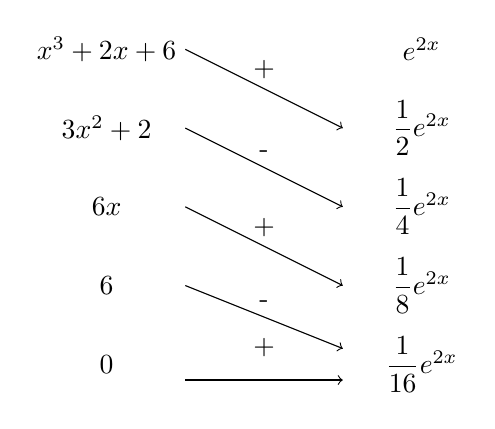
\begin{tikzpicture}
        \draw 
            (-2,3) node{$x^3+2x+6$}
            (-2,2) node{$3x^2+2$}
            (-2,1) node{$6x$}
            (-2,0) node{6}
            (-2,-1) node{0}
            (2,3) node{$e^{2x}$}
            (2,2) node{$\dfrac{1}{2}e^{2x}$}
            (2,1) node{$\dfrac{1}{4}e^{2x}$}
            (2,0) node{$\dfrac{1}{8}e^{2x}$}
            (2,-1) node{$\dfrac{1}{16}e^{2x}$};
        \path [->]
            (-1,3) edge node[midway, above]{+} (1,2)
            (-1,2) edge node[midway, above]{-} (1,1)
            (-1,1) edge node[midway, above]{+} (1,0)
            (-1,0) edge node[midway, above]{-} (1,-0.8)
            (-1,-1.2) edge node[midway, above=5pt]{+} (1,-1.2);
    \end{tikzpicture}
\end{center}

利用上述方法,可得
\begin{equation}
    \begin{aligned}
        \mbox{原式}&=(x^3+2x+6)\left(\dfrac{1}{2}e^{2x}\right)-(3x^2+2)\left(\dfrac{1}{4}e^{2x}\right)+6x\left(\dfrac{1}{8}e^{2x}\right)-6\left(\dfrac{1}{16}e^{2x}\right)+\int0\cdot\left(\dfrac{1}{16}e^{2x}\right)\deriv x \\
        &=\left(\dfrac{1}{2}x^3-\dfrac{3}{4}x^2+\dfrac{7}{4}x+\dfrac{17}{8}\right)e^{2x}+C
    \end{aligned}
    \nonumber
\end{equation}

\section{有理函数的积分}
\textbf{1.有理函数的积分} \quad 形如$\displaystyle\int\dfrac{P_n(x)}{Q_m(x)}\deriv x,(n<m)$的积分称为有理函数的积分,其中$P_n(x),Q_m(x)$分别是$x$的$n$次多项式和$m$次多项式.

若要计算,应先将$Q_m(x)$因式分解,再把$\dfrac{P_n(x)}{Q_m(x)}$拆成若干项最简有理分式之和.

分解的基本原则

(1)$Q_m(x)$的一次单因式$ax+b$产生一项$\dfrac{A}{ax+b}$.
\vspace{2mm}

(2)$Q_m(x)$的$k$重一次因式$(ax+b)^k$产生$k$项$\dfrac{A_1}{ax+b}+\dfrac{A_2}{(ax+b)^2}+\cdots+\dfrac{A_k}{(ax+b)^k}$.
\vspace{2mm}

(3)$Q_m(x)$的二次单因式$px^2+qx+r$产生一项$\dfrac{Ax+B}{px^2+qx+r}$.
\vspace{2mm}

(4)$Q_m(x)$的$k$重二次因式$(px^2+qx+r)^k$产生$k$项
\begin{equation}
    \dfrac{A_1 x+B_1}{px^2+qx+r}+\dfrac{A_2 x+B_2}{(px^2+qx+r)^2}+\cdots+\dfrac{A_k x+B_k}{(px^2+qx+r)^k}
    \nonumber
\end{equation}

\textbf{2.三角函数有理式的积分} \quad 一般有以下三种方法:
\vspace{2mm}

(1)半角代换 \quad 对于$\displaystyle\int R(\sin x,\cos x)\deriv x$型,令$\tan\dfrac{x}{2}=t$化为有理函数的积分

(2)三角恒等变换

1)利用倍角公式降低三角函数的幂次.
\vspace{2mm}

2)对于$\displaystyle\int\sin mx\cdot\sin nx\deriv x,\int\sin mx\cdot\cos nx\deriv x,\int\cos mx\cdot \cos nx\deriv x \quad (m\neq n)$可利用积化和差来计算.
\vspace{2mm}

3)对于$\displaystyle\int \sin^m x\cdot \cos^n x\deriv x$:(i)当$m,n$中有一个奇数,可拆开用凑微分法计算;(ii)当$m,n$都是偶数,可利用倍角公式逐步求出积分;
\vspace{2mm}

4)对于$\displaystyle\int\sin^n x\deriv x,\int\cos^n x\deriv x$,可利用分部积分法导出的递推公式计算,也可按3)处理.
\vspace{2mm}

\textbf{3.简单无理函数的积分} \quad 关键是找出适当的变量代换去掉根号,化为有理函数的积分.
    \setcounter{chapter}{4}

\chapter{定积分}

\begin{introduction}
    \item 定积分的定义 \ref{def:definite_integral}
    \item 微积分基本公式
    \item 定积分的换元法和分部积分法
    \item 广义积分
\end{introduction}

\section{定积分的概念与性质}
\begin{definition}[定积分的定义] \label{def:definite_integral}
    设$f(x)$是定义在区间$[a,b]$上的有界函数,任取分点$a=x_0<x_1<x_2<\cdots<x_n=b$,将$[a,b]$分为$n$个子区间$[x_{i-1},x_i]$,记$\Delta x_i=x_i-x_{i-1},(i=1,2,\cdots,n)$,又在每个子区间上任取一点$\xi_i\in[x_{i-1},x_i],(i=1,2,\cdots,n)$,若不论对区间$[a,b]$如何分法,也不论$\xi_i$在$[x_{i-1},x_i]$中如何取法,只要当$\displaystyle\lambda=\max_{1\leq i\leq n}\Delta x_i$趋于零时,和式$\displaystyle\sum_{i=1}^n f(\xi_i)\Delta x_i$的极限存在,则称此极限值为$f(x)$在$[a,b]$上的定积分,记为
    \begin{equation}
        \int_a^b f(x)\deriv x = \lim_{\lambda\rightarrow0}\sum_{i=1}^n f(\xi_i)\Delta x_i
        \nonumber
    \end{equation}

    此时也称$f(x)$在$[a,b]$上可积.

    特别地,把区间$[a,b]$分为$n$等份,$\xi_i$取为每个小区间的右端点,则有
    \begin{equation}
        \begin{aligned}
            &\lim_{n\rightarrow\infty}\dfrac{b-a}{n}\sum_{i=1}^n f\left(a+\dfrac{b-a}{n}i\right)=\int_a^b f(x)\deriv x \\
            &\lim_{n\rightarrow\infty}\dfrac{1}{n}\sum_{i=1}^n f\left(\dfrac{i}{n}\right)=\int_0^1 f(x)\deriv x  \quad (\mbox{此时}a=0,b=1)
        \end{aligned}
        \nonumber
    \end{equation}

    使用以上两个公式可计算某些和式的极限
\end{definition}

\begin{property} \label{property:definite_integral}
    \begin{enumerate}
        \item 定积分的结果与积分变量无关,即$\displaystyle\int_a^b f(x)\deriv x=\int_a^b f(t)\deriv t$
        \item $\displaystyle\int_a^a f(x)\deriv x\equiv0$
        \item $\displaystyle\int_b^a f(x)\deriv x=-\int_a^b f(x)\deriv x$
        \item 若$f(x)$在$[a,b]$上可积,$k$为任一常数,则$\displaystyle\int_a^b kf(x)\deriv x=k\int_a^b f(x)\deriv x$
        \item 若$f(x),g(x)$在$[a,b]$上都可积,则
            \begin{equation}
                \int_a^b [f(x)\pm g(x)]\deriv x=\int_a^bf(x)\deriv x\pm\int_a^b g(x)\deriv x
                \nonumber
            \end{equation}
        \item 设函数$f(x)$在$[a,c],[c,b],[a,b]$上都可积,则
            \begin{equation}
                \int_a^b f(x)\deriv x=\int_a^c f(x)\deriv x+\int_c^b f(x)\deriv x
                \nonumber
            \end{equation}

        当$c$点在$[a,b]$外时,结论仍成立
        \item 设$f(x),g(x)$在$[a,b]$上可积,且满足不等式$f(x)\leq g(x),x\in[a,b]$,则
            \begin{equation}
                \int_a^b f(x)\deriv x\leq \int_a^b g(x)\deriv x
                \nonumber
            \end{equation}
        \item 估值定理 \quad 设$f(x)$在$[a,b]$上的最大值、最小值分别为$M$和$m$,则有
            \begin{equation}
                m(b-a)\leq \int_a^b f(x)\deriv x\leq M(b-a)
                \nonumber
            \end{equation}
        \item 积分中值定理 \quad 设$f(x)$在$[a,b]$上连续,则在$[a,b]$上至少存在一点$\xi$,使得
            \begin{equation}
                \int_a^b f(x)\deriv x=f(\xi)(b-a)
                \nonumber
            \end{equation}

            称$\displaystyle\dfrac{1}{b-a}\int_a^b f(x)\deriv x$为函数$f(x)$在$[a,b]$上的积分平均值
    \end{enumerate}
\end{property}
\vspace{2mm}

\textbf{积分不等式} \quad 设$f(x),g(x)$在区间$[a,b]$上可积,则有下列不等式
\vspace{2mm}

(1)$\displaystyle\left|\int_a^b f(x)\deriv x\right|\leq \int_a^b\left|f(x)\right|\deriv x$
\vspace{2mm}

(2)许瓦尔兹不等式
\begin{equation}
    \left[\int_a^b f(x)g(x)\deriv x\right]^2\leq \int_a^b[f(x)]^2\deriv x\cdot\int_a^b[g(x)]^2\deriv x
    \nonumber
\end{equation}

\textbf{一元函数的(常义)可积性}

(1)定积分存在的充分条件

(i)若$f(x)$在$[a,b]$上连续,则$\displaystyle\int_a^b f(x)\deriv x$存在.

(ii)若$f(x)$在$[a,b]$上单调,则$\displaystyle\int_a^b f(x)\deriv x$存在.

(iii)若$f(x)$在$[a,b]$上有界,且只有有限个间断点,则$\displaystyle\int_a^b f(x)\deriv x$存在.

(1)定积分存在的必要条件

可积函数必有界,即若定积分$\displaystyle\int_a^b f(x)\deriv x$存在,则$f(x)$在$[a,b]$上必有界.

\section{微积分基本公式}
\textbf{1.变上限定积分}

(1)若$f(x)$在$[a,b]$上连续,则$\Phi(x)=\displaystyle\int_a^x f(t)\deriv t$在$[a,b]$上可导,且有
\begin{equation}
    \Phi'(x)=\dfrac{\deriv}{\deriv x}\int_a^x f(t)\deriv t=f(x)
    \nonumber
\end{equation}

(2)若$f(x)$在$[a,b]$上连续,$g(x)$是可微的,则
\begin{equation}
    \dfrac{\deriv}{\deriv x}\left(\int_a^{g(x)} f(t)\deriv t\right)=f[g(x)]g'(x)
    \nonumber
\end{equation}

(3)若上、下限都是$x$的可微函数,则
\begin{equation}
    \dfrac{\deriv}{\deriv x}\left(\int_{a(x)}^{b(x)} f(t)\deriv t\right)=f[b(x)]b'(x)-f[a(x)]a'(x)
    \nonumber
\end{equation}

实际上,这是一个求复合函数的导数问题.

\begin{property} \label{property:integral_with_variable_limit}

    (1)函数$f(x)$在$[a,b]$上可积,则函数$F(x)=\displaystyle\int_a^x f(t)\deriv t$在$[a,b]$上连续.

    (2)函数$f(x)$在$[a,b]$上连续,则函数$F(x)=\displaystyle\int_a^x f(t)\deriv t$在$[a,b]$上可导.
\end{property}

\textbf{2.定积分和不定积分的关系}

(1)原函数存在定理 \quad 若函数$f(x)$在$[a,b]$上连续,则函数$\Phi(x)=\displaystyle\int_a^x f(t)\deriv t$是$f(x)$在$[a,b]$区间上的一个原函数.

(2)牛顿-莱布尼茨公式 \quad 若$F(x)$是$f(x)$在区间$[a,b]$上的一个原函数,而且$f(x)$在$[a,b]$上连续,则
\begin{equation}
    \int_a^b f(x)\deriv x=F(b)-F(a)
    \nonumber
\end{equation}

这个公式也称为微积分基本公式,它指出了定积分与不定积分的内在联系.

\section{定积分的换元法和分部积分法}
\textbf{1.换元积分法} \quad 若函数$f(x)$在区间$[a,b]$上连续;函数$x=\varphi(t)$在区间$[\alpha,\beta]$上单调且具有连续导数,当$\alpha\leq t\leq\beta$时,$a\leq\varphi(t)\leq b$,且$\varphi(\alpha)=a,\varphi(\beta)=b$,则有定积分的换元公式
\begin{equation}
    \int_a^b f(x)\deriv x=\int_{\alpha}^{\beta} f[\varphi(t)]\varphi'(t)\deriv t
    \nonumber
\end{equation}

\textbf{2.分部积分法} \quad 设函数$u(x),v(x)$在区间$[a,b]$上具有连续导数$u'(x),v'(x)$,则有定积分的分部积分公式
\begin{equation}
    \int_a^b u(x)v'(x)\deriv x=[u(x)v(x)] \bigg|_a^b - \int_a^bv(x)u' (x)\deriv x
    \nonumber
\end{equation}

\textbf{3.常用公式} \quad 设$f(x)$为连续函数
\vspace{2mm}

(1)$\displaystyle\int_{-a}^a f(x)\deriv x=\int_0^a[f(x)+f(-x)]\deriv x$

(2)$\displaystyle\int_{-a}^a f(x) \deriv x=\left\{
\begin{aligned}
&2\int_0^a f(x)\deriv x,  &f(x)\mbox{是偶函数} \\
&0, &f(x)\mbox{是奇函数}
\end{aligned}
\right.$

(3)$\displaystyle\int_0^{\frac{\pi}{2}} f(\sin x)\deriv x=\int_0^{\frac{\pi}{2}} f(\cos x)\deriv x$
\vspace{2mm}

(4)$\displaystyle\int_0^\pi xf(\sin x)\deriv x=\dfrac{\pi}{2}\int_0^\pi f(\sin x)\deriv x$

(5)$f(x+L)=f(x),(L>0)$,则$\displaystyle\int_0^L f(x)\deriv x=\int_{-\frac{L}{2}}^{\frac{L}{2}}f(x)\deriv x=\int_a^{a+L} f(x)\deriv x$

(6)$\displaystyle\int_0^{\frac{\pi}{2}}(\sin x)^n\deriv x=\int_0^{\frac{\pi}{2}}(\cos x)^n\deriv x=\left\{ 
\begin{aligned}
    & \dfrac{(n-1)!!}{n!!}\cdot \dfrac{\pi}{2}, &\mbox{当}n\mbox{为偶数时} \\
    & \dfrac{(n-1)!!}{n!!}, &\mbox{当}n\mbox{为奇数时} \\
\end{aligned}\right.$

(7)$\displaystyle\int_a^b f(x)\deriv x=\int_a^b f(a+b-x)\deriv x$ \quad (区间再现公式)

\section{广义积分}
\textbf{1.无穷区间上的广义积分} \quad 设函数$f(x)$在区间$[a,+\infty)$上有定义,在$[a,b](b<+\infty)$上可积,若极限$\displaystyle\lim_{b\rightarrow+\infty}\int_a^b f(x)\deriv x$存在,则定义
\begin{equation}
    \int_a^{+\infty} f(x)\deriv x=\lim_{b\rightarrow +\infty}\int_a^b f(x)\deriv x
    \nonumber
\end{equation}

并称$\displaystyle\int_a^{+\infty} f(x)\deriv x$为$f(x)$在$[a,+\infty)$上的广义积分,这时也称广义积分$\displaystyle\int_a^{+\infty} f(x)\deriv x$存在或收敛;若上述极限不存在,则称广义积分$\displaystyle\int_a^{+\infty} f(x)\deriv x$不存在或发散.

类似地,定义
\begin{equation}
    \begin{aligned}
        &\int_{-\infty}^b f(x)\deriv x=\lim_{a\rightarrow-\infty}\int_a^b f(x)\deriv x \\
        &\int_{-\infty}^{+\infty}f(x)\deriv x=\int_{-\infty}^c f(x)\deriv x+\int_c^{+\infty} f(x)\deriv x=\lim_{a\rightarrow-\infty}\int_a^cf(x)\deriv x+\lim_{b\rightarrow+\infty}\int_c^b f(x)\deriv x
    \end{aligned}
    \nonumber
\end{equation}

\textbf{2.无界函数的广义积分(瑕积分)} \quad 设函数$f(x)$在区间$[a,b)$上连续,而且$\displaystyle\lim_{x\rightarrow b^-}f(x)=\infty$,若极限\\$\displaystyle\lim_{\varepsilon\rightarrow0^+}\int_a^{b-\varepsilon} f(x)\deriv x$存在,则定义
\begin{equation}
    \int_a^b f(x)\deriv x=\lim_{\varepsilon\rightarrow0^+}\int_a^{b-\varepsilon} f(x)\deriv x
    \nonumber
\end{equation}

并称$\displaystyle\int_a^b f(x)\deriv x$为$f(x)$在$[a,b)$上的广义积分,这时也称广义积分$\displaystyle\int_a^b f(x)\deriv x$存在或收敛;若上述极限不存在,则称广义积分$\displaystyle\int_a^{+\infty} f(x)\deriv x$不存在或发散.

类似地,若$f(x)$在$(a,b]$上连续,$\displaystyle\lim_{x\rightarrow a^+} f(x)=\infty$,则定义
\begin{equation}
    \int_a^b f(x)\deriv x=\lim_{\varepsilon\rightarrow 0^+}\int_{a+\varepsilon}^b f(x)\deriv x
    \nonumber
\end{equation}

若$f(x)$在$(a,b)$上连续,$\displaystyle\lim_{x\rightarrow a^+} f(x)=\infty,\lim_{x\rightarrow b^-} f(x)=\infty$,则定义
\begin{equation}
    \int_a^b f(x)\deriv x=\lim_{\varepsilon_1\rightarrow 0^+}\int_{a+\varepsilon_1}^c f(x)\deriv x+\lim_{\varepsilon_2\rightarrow0^+}\int_c^{b-\varepsilon_2} f(x)\deriv x
    \nonumber
\end{equation}

\textbf{3.反常积分敛散性判别的两个重要结论}
\vspace{2mm}

(1)无穷区间的反常积分$\displaystyle\int_1^{+\infty}\dfrac{\deriv x}{x^p}$:在$p>1$时收敛,在$p\leq1$时发散.
\vspace{2mm}

(2)无界函数的反常积分$\displaystyle\int_0^1\dfrac{\deriv x}{x^p},(p>0,\mbox{奇点}\ x=0)$:在$0<p<1$时收敛,在$p\geq1$时发散.
    \setcounter{chapter}{5}

\chapter{定积分的应用}

\begin{introduction}
    \item 平面图形的面积
    \item 旋转体的体积
    \item 旋转曲面的面积
    \item 弧长公式
\end{introduction}

\section{定积分在几何上的应用}
\textbf{1.平面图形的面积}

(1)直角坐标情形:

由连续曲线$y=f_1(x),y=f_2(x),(f_1(x)\leq f_2(x))$与直线$x=a,x=b$围成的图形面积$(a\leq b)$
\begin{equation}
    A=\int_a^b [f_2(x)-f_1(x)]\deriv x
    \nonumber
\end{equation}

由连续曲线$x=g_1(y),x=g_2(y),(g_1(y)\leq g_2(y))$与直线$y=c,y=d$围成的图形面积$(a\leq b)$
\begin{equation}
    A=\int_c^d [g_2(y)-g_1(y)]\deriv y
    \nonumber
\end{equation}

(2)极坐标情形:由连续曲线$r=r_1(\theta)$与$r=r_2(\theta)$与两射线$\theta=\alpha,\theta=\beta,(0<\beta-\alpha\leq 2\pi)$围成的曲边扇形的面积
\begin{equation}
    A=\dfrac{1}{2}\int_\alpha^\beta \left|r_1^2(\theta)-r_2^2(\theta)\right|\deriv \theta
    \nonumber
\end{equation}

\textbf{2.旋转体的体积}

(1)曲线$y=y(x)$与$x=a,x=b,(a<b)$及$x$轴围成的曲边梯形绕$x$轴旋转一周所得到的旋转体的体积
\begin{equation}
    V=\pi\int_a^b y^2\deriv x=\pi \int_a^b f^2(x)\deriv x
    \nonumber
\end{equation}

(2)曲线$x=x(y)$与$y=c,y=d,(c<d)$及$y$轴围成的曲边梯形绕$y$轴旋转一周所得到的旋转体的体积
\begin{equation}
    V=\pi\int_c^d x^2\deriv y=\pi \int_c^d g^2(y)\deriv y
    \nonumber
\end{equation}

(3)曲线$y=y_1(x)\geq0$与$y=y_2(x)\geq0$及$x=a,x=b,(a<b)$所围成的平面图形绕$x$轴旋转一周所得到的旋转体的体积
\begin{equation}
    V=\pi\int_a^b \left| y_1^2(x)-y_2^2(x) \right| \deriv x
    \nonumber
\end{equation}

(4)曲线$y=y(x)$与$x=a,x=b,(0\leq a<b)$及$x$轴围成的曲边梯形绕$y$轴旋转一周所得到的旋转体的体积
\begin{equation}
    V_y=2\pi\int_a^b x\left|y(x)\right| \deriv x
    \nonumber
\end{equation}

(5)曲线$y=y_1(x)$与$y=y_2(x)$及$x=a,x=b(0\leq a\leq b)$所围成的图形绕$y$轴旋转一周所成的旋转体的体积
\begin{equation}
    V=2\pi\int_a^b x\left|y_1(x)-y_2(x)\right| \deriv x
    \nonumber
\end{equation}

\textbf{3.旋转曲面的面积}

(1)光滑曲线$y=f(x),(a\leq x\leq b)$绕$x$轴旋转而成的旋转曲面面积
\begin{equation}
    S=2\pi \int_a^b \left|y\right|\sqrt{1+y'^2} \deriv x
    \nonumber
\end{equation}

(2)光滑曲线$\left\{\begin{aligned}
    x=x(t) \\
    y=y(t)
\end{aligned}\right.,(\alpha\leq t\leq \beta)$绕$x$轴旋转而成的旋转曲面面积
\begin{equation}
    S=2\pi \int_\alpha^\beta \left|y(t)\right|\sqrt{[x'(t)]^2+[y'(t)]^2}\deriv t
    \nonumber
\end{equation}

\textbf{4.曲线的弧长公式}

(1)光滑曲线$y=f(x),(a\leq x\leq b)$的弧长为
\begin{equation}
    l=\int_a^b\sqrt{1+[y'(x)]^2}\deriv x=\int_a^b\sqrt{1+[f'(x)]^2}\deriv x
    \nonumber
\end{equation}

(2)光滑曲线$\left\{\begin{aligned}
    x=x(t) \\
    y=y(t)
\end{aligned}\right.,(\alpha\leq t\leq \beta)$的弧长为
\begin{equation}
    l=\int_\alpha^\beta\sqrt{[x'(t)]^2+[y'(t)]^2}\deriv t
    \nonumber
\end{equation}

(3)光滑曲线$r=r(\theta),\varphi_0\leq\theta\leq\varphi_1$的弧长
\begin{equation}
    l=\int_{\varphi_0}^{\varphi_1}\sqrt{r^2+r'^2}\deriv \theta
    \nonumber
\end{equation}

\textbf{5.用定积分表达和计算函数的平均值}

设$x\in[a,b]$,函数$y(x)$在$[a,b]$上的平均值为$\bar{y}=\dfrac{1}{b-a}\displaystyle\int_a^b y(x)\deriv x$
    \setcounter{chapter}{6}

\chapter{向量代数与空间解析几何}

\begin{introduction}
    \item 向量的运算
    \item 空间的平面和直线
    \item 空间曲面与空间曲线
\end{introduction}

\section{向量及其运算}
\textbf{向量的数量积(点乘积或内积)}

向量$\bm{a}=\{a_1,a_2,a_3\}$与$\bm{b}=\{b_1,b_2,b_3\}$的数量积是一个数$\left|\bm{a}\right|\cdot\left|\bm{b}\right|\cos\overset{\wedge}{(\bm{a},\bm{b})}$,(且$0\leq \overset{\wedge}{(\bm{a},\bm{b})}\leq \pi$,记作$\bm{a}\cdot\bm{b}$。若向量$\bm{a}$或$\bm{b}$为零向量时,则定义$\bm{a}\cdot\bm{b}=0$,数量积$\bm{a}\cdot\bm{b}$的坐标表示式为
\begin{equation}
    \bm{a}\cdot\bm{b}=a_1 b_1+a_2 b_2+a_3 b_3
    \nonumber
\end{equation}

两个向量$\bm{a},\bm{b}$垂直(或称正交),记作$\bm{a}\perp\bm{b}$,特别地,规定零向量与任意向量垂直。

\begin{property} \label{property:dot_product}
    \begin{enumerate}
        \item $\bm{a}\cdot\bm{b} = \bm{b}\cdot\bm{a}$
        \item $(\lambda \bm{a})\cdot\bm{b} = \lambda(\bm{a}\cdot\bm{b})$
        \item $(\bm{a}+\bm{b})\cdot\bm{c}=\bm{a}\cdot\bm{c}+\bm{b}\cdot\bm{c}$
        \item $\bm{a}\perp\bm{b}$的充分必要条件是$\bm{a}\cdot\bm{b}=0$
    \end{enumerate}
\end{property}
\vspace{2mm}

\textbf{向量的向量积(叉乘积或外积)}

两个向量$\bm{a}$和$\bm{b}$的向量积是一个向量$\bm{c}$,记为$\bm{a}\times\bm{b}$,即$\bm{c}=\bm{a}\times\bm{b}$;$\bm{c}$的模等于$|\bm{a}||\bm{b}|\sin\overset{\wedge}{(\bm{a},\bm{b})}$,$\bm{c}$的方向垂直于$\bm{a}$与$\bm{b}$所决定的平面,且$\bm{a},\bm{b},\bm{c}$顺次构成右手系,若向量$\bm{a}$或$\bm{b}$为零向量时,则定义$\bm{a}\times\bm{b}=0$,向量积$\bm{a}\times\bm{b}$坐标表示式为:
\begin{equation} 
    \bm{a}\times\bm{b}=
    \begin{vmatrix}
        \bm{i} & \bm{j} & \bm{k} \\
        a_1 & a_2 & a_3 \\
        b_1 & b_2 & b_3
    \end{vmatrix}
    = \left\{
        \begin{vmatrix}
            a_2 & a_3 \\
            b_2 & b_3
        \end{vmatrix},
        -\begin{vmatrix}
            a_1 & a_3 \\
            b_1 & b_3
        \end{vmatrix},
        \begin{vmatrix}
            a_1 & a_2 \\
            b_1 & b_2
        \end{vmatrix}
    \right\}
    \nonumber
\end{equation}

\begin{property} \label{property:cross_product}
    \begin{enumerate}
        \item $\bm{a}\times\bm{b} = -\bm{b}\times\bm{a}$
        \item $(\lambda \bm{a})\times\bm{b} = \lambda(\bm{a}\times\bm{b})$
        \item $(\bm{a}+\bm{b})\times\bm{c}=\bm{a}\times\bm{c}+\bm{b}\times\bm{c}$
        \item $\bm{a}\pll\bm{b}$的充分必要条件是$\bm{a}\times\bm{b}=0$
    \end{enumerate}
\end{property}
\vspace{2mm}

\textbf{向量的混合积}

设$\bm{a}=\{a_1,a_2,a_3\},\bm{b}=\{b_1,b_2,b_3\},\bm{c}=\{c_1,c_2,c_3\}$,则称乘积$(\bm{a}\times\bm{b})\cdot\bm{c}$为向量$\bm{a},\bm{b},\bm{c}$的混合积,记为$[\bm{a},\bm{b},\bm{c}]$。

混合积是一数量,其几何意义为:混合积的绝对值等于以$\bm{a},\bm{b},\bm{c}$为相邻三条棱的平行六面体的体积。因此,向量$\bm{a},\bm{b},\bm{c}$共面的充分必要条件是\quad $(\bm{a}\times\bm{b})\cdot\bm{c}=0$

混合积$(\bm{a}\times\bm{b})\cdot\bm{c}$的坐标表达式为
\begin{equation}
    (\bm{a}\times\bm{b})\cdot\bm{c}=
    \begin{vmatrix}
        a_1 & a_2 & a_3 \\
        b_1 & b_2 & b_3 \\
        c_1 & c_2 & c_3
    \end{vmatrix}
    \nonumber
\end{equation}

且
\begin{equation}
    (\bm{a}\times\bm{b})\cdot\bm{c}=(\bm{b}\times\bm{c})\cdot\bm{a}=(\bm{c}\times\bm{a})\cdot\bm{b}
    \nonumber
\end{equation}

\begin{note}
本节的内容可以用行列式的性质去理解记忆
\end{note}

\section{空间的平面和直线}
\textbf{1.平面及其方程}

法向量 \quad 与平面垂直的任意非零向量,称为该平面的法向量.

(1)点法式方程 \quad 设平面过点$M_0(x_0,y_0,z_0)$,其法向量为$\bm{n}=\{A,B,C\}$,则此平面方程为
\begin{equation}
    A(x-x_0)+B(y-y_0)+C(z-z_0)=0
    \nonumber
\end{equation}

(2)截距式方程 \quad 设$a,b,c$分别为平面在$x,y,z$轴上的截距,则此平面方程为
\begin{equation}
    \frac{x}{a}+\frac{y}{b}+\frac{z}{c}=1
    \nonumber
\end{equation}

(3)三点式方程 \quad 设平面过不共线的三点$A(x_1,y_1,z_1),B(x_2,y_2,z_2),C(x_3,y_3,z_3)$,则此平面方程为
\begin{equation}
    \begin{vmatrix}
        x-x_1 & y-y_1 & z-z_1 \\
        x_2-x_1 & y_2-y_1 & z_2-z_1 \\
        x_3-x_1 & y_3-y_1 & z_3-z_1
    \end{vmatrix}=0
    \nonumber
\end{equation}

(4)一般式方程 \quad 平面的一般式方程是三元一次方程
\begin{equation}
    Ax+By+Cz+D=0
    \nonumber
\end{equation}
其中$A,B,C$不同时为零.

\textbf{2.空间直线及其方程}

方向向量 \quad 与直线平行的非零向量,称为该直线的方向向量.

(1)对称式方程(又称点向式或标准式方程)

过点$M_0(x_0,y_0,z_0)$,方向向量为$\bm{s}=\{l,m,n\}$的直线的标准式方程为
\begin{equation}
    \frac{x-x_0}{l}=\frac{y-y_0}{m}=\frac{z-z_0}{n}
    \nonumber
\end{equation}

(2)参数方程 \quad 由标准式方程
\begin{equation}
    \frac{x-x_0}{l}=\frac{y-y_0}{m}=\frac{z-z_0}{n}=t
    \nonumber
\end{equation}
易得直线的参数方程
\begin{equation}
    \begin{cases}
    x=x_0+lt \\
    y=y_0+mt \\
    z=z_0+nt
    \end{cases}
    \quad (t\mbox{为参数})
    \nonumber
\end{equation}

(3)两点式方程 \quad 过点$M_1(x_1,y_1,z_1),M_2(x_2,y_2,z_2)$的直线方程为
\begin{equation}
    \frac{x-x_1}{x_2-x_1}=\frac{y-y_1}{y_2-y_1}=\frac{z-z_1}{z_2-z_1}
    \nonumber
\end{equation}

(4)一般式方程 \quad 直线的一般式方程是三元一次方程
\begin{equation}
    \begin{cases}
    A_1x+B_1y+C_1z+D_1=0 \\
    A_2x+B_2y+C_2z+D_2=0
    \end{cases}
    \nonumber
\end{equation}
其中每一个三元一次方程都表示一个平面.

\textbf{3.直线、平面之间的相对位置关系}

设平面 \quad $\pi_1:A_1x+B_1y+C_1z+D_1=0 \quad \pi_2:A_2x+B_2y+C_2z+D_2=0$,它们的法向量分别为$\bm{n}_1=\{A_1,B_1,C_1\},\bm{n}_2=\{A_2,B_2,C_2\}$

直线 \quad $L_1:\dfrac{x-x_1}{l_1}=\dfrac{y-y_1}{m_1}=\dfrac{z-z_1}{n_1} \quad L_2:\dfrac{x-x_2}{l_2}=\dfrac{y-y_2}{m_2}=\dfrac{z-z_2}{n_2}$,它们的方向向量分别为$\bm{s}_1=\{l_1,m_1,n_1\},\bm{s}_2=\{l_2,m_2,n_2\}$

(1)夹角

平面$\pi_1$与$\pi_2$的夹角$\theta$定义为法向量$\bm{n}_1,\bm{n}_2$的夹角,即
\begin{equation}
    \cos\theta=\dfrac{\bm{n}_1\cdot\bm{n}_2}{|\bm{n}_1|\cdot|\bm{n}_2|}=\dfrac{|A_1A_2+B_1B_2+C_1C_2|}{\sqrt{A_1^2+B_1^2+C_1^2}\cdot\sqrt{A_2^2+B_2^2+C_2^2}}
    \nonumber
\end{equation}

直线$L_1$与$L_2$的夹角$\theta$定义为方向向量$\bm{s}_1,\bm{s}_2$的夹角,即
\begin{equation}
    \cos\theta=\dfrac{\bm{s}_1\cdot\bm{s}_2}{|\bm{s}_1|\cdot|\bm{s}_2|}=\dfrac{|l_1l_2+m_1m_2+n_1n_2|}{\sqrt{l_1^2+m_1^2+n_1^2}\cdot\sqrt{l_2^2+m_2^2+n_2^2}}
    \nonumber
\end{equation}

直线$L_1$与平面$\pi_1$的夹角$\theta$定义为直线$L_1$和它在平面$\pi_1$上的投影所成的两邻角中的锐角,即
\begin{equation}
    \sin\theta=\dfrac{|\bm{s}_1\cdot\bm{n}_1|}{|\bm{s}_1|\cdot|\bm{n}_1|}=\dfrac{|A_1l_1+B_1m_1+C_1n_1|}{\sqrt{A_1^2+B_1^2+C_1^2}\cdot\sqrt{l_1^2+m_1^2+n_1^2}}
    \nonumber
\end{equation}

(2)平行的条件

平面$\pi_1$与$\pi_2$平行的充分必要条件是$\dfrac{A_1}{A_2}=\dfrac{B_1}{B_2}=\dfrac{C_1}{C_2}$

直线$L_1$与$L_2$平行的充分必要条件是$\dfrac{l_1}{l_2}=\dfrac{m_1}{m_2}=\dfrac{n_1}{n_2}$

直线$L_1$与平面$\pi_1$平行的充分必要条件是$l_1A_1+m_1B_1+n_1C_1=0$

(3)垂直的条件

平面$\pi_1$与$\pi_2$垂直的充分必要条件是$A_1A_2+B_1B_2+C_1C_2=0$

直线$L_1$与$L_2$垂直的充分必要条件是$l_1l_2+m_1m_2+n_1n_2=0$

直线$L_1$垂直于平面$\pi_1$的充分必要条件是$\dfrac{l_1}{A_1}=\dfrac{m_1}{B_1}=\dfrac{n_1}{C_1}$

\textbf{4.距离公式}

(1)点到平面的距离

点$M_0(x_0,y_0,z_0)$到平面$Ax+By+Cz+D=0$的距离为$d=\dfrac{|Ax_0+By_0+Cz_0+D|}{\sqrt{A^2+B^2+C^2}}$

(2)点到直线的距离

点$P_1(x_1,y_1,z_1)$到直线$\dfrac{x-x_0}{l}=\dfrac{y-y_0}{m}=\dfrac{z-z_0}{n}$的距离为$d=\dfrac{|\overrightarrow{M_0P_1}\times\bm{s}|}{|\bm{s}|}$,其中,
\begin{equation}
    M_0(x_0,y_0,z_0), \quad \bm{s}=\{l,m,n\}
    \nonumber
\end{equation}

(3)两直线共面的条件

设有两直线 \quad $L_1:\dfrac{x-x_1}{l_1}=\dfrac{y-y_1}{m_1}=\dfrac{z-z_1}{n_1}, \quad L_2:\dfrac{x-x_2}{l_2}=\dfrac{y-y_2}{m_2}=\dfrac{z-z_2}{n_2}$,共面的条件为$\overrightarrow{P_1P_2}\cdot(\bm{a}\times\bm{b})=0$,其中
\begin{equation}
    P_1(x_1,y_1,z_1), \quad P_2(x_2,y_2,z_2), \quad \bm{a}=\{l_1,m_1,n_1\}, \quad \bm{b}=\{l_2,m_2,n_2\}
\end{equation}

(4)两直线间的距离

两异面直线$L_1,L_2$的距离为$d=\dfrac{|\overrightarrow{P_1P_2}\cdot(\bm{a}\times\bm{b})|}{|\bm{a}\times\bm{b}|}$

\section{空间曲面与空间曲线}
\textbf{1.空间曲面方程}

(1)一般方程 $F(x,y,z)=0$

(2)显式方程 $z=f(x,y)$

(3)参数方程 $\left\{\begin{aligned}& x=x(u,v) \\ & y=y(u,v) \\ & z=z(u,v) \end{aligned}\right.$ \quad $(u,v)\in D$,其中$D$为$uv$平面上某一区域

\textbf{2.旋转曲面方程}

设$C:f(y,z)=0$为$yOz$平面上的曲线,则

(1)$C$绕$z$轴旋转所得的曲面为$f(\pm\sqrt{x^2+y^2},z)=0$

(2)$C$绕$y$轴旋转所得的曲面为$f(x,\pm\sqrt{y^2+z^2})=0$

旋转曲面主要由母线和旋转轴确定.

求旋转曲面方程时,平面曲线绕某坐标轴旋转,则该坐标轴对应的变量不变,而曲线方程中另一变量改写成该变量与第三变量平方和的正负平方根,例如:$L\left\{\begin{aligned}& f(x,y)=0 \\ & z=0 \end{aligned}\right.$.曲线$L$绕$x$轴旋转所形成的旋转曲面的方程为$f(x,\pm\sqrt{y^2+z^2})=0$

\textbf{3.柱面方程}

(1)母线平行于$z$轴的柱面方程为$F(x,y)=0$

(2)母线平行于$x$轴的柱面方程为$G(y,z)=0$

(3)母线平行于$y$轴的柱面方程为$H(x,z)=0$

当曲面方程中缺少一个变量时,则曲面为柱面,如$F(x,y)=0$,变量$z$未出现,该曲面表示由准线$\left\{\begin{aligned}& F(x,y)=0 \\ & z=0 \end{aligned}\right.$生成,母线平行于$z$轴的柱面.

柱面方程必须注意准线与母线两个要素

\newpage
\addcontentsline{toc}{section}{Problem Plus}
\section*{Problem Plus}
\begin{note}
    以下内容需要一定线性代数知识基础
\end{note}

你是否思考过一个问题,即为什么形如$Ax+By+Cz+D=0$这样的表达式表示出来的是一个平面?

我们举一个简单的例子,假设一个平面为$x+y+z=0$,那么可以将这个平面式拆分为矩阵形式:
\begin{equation}
    \begin{bmatrix}
        1 & 1 & 1
    \end{bmatrix}
    \begin{bmatrix}
        x \\ y \\ z
    \end{bmatrix}
    =0
    \nonumber
\end{equation}

而$x+y+z=0$这个平面实际上是$\begin{bmatrix} 1 & 1 & 1 \end{bmatrix}$的零空间(Nullspace),即我们现在将上式抽象为矩阵方程$\mathbf{A}\mathbf{x}=0$,所谓零空间,即可理解为这个系数矩阵所对应的基础解系张成(span)的空间。让我们接着往下:

因为$\begin{bmatrix} 1 & 1 & 1 \end{bmatrix}$已经是行最简阶梯形(Row Reduced Echelon Form),所以易得一个基础解系
\begin{equation*}
    \mathbf{x}=c_1\begin{bmatrix} -1 \\ 1 \\ 0 \end{bmatrix} + c_2\begin{bmatrix} -1 \\ 0 \\ 1 \end{bmatrix} \quad (c_1, c_2 \in \mathbb{R}).
\end{equation*}

细心的你可能会发现,在这个等式中,$\text{rank}(\mathbf{A})=1, \text{rank}(\mathbf{x})=2$,同时可以观察到一个规律,对于任何矩阵等式$\mathbf{Ax}=0$,都有$\text{rank}(\mathbf{A})+\text{rank}(\mathbf{x})\leq \text{the number of A's columns}$,而这两个秩所对应的两个空间,正是$\mathbf{A}$的列空间(column space)和$\mathbf{x}$的零空间(nullspace)。而这个零空间的两个向量张出来的面即为平面$x+y+z=0$。

\begin{figure}[H]
    \centering
    \centerline{\includegraphics[width=12cm]{figure/nullspace_for_2d_plane.png}}
    \caption{矩阵的零空间张出的平面表示} \label{nullspace}
\end{figure}

基于这个思考方式,我们也可以理解平面束为何可以表示一条直线,这里就不过多赘述了,留给读者思考。
    \setcounter{chapter}{7}

\chapter{多元函数微分法及其应用}

\begin{introduction}
    \item 多元函数基本概念
    \item 偏导数与全微分
    \item 多元复合函数的求导法则
    \item 隐函数的求导法则
    \item 多元函数微分学的几何应用
    \item 方向导数与梯度
    \item 多元函数的极值及其求法
\end{introduction}

\section{多元函数的基本概念}
\textbf{1.二元函数的概念}

设有变量$x,y$和$z$,如果变量$x,y$在一定范围内取定一组值时,变量$z$按照一定的法则,总有唯一确定的数值与之对应,则称$z$是$x,y$的二元函数,记为
\begin{equation*}
    z=f(x,y)
\end{equation*}
并称$x,y$为自变量.

自变量$x,y$的取值范围,叫做函数的定义域.

在空间直角坐标系中,二元函数$z=f(x,y)$的图形通常是一张曲面,它的定义域是这张曲面在$xOy$平面上的投影.

类似地,可以定义三元以及三元以上的函数。二元及二元以上的函数,统称多元函数.

\textbf{2.二元函数的极限}

设二元函数$z=f(x,y)$定义在平面点集$E$上,$P_0(x_0,y_0)$是$E$的聚点,$A$为一常数。若对于任意给定的正数$\varepsilon$,总存在正数$\delta$,使得适合不等式$0<|P_0P|=\sqrt{(x-x_0)^2+(y-y_0)^2}<\delta$的一切点$P(x,y)$,都有
\begin{equation*}
    |f(x,y)-A|<\varepsilon
\end{equation*}
成立,则称$A$为函数$z=f(x,y)$当$x\rightarrow x_0, y\rightarrow y_0$时的极限,记为$\displaystyle \lim_{x\rightarrow x_0 \atop y\rightarrow y_0}f(x,y)=A$。这时也称当$x\rightarrow x_0, y\rightarrow y_0$时,函数$f(x,y)$收敛于$A$.

为了区别于一元函数极限,把上述二元函数的极限叫做二重极限.

所谓二重极限存在,是指点$P(x,y)$以任何方式无限趋于点$P_0(x_0,y_0)$时,函数$f(x,y)$都趋于同一数值$A$。因此,如果点$P(x,y)$以某一特殊方式,例如沿某一定直线或定曲线趋近于$P_0(x_0,y_0)$时,即使函数趋于某一确定值,也不能由此断定函数的极限存在。但是反过来,如果当$P(x,y)$以不同方式趋于$P_0(x_0,y_0)$时,函数趋于不同的值,那么就可以断定该函数的极限不存在.

\textbf{3.二元函数的连续性}

设函数$z=f(x,y)$的定义域为$D$,$P_0(x_0,y_0)$是$D$内的聚点,且$P_0\in D$,若
\begin{equation*}
    \lim_{x\rightarrow x_0 \atop y\rightarrow y_0}f(x,y)=f(x_0,y_0)
\end{equation*}
则称函数$z=f(x,y)$在点$P_0$处连续.

若函数在区域$D$内的每一点都连续,则称函数$z=f(x,y)$在区域$D$内连续.

多元初等函数在其定义域内是连续函数.

\textbf{4.有界闭区域上二元连续函数的性质}

\textbf{最大值和最小值定理} \quad 在有界闭区域上的二元连续函数,在该区域上至少取得它的最大值和最小值各一次.

\textbf{介值定理} \quad 在有界闭区域上的二元连续函数,如果取得两个不同的函数值,则函数在该区域上必取得介于这两个值之间的任何值.

特别地,若$\mu$是介于在有界闭区域上连续的函数$f(x,y)$的最小值$m$和最大值$M$之间的一个数,则在该区域中至少存在一点$P(\xi, \eta)$,使得$f(\xi, \eta)=\mu$.

\section{偏导数}
\textbf{1.偏导数定义}
\begin{align*}
    & \dfrac{\partial z}{\partial x}=\lim_{\Delta x\rightarrow 0}\dfrac{f(x+\Delta x,y)-f(x,y)}{\Delta x} \\
    & \dfrac{\partial z}{\partial y}=\lim_{\Delta y\rightarrow 0}\dfrac{f(x,y+\Delta y)-f(x,y)}{\Delta y}
\end{align*}

\textbf{2.高阶偏导数}

函数$z=f(x,y)$在区域$D$内的偏导数$f_x'(x,y),f_y'(x,y)$存在时,仍然是$x,y$的二元函数。若这两个函数的偏导数
\begin{align*}
    & \dfrac{\partial}{\partial x}\left(\dfrac{\partial z}{\partial x}\right)=\dfrac{\partial^2 z}{\partial x^2}=f_{xx}''(x,y) \\
    & \dfrac{\partial}{\partial y}\left(\dfrac{\partial z}{\partial x}\right)=\dfrac{\partial^2 z}{\partial x\partial y}=f_{xy}''(x,y) \\
    & \dfrac{\partial}{\partial x}\left(\dfrac{\partial z}{\partial y}\right)=\dfrac{\partial^2 z}{\partial y\partial x}=f_{yx}''(x,y) \\
    & \dfrac{\partial}{\partial y}\left(\dfrac{\partial z}{\partial y}\right)=\dfrac{\partial^2 z}{\partial y^2}=f_{yy}''(x,y)
\end{align*}
也存在,则称它们是函数$z=f(x,y)$的二阶偏导数.

二阶偏导数$\dfrac{\partial^2 z}{\partial x\partial y}$和$\dfrac{\partial^2 z}{\partial y\partial x}$称为函数$z=f(x,y)$的二阶混合偏导数。当这两个二阶混合偏导数在区域$D$内连续时,则在该区域$D$内有
\begin{equation*}
    \dfrac{\partial^2 z}{\partial x\partial y}=\dfrac{\partial^2 z}{\partial y\partial x}
\end{equation*}

\section{全微分}
\textbf{1.全微分的定义}

设$P_0(x_0,y_0)$为$f$定义域$D$内的一个内点,如果函数$z=f(x,y)$在点$P_0(x_0,y_0)$处的全增量$\Delta z$可表示为
\begin{equation*}
    \Delta z=f(x_0+\Delta x,y_0+\Delta y)-f(x_0,y_0)=A\cdot\Delta x+B\cdot\Delta y+o(\rho)
\end{equation*}
其中$A, B$是与$\Delta x, \Delta y$无关的常数。则称函数$z=f(x,y)$在点$P_0(x_0,y_0)$处可微,并称函数$z=f(x,y)$的全增量$\Delta z$的线性主部$A\cdot\Delta x+B\cdot\Delta y$为函数$z=f(x,y)$在点$P_0(x_0,y_0)$的全微分,记作
\begin{equation*}
    \deriv z=A\cdot\Delta x+B\cdot\Delta y=A\deriv x+B\deriv y \quad (\deriv x=\Delta x, \deriv y=\Delta y)
\end{equation*}
当函数$z=f(x,y)$在点$P_0(x_0,y_0)$处可微时有
\begin{equation*}
    \deriv z=f_x'(x_0,y_0)\deriv x+f_y'(x_0,y_0)\deriv y
\end{equation*}

\textbf{2.全微分的形式不变性}

设$z=f(u,v)$具有连续偏导数,$u=\varphi(x,y),v=\psi(x,y)$也具有连续偏导数,则复合函数$z=f[\varphi(x,y),\psi(x,y)]$在点$(x,y)$处的全微分为
\begin{equation*}
    \deriv z=\dfrac{\partial z}{\partial u}\deriv u+\dfrac{\partial z}{\partial v}\deriv v
\end{equation*}

\section{多元复合函数的求导法则}
\textbf{1.复合函数的偏导数}

设函数$u=\varphi(x,y),v=\psi(x,y)$在点$(x,y)$处存在偏导数,又函数$z=f(u,v)$在对应点$(u,v)$处具有连续的一阶偏导数,则复合函数$z=f[\varphi(x,y),\psi(x,y)]$在点$(x,y)$处对$x$及$y$的偏导数均存在,且有
\begin{equation*}
    \dfrac{\partial z}{\partial x}=\dfrac{\partial z}{\partial u}\cdot\dfrac{\partial u}{\partial x}+\dfrac{\partial z}{\partial v}\cdot\dfrac{\partial v}{\partial x}, \quad
    \dfrac{\partial z}{\partial y}=\dfrac{\partial z}{\partial u}\cdot\dfrac{\partial u}{\partial y}+\dfrac{\partial z}{\partial v}\cdot\dfrac{\partial v}{\partial y}
\end{equation*}

\textbf{2.全导数}
设函数$z=f(u,v)$,而$u=\varphi(x),v=\psi(x)$,则$z=f[\varphi(x),\psi(x)]$是$x$的一元函数,且
\begin{equation*}
    \dfrac{\deriv z}{\deriv x}=\dfrac{\partial z}{\partial u}\cdot\dfrac{\deriv u}{\deriv x}+\dfrac{\partial z}{\partial v}\cdot\dfrac{\deriv v}{\deriv x}
\end{equation*}
称$\dfrac{\deriv z}{\deriv x}$为$z$关于$x$的全导数。

\section{隐函数的求导法则}
\textbf{1.一元隐函数求导法则}

设函数$F(x,y)$在点$P(x_0,y_0)$的某个邻域内具有连续的偏导数$F_x'(x,y),F_y'(x,y)$,且$F(x_0,y_0)=0,F_y'(x_0,y_0)\neq 0$,则在$(x_0,y_0)$的某邻域内,方程$F(x,y)=0$恒能唯一确定一个具有连续导数的函数$y=f(x)$,它满足条件$y_0=f(x_0)$,并有
\begin{equation*}
    \dfrac{\deriv y}{\deriv x}=-\dfrac{F_x'(x,y)}{F_y'(x,y)}
\end{equation*}

\textbf{2.二元隐函数求导法则}

设函数$F(x,y,z)$在点$P(x_0,y_0,z_0)$的某个邻域内具有连续的偏导数$F_x'(x,y,z),F_y'(x,y,z),F_z'(x,y,z)$,且\\$F(x_0,y_0,z_0)=0,F_z'(x_0,y_0,z_0)\neq 0$,则在点$(x_0,y_0,z_0)$的某一邻域内,方程$F(x,y,z)=0$恒能唯一确定一个具有连续偏导数的函数$z=f(x,y)$,它满足条件$z_0=f(x_0,y_0)$,并有
\begin{equation*}
    \dfrac{\partial z}{\partial x}=-\dfrac{F_x'(x,y,z)}{F_z'(x,y,z)}, \quad
    \dfrac{\partial z}{\partial y}=-\dfrac{F_y'(x,y,z)}{F_z'(x,y,z)}
\end{equation*}

\section{多元函数微分学的几何应用}
\textbf{1.空间曲线的切线与法平面}

设空间曲线的参数方程为 \quad $\left\{\begin{aligned} & x = x(t) \\ & y = y(t) \\ & z = z(t) \end{aligned}\right.$
其中$x=x(t),y=y(t),z=z(t)$均为$t$的可微函数,且$x'(t),y'(t),z'(t)$不同时为零,则当$t=t_0$时,曲线上对应点$M_0(x_0,y_0,z_0)$处的切线方程为
\begin{equation*}
    \dfrac{x-x_0}{x'(t_0)}=\dfrac{y-y_0}{y'(t_0)}=\dfrac{z-z_0}{z'(t_0)}
\end{equation*}
法平面方程为
\begin{equation*}
    x'(t_0)(x-x_0)+y'(t_0)(y-y_0)+z'(t_0)(z-z_0)=0
\end{equation*}

\textbf{2.曲面的切平面与法线}

设曲面方程为$F(x,y,z)=0$,其中$F(x,y,z)$具有连续的偏导数$F_x',F_y',F_z'$,且它们不同时为零,则在曲面上点$M_0(x_0,y_0,z_0)$处的切平面方程为
\begin{equation*}
    F_x'(x_0,y_0,z_0)(x-x_0)+F_y'(x_0,y_0,z_0)(y-y_0)+F_z'(x_0,y_0,z_0)(z-z_0)=0
\end{equation*}
法线方程为
\begin{equation*}
    \dfrac{x-x_0}{F_x'(x_0,y_0,z_0)}=\dfrac{y-y_0}{F_y'(x_0,y_0,z_0)}=\dfrac{z-z_0}{F_z'(x_0,y_0,z_0)}
\end{equation*}

若曲面方程为$z=f(x,y)$,且$f(x,y)$具有连续的偏导数,则曲面上点$M_0(x_0,y_0,z_0)$处切平面方程为
\begin{equation*}
    f_x'(x_0,y_0)(x-x_0)+f_y'(x_0,y_0)(y-y_0)-(z-z_0)=0
\end{equation*}
法线方程为
\begin{equation*}
    \dfrac{x-x_0}{f_x'(x_0,y_0)}=\dfrac{y-y_0}{f_y'(x_0,y_0)}=\dfrac{z-z_0}{-1}
\end{equation*}

\section{方向导数与梯度}
\textbf{1.方向导数}

\begin{wrapfigure}{r}[0cm]{0pt}   
    \begin{tikzpicture}[scale=0.6]
        \node[below=0.2cm,left] (o) at (0,0) {$O$};
        %axis
        \draw[->] (-1,0) -- (6,0) node[right] {$x$};
        \draw[->] (0,-1) -- (0,6) node[above] {$y$};
        % point
        \coordinate (p) at (1,1);
        \coordinate (pp) at (4,4);
        \coordinate (a) at (4,1);
        % node
        \node[below,left] at (p) {$P$};
        \node[above] (pp) at (pp) {$P'$};
        % line
        \draw[->] (1,1) -- node[pos=0.5, above] {$\rho$} (4,4) -- (5,5) node[above right] {$l$};
        \draw[dashed] (1,1) -- node[below] {$\Delta x$} (a) -- node[right] {$\Delta y$} (pp);
        \draw pic[draw, ->, angle radius=0.7cm, "$\alpha$" shift={(6mm,1mm)}] {angle = a--p--pp};
    \end{tikzpicture}
    \caption{} \label{fig:8-7-1}
\end{wrapfigure}
设函数$z=f(x,y)$在点$P(x,y)$的某个邻域内有定义,过点$P$引射线$l$(如图\ref{fig:8-7-1}),在$l$上点$P$的邻近取一动点
\begin{equation*}
    P'(x+\Delta x, y+\Delta y)
\end{equation*}
记$P$与$P'$的距离为
\begin{equation*}
    \rho=\sqrt{\Delta x^2+\Delta y^2}
\end{equation*}
当$P'$沿$l$趋于$P$时,如果极限
\begin{equation*}
    \lim_{P'\rightarrow P}\dfrac{f(P')-f(P)}{|PP'|}=\lim_{\rho\rightarrow 0}\dfrac{f(x+\Delta x,y+\Delta y)-f(x,y)}{\rho}
\end{equation*}
存在,则称此极限值为函数$z=f(x,y)$在点$P$沿方向$l$的方向导数,记为$\dfrac{\partial z}{\partial l}$.


当函数$z=f(x,y)$在点$P(x,y)$处可微,射线$l$的方向余弦为$\cos\alpha,\cos\beta$时
\begin{equation*}
    \dfrac{\partial z}{\partial l}=\dfrac{\partial z}{\partial x}\cdot\cos\alpha+\dfrac{\partial z}{\partial y}\cdot\cos\beta
\end{equation*}

同样,三元函数$u=f(x,y,z)$在点$P(x,y,z)$处可微时,则沿方向余弦为$\cos\alpha,\cos\beta,\cos\gamma$的射线$l$的方向导数为
\begin{equation*}
    \dfrac{\partial u}{\partial l}=\dfrac{\partial u}{\partial x}\cdot\cos\alpha+\dfrac{\partial u}{\partial y}\cdot\cos\beta+\dfrac{\partial u}{\partial z}\cdot\cos\gamma
\end{equation*}

\textbf{2.梯度}

设函数$z=f(x,y)$具有连续的一阶偏导数,则函数$z$在$P(x,y)$处的梯度是一个向量,记为$\text{grad}z$,它在$x,y$坐标轴上的投影分别为在该点处的偏导数$\dfrac{\partial z}{\partial x}$和$\dfrac{\partial z}{\partial y}$,即
\begin{equation*}
    \text{grad}z=\dfrac{\partial z}{\partial x}\bm{i}+\dfrac{\partial z}{\partial y}\bm{j}
\end{equation*}

函数$z=f(x,y)$在点$P(x,y)$处沿$l$方向上的方向导数$\dfrac{\partial z}{\partial l}$,等于函数在该点处的梯度$\text{grad}z$在$l$方向上的投影,即
\begin{equation*}
    \dfrac{\partial z}{\partial l}=\text{grad}z\cdot\bm{l}^{\circ}
\end{equation*}
其中,$\bm{l}^{\circ}$是射线$l$方向上的单位向量.

函数$z=f(x,y)$在点$P$处的梯度$\text{grad}z$的模是函数$z$在该点处方向导数的最大值,它的方向与函数$z$在点$P$处取得最大方向导数的方向一致.

同样,三元函数$u=f(x,y,z)$具有连续的一阶偏导数时,函数$u$在点$P(x,y,z)$处的梯度为
\begin{equation*}
    \text{grad}u=\dfrac{\partial u}{\partial x}\bm{i}+\dfrac{\partial u}{\partial y}\bm{j}+\dfrac{\partial u}{\partial z}\bm{k}
\end{equation*}

\section{多元函数的极值及其求法}

\textbf{1.极值}

(1)\textbf{极值的定义} \quad 设函数$z=f(x,y)$在点$P_0(x_0,y_0)$的某个邻域内有定义,对于该邻域内异于$P_0(x_0,y_0)$的点$P(x,y)$,如果都满足不等式$f(x,y)<f(x_0,y_0)$,则称函数在点$P_0(x_0,y_0)$处有极大值$f(x_0,y_0)$;如果都满足不等式$f(x,y)>f(x_0,y_0)$,则称函数在点$P_0(x_0,y_0)$处有极小值$f(x_0,y_0)$。极大值、极小值统称为极值,使函数取得极值的点称为极值点.

(2)\textbf{极值存在的必要条件} 

若函数$z=f(x,y)$在点$P_0(x_0,y_0)$处可微且取得极值,则必有$f_x'(x_0,y_0)=0,f_y'(x_0,y_0)=0$.

(3)\textbf{极值存在的充分条件} 

设函数$z=f(x,y)$在点$P_0(x_0,y_0)$的某邻域内具有连续二阶偏导数,且$f_x'(x_0,y_0)=0,f_y'(x_0,y_0)=0$,记$A=f_{xx}''(x_0,y_0),B=f_{xy}''(x_0,y_0),C=f_{yy}''(x_0,y_0)$,则

1)若$B^2-AC<0$,则$f(x_0,y_0)$是极值,当$A<0$时,$f(x_0,y_0)$是极大值,当$A>0$时,$f(x_0,y_0)$是极小值.

2)若$B^2-AC>0$,则$f(x_0,y_0)$不是极值.

3)若$B^2-AC=0$,则$f(x_0,y_0)$不是极值.

\textbf{2.条件极值、拉格朗日乘数法}

函数$u=f(x,y)$在附加条件$\varphi(x,y)=0$下的极值称为条件极值

\textbf{拉格朗日乘数法} \quad 求条件极值时,可作函数
\begin{equation*}
    F(x,y,\lambda)=f(x,y)+\lambda\varphi(x,y)
\end{equation*}
其中,$\lambda$是某一常数,则点$(x,y)$是极值点的必要条件为
\begin{equation*}
    \begin{cases}
        F_x'(x,y)=f_x'(x,y)+\lambda\varphi_x'(x,y)=0\\
        F_y'(x,y)=f_y'(x,y)+\lambda\varphi_y'(x,y)=0\\
        \varphi(x,y)=0
    \end{cases}
\end{equation*}
从上述方程组中解出$x,y$及$\lambda$的值,则点$(x,y)$就可能是条件极值的极值点.

\textbf{3.函数的最大值和最小值}

若二元函数$f(x,y)$在有界闭域$D$上连续,则$f(x,y)$在$D$上必能取得最大值和最小值.

求函数最大值、最小值的一般方法是把函数$f(x,y)$在区域$D$内部的所有可能的极值点处的函数值连同边界上的函数值加以比较,最大者为最大值,最小者为最小值.

如果根据实际问题的性质已经知道函数的最大值(最小值)一定在区域$D$内部取得,而函数在区域$D$内只有唯一驻点,则该驻点处的函数值就是函数$f(x,y)$在区域$D$上的最大值(最小值).
    \setcounter{chapter}{8}

\chapter{重积分}

\begin{introduction}
    \item 二重积分
    \item 三重积分
    \item 重积分的应用
\end{introduction}

\section{二重积分}
\textbf{二重积分的概念}

函数$f(x,y)$在二维有界闭区域$D$上的二重积分系指下述和式的极限:
\begin{equation*}
    \iint \limits_{D} f(x,y) f(x,y)\deriv x\deriv y=\lim_{\lambda\rightarrow 0}\sum_{i=1}^n f(\xi_i,\eta_i)\Delta \sigma_i
\end{equation*}
其中$\Delta \sigma_i$是分割区域$D$为$n$个子区域$\sigma_1,\sigma_2,\cdots,\sigma_n$时子区域$\sigma_i$的面积,而$(\xi_i,\eta_i)\in\sigma_i,\lambda$为各子区域$\sigma_i(i=1,2,\cdots,n)$直径之最大者.

\begin{property} \label{property:double_integral}
    \begin{enumerate}
        \item $\displaystyle\iint \limits_{D} kf(x,y)\deriv\sigma=k\iint \limits_{D} f(x,y)\deriv\sigma$,其中$k$为常数
        \item $\displaystyle\iint \limits_{D} [f(x,y)\pm g(x,y)]\deriv\sigma=\iint \limits_{D} f(x,y)\deriv\sigma\pm\iint \limits_{D} g(x,y)\deriv\sigma$
        \item 若有界闭区域$D$能分为两个闭区域$D_1$和$D_2$,则
        \begin{equation*}
            \iint \limits_{D} f(x,y)\deriv\sigma=\iint \limits_{D_1} f(x,y)\deriv\sigma+\iint \limits_{D_2} f(x,y)\deriv\sigma
        \end{equation*}
        即二重积分对于积分区域具有可加性
        \item (二重积分的保号性)若在区域$D$上,$f(x,y)\leq\varphi(x,y)$,则
        \begin{equation*}
            \iint \limits_{D} f(x,y)\deriv\sigma\leq\iint \limits_{D} \varphi(x,y)\deriv\sigma
        \end{equation*}
        \item (二重积分的估值定理)设在有界闭区域$D$上$f(x,y)$的最大值和最小值分别为$M$和$m$,则
        \begin{equation*}
            m\sigma\leq\iint \limits_{D} f(x,y)\deriv\sigma\leq M\sigma
        \end{equation*}
        其中$\sigma$是区域$D$的面积
        \item (二重积分的中值定理)设函数$f(x,y)$在有界闭区域$D$上连续,则在$D$上至少存在一点$(\xi,\eta)$,使得
        \begin{equation*}
            \iint \limits_{D} f(x,y)\deriv\sigma=f(\xi,\eta)\sigma
        \end{equation*}
        其中$\sigma$是区域$D$的面积
    \end{enumerate}
\end{property}

\textbf{二重积分计算法}

(1)在直角坐标系中的计算法

在直角坐标系中,二重积分的面积元素$\deriv\sigma$可写成$\deriv x\deriv y$,于是
\begin{equation*}
    \iint \limits_{D} f(x,y)\deriv\sigma=\iint \limits_{D} f(x,y)\deriv x\deriv y
\end{equation*}

如果积分区域$D$是由两条直线$x=a,x=b$与两条曲线$y=\varphi_1(x),y=\varphi_2(x)$所围成(如图\ref{p9_1_1}所示)\\
即
\begin{equation*}
    D:
    \begin{cases}
        a \leq x \leq b \\
        \varphi_1(x) \leq y \leq \varphi_2(x)
    \end{cases}
\end{equation*}
则
\begin{equation*}
    \iint \limits_{D} f(x,y)\deriv x\deriv y=\int_{a}^{b}\deriv x \int_{\varphi_1(x)}^{\varphi_2(x)} f(x,y)\deriv y
\end{equation*}

如果积分区域$D$是由两条直线$y=c,y=d$与两条曲线$x=\psi_1(y),x=\psi_2(y)$所围成(如图\ref{p9_1_2}所示)\\
即
\begin{equation*}
    D:
    \begin{cases}
        c \leq y \leq d \\
        \psi_1(y) \leq x \leq \psi_2(y)
    \end{cases}
\end{equation*}
则
\begin{equation*}
    \iint \limits_{D} f(x,y)\deriv x\deriv y=\int_{c}^{d}\deriv y \int_{\psi_1(y)}^{\psi_2(y)} f(x,y)\deriv x
\end{equation*}

\begin{figure}[H]
	\centering
	\begin{minipage}{0.49\linewidth}
		\centering
        \includegraphics{figure/p9_1_1.pdf}
        \caption{}
        \label{p9_1_1}
		
	\end{minipage}
	\begin{minipage}{0.49\linewidth}
		\centering
		\includegraphics{figure/p9_1_2.pdf}
        \caption{}
        \label{p9_1_2}
	\end{minipage}
	% \caption{ACF and PACF Plots for USA and China}
	% \label{ACF_PACF}
\end{figure}

(2)在极坐标系中的计算法

在极坐标系中$\left\{\begin{aligned} & x=r\cos\theta \\ & y=r\sin\theta \end{aligned}\right.$,面积元素$\deriv\sigma=r\deriv r\deriv\theta$.

如果极点$O$不在区域$D$上,而区域$D$是由两条射线$\theta=\alpha,\theta=\beta$与两条曲线$r=r_1(\theta),r=r_2(\theta)$所围成(如图\ref{p9_1_3}所示)\\
即
\begin{equation*}
    D:
    \begin{cases}
        \alpha \leq \theta \leq \beta \\
        r_1(\theta) \leq r \leq r_2(\theta)
    \end{cases}
\end{equation*}
则
\begin{equation*}
    \iint \limits_{D} f(x,y)\deriv\sigma=\int_{\alpha}^{\beta}\deriv\theta \int_{r_1(\theta)}^{r_2(\theta)} f(r\cos\theta,r\sin\theta)r\deriv r
\end{equation*}

如果区域$D$是曲边扇形(如图\ref{p9_1_4}所示),\\
即
\begin{equation*}
    D:
    \begin{cases}
        \alpha \leq \theta \leq \beta \\
        0 \leq r \leq r(\theta)
    \end{cases}
\end{equation*}
则
\begin{equation*}
    \iint \limits_{D} f(x,y)\deriv\sigma=\int_{\alpha}^{\beta}\deriv\theta \int_{0}^{r(\theta)} f(r\cos\theta,r\sin\theta)r\deriv r
\end{equation*}

如果区域$D$是由闭曲线$r=r(\theta)$所围成,且极点$O$在区域$D$内(如图\ref{p9_1_5}所示),\\
则
\begin{equation*}
    \iint \limits_{D} f(x,y)\deriv\sigma=\int_{0}^{2\pi}\deriv\theta \int_{0}^{r(\theta)} f(r\cos\theta,r\sin\theta)r\deriv r
\end{equation*}

\begin{figure}[H]
	\centering
	\begin{minipage}{0.49\linewidth}
		\centering
        \includegraphics[width=6cm]{figure/p9_1_3.pdf}
        \caption{}
        \label{p9_1_3}
	\end{minipage}
	\begin{minipage}{0.49\linewidth}
		\centering
		\includegraphics[width=6cm]{figure/p9_1_4.pdf}
        \caption{}
        \label{p9_1_4}
	\end{minipage}

    \begin{minipage}{0.3\linewidth}
		\centering
		\includegraphics[width=6cm]{figure/p9_1_5.pdf}
        \caption{}
        \label{p9_1_5}
	\end{minipage}
	% \caption{ACF and PACF Plots for USA and China}
	% \label{ACF_PACF}
\end{figure}

\textbf{二重积分的普通对称性与轮换对称性}

\textbf{(1)普通对称性}

若积分区域$D$关于$y$轴对称,则
\begin{equation*}
    \iint \limits_{D} f(x,y)\deriv x\deriv y=
    \begin{cases}
        2\displaystyle\iint \limits_{D_1} f(x,y)\deriv x\deriv y, \quad & f(x,y)=f(-x,y) \\
        0,  & f(x,y)=-f(-x,y)
    \end{cases}
\end{equation*}
其中$D_1$是$D$关于$y$轴的右半部分.

若积分区域$D$关于$x$轴对称,则
\begin{equation*}
    \iint \limits_{D} f(x,y)\deriv x\deriv y=
    \begin{cases}
        2\displaystyle\iint \limits_{D_1} f(x,y)\deriv x\deriv y, \quad & f(x,y)=f(x,-y) \\
        0,  & f(x,y)=-f(x,-y)
    \end{cases}
\end{equation*}
其中$D_1$是$D$关于$x$轴的上半部分.

\textbf{(2)轮换对称性}

若把$x$与$y$对调后,区域$D$不变(或区域$D$关于$y=x$对称),则
\begin{equation*}
    \iint \limits_{D} f(x,y)\deriv x\deriv y=\iint \limits_{D} f(y,x)\deriv x\deriv y=\dfrac{1}{2}\iint \limits_{D} [f(x,y)+f(y,x)]\deriv x\deriv y
\end{equation*}

\section{三重积分}
\textbf{三重积分的概念}

函数$f(x,y,z)$在三维有界闭区域上$\Omega$上的三重积分系指下述和式的极限:
\begin{equation*}
    \iiint \limits_{\Omega} f(x,y,z)\deriv x\deriv y\deriv z=\lim_{\lambda\rightarrow 0}\sum_{i=1}^n f(\xi_i, \eta_i, \zeta_i)\Delta V_i
\end{equation*}
其中$\Delta V_i$是分割区域$\Omega$为$n$个子区域$V_1,V_2,\cdots,V_n$时子区域$V_i$的体积,而$(\xi_i, \eta_i, \zeta_i)\in V_i$,$\lambda$为各子区域$V_i(i=1,2,\cdots,n)$直径之最大者.

若$f(x,y,z)$在$\Omega$上连续,则上述三重积分存在.

\textbf{三重积分的计算法}

(1)在直角坐标系中的计算法

在直角坐标系中,三重积分的体积元素$\deriv V$为$\deriv x\deriv y\deriv z$。设空间有界闭区域$\Omega$在$xOy$平面上的投影为$D_{xy}$,且平行于$z$轴的直线与$\Omega$的边界曲面$S$的交点不多于两个。此时如果$\Omega$可表示为
\begin{equation*}
    \Omega:
    \begin{cases}
        a \leq x \leq b \\
        y_1(x) \leq y \leq y_2(x) \\
        z_1(x,y) \leq z \leq z_2(x,y)
    \end{cases}
\end{equation*}
则
\begin{align*}
    & \iiint \limits_{\Omega} f(x,y,z)\deriv V = \iiint \limits_{\Omega} f(x,y,z)\deriv x\deriv y\deriv z \\
    = & \iint \limits_{D_{xy}}\deriv x\deriv y\int_{z_1(x,y)}^{z_2(x,y)} f(x,y,z)\deriv z = \int_{a}^{b}\deriv x \int_{y_1(x)}^{y_2(x)}\deriv y \int_{z_1(x,y)}^{z_2(x,y)} f(x,y,z)\deriv z
\end{align*}

(2)在柱面坐标系下的计算法

直角坐标与柱面坐标的关系是 \quad $\left\{\begin{aligned} & x=r\cos\theta \\ & y=r\sin\theta \\ & z=z\end{aligned}\right.$\\
在柱面坐标系中三重积分的体积元素$\deriv V$为$r\deriv r\deriv\theta\deriv z$,因此
\begin{equation*}
    \iiint \limits_{\Omega} f(x,y,z)\deriv V = \iiint \limits_{\Omega} f(r\cos\theta,r\sin\theta,z)r\deriv r\deriv\theta\deriv z
\end{equation*}
将右端化为累次积分,即可求得其结果.

(3)在球面坐标系下的计算法

直角坐标与球面坐标的关系是 \quad $\left\{\begin{aligned} & x=r\sin\varphi\cos\theta \\ & y=r\sin\varphi\sin\theta \\ & z=r\cos\varphi\end{aligned}\right.$\\
在球面坐标系中三重积分的体积元素$\deriv V$为$r^2\sin\varphi\deriv r\deriv\varphi\deriv\theta$,因此
\begin{equation*}
    \iiint \limits_{\Omega} f(x,y,z)\deriv V = \iiint \limits_{\Omega} f(r\sin\varphi\cos\theta,r\sin\varphi\sin\theta,r\cos\varphi)r^2\sin\varphi\deriv r\deriv\varphi\deriv\theta
\end{equation*}
将右端化为累次积分,即可求得其结果.

\textbf{三重积分的普通对称性和轮换对称性}

\textbf{(1)普通对称性}

若积分区域$\Omega$关于$yOz$面对称,则
\begin{equation*}
    \iiint \limits_{\Omega} f(x,y,z)\deriv v=
    \begin{cases}
        2\displaystyle\iiint \limits_{\Omega_1} f(x,y,z)\deriv v, \quad & f(x,y,z)=f(-x,y,z) \\
        0,  & f(x,y,z)=-f(-x,y,z)
    \end{cases}
\end{equation*}
其中$\Omega_1$是$\Omega$在$yOz$面前面的部分.

关于其他坐标面对称的情况与此类似

\textbf{(2)轮换对称性}

若把$x$与$y$对调后,$\Omega$不变,则$\displaystyle\iiint\limits_{\Omega}f(x,y,z)\deriv v=\iiint\limits_{\Omega}f(y,x,z)$

关于其他情况与此类似

如$\Omega=\{(x,y,z)|x^2+y^2+z^2\leq R^2\}$,则$\displaystyle\iiint\limits_{\Omega}f(x)\deriv v=\iiint\limits_{\Omega}f(y)\deriv v=\iiint\limits_{\Omega}f(z)\deriv v$可以化简计算.

\section{重积分的应用}

\textbf{1.计算面积}

(1)平面闭域面积为$\displaystyle A=\iint \limits_{D} \deriv x\deriv y$

(2)设曲面$\Sigma$的方程为$z=f(x,y)$,$\Sigma$在$xOy$平面上投影区域为$D$,$f(x,y)$在$D$上存在连续偏导数,则曲面$\Sigma$的面积为
\begin{equation*}
    A=\iint \limits_{D} \sqrt{1+\left(\dfrac{\partial z}{\partial x}\right)^2+\left(\dfrac{\partial z}{\partial y}\right)^2}\deriv x\deriv y
\end{equation*}

\textbf{2.计算体积}

(1)曲顶柱体的体积 \quad 设柱体上顶是连续的曲面$z=f(x,y)((x,y)\in D,f(x,y)\geq 0)$,下底是平面$z=0$,侧面为以区域$D$的边界曲线为准线而母线平行于$z$轴的柱面,则此柱体的体积为
\begin{equation*}
    V=\iint \limits_{D} f(x,y)\deriv x\deriv y
\end{equation*}

(2)已知边界曲面的空间区域$\Omega$的体积 \quad $V=\displaystyle\iiint \limits_{\Omega}\deriv x\deriv y\deriv z$
    \setcounter{chapter}{9}

\chapter{曲线积分与曲面积分}

\begin{introduction}
    \item 对弧长的曲线积分
    \item 对坐标的曲线积分
    \item 格林公式
    \item 对面积的曲面积分
    \item 对坐标的曲面积分
    \item 高斯公式、通量和散度
    \item 斯托克斯公式、环流量和旋度
\end{introduction}

\section{对弧长的曲线积分}

\textbf{对弧长的曲线积分的概念}(又称第一类曲线积分)

\begin{equation*}
    \int_{L}f(x,y)\deriv s=\lim_{\lambda\rightarrow 0}\sum_{i=1}^{n}f(\xi_i, \eta_i)\Delta s_{i}
\end{equation*}

如果函数$f(x,y)$在曲线$L$上连续,则$f(x,y)$在曲线$L$上对弧长的曲线积分$\int_{L}f(x,y)\deriv s$一定存在.

上述概念可以推广到空间,如果$f(x,y,z)$是定义在空间中分段光滑曲线$L$上的有界函数,则函数$f(x,y,z)$在曲线$L$上对弧长的曲线积分是
\begin{equation*}
    \int_{L}f(x,y,z)\deriv s=\lim_{\lambda\rightarrow 0}\sum_{i=1}^{n}f(\xi_i, \eta_i, \zeta_i)\Delta s_{i}
\end{equation*}

\begin{property}\label{property: line_integral}
    \begin{enumerate}
        \item $\int_{L}[f_1(x,y)\pm f_2(x,y)]\deriv s=\int_{L}f_1(x,y)\deriv s\pm\int_{L}f_2(x,y)\deriv s$
        \item $\int_{L}k\cdot f(x,y)\deriv s=k\int_{L}f(x,y)\deriv s$,其中$k$为常数
        \item 若$L=L_1+L_2$,则
        \begin{equation*}
            \int_{L}f(x,y)\deriv s=\int_{L_1}f(x,y)\deriv s+\int_{L_2}f(x,y)\deriv s
        \end{equation*}
    \end{enumerate}
\end{property}

\textbf{对弧长曲线积分的计算法}

(1)设函数$f(x,y)$在平面曲线
\begin{equation*}
    L:
    \begin{cases}
        x=x(t) \\
        y=y(t)
    \end{cases}
    \quad (\alpha\leq t\leq \beta)
\end{equation*}
上连续,$x'(t),y'(t)$在区间$[\alpha,\beta]$上连续,则
\begin{equation*}
    \int_{L}f(x,y)\deriv s=\int_{\alpha}^{\beta}f[x(t),y(t)]\sqrt{[x'(t)]^{2}+[y'(t)]^{2}}\deriv t
\end{equation*}

如果曲线$L$的方程为$y=y(x),(a\leq x\leq b)$且$y'(x)$在区间$[a,b]$上连续,则
\begin{equation*}
    \int_{L}f(x,y)\deriv s=\int_{a}^{b}f[x,y(x)]\sqrt{1+[y'(x)]^{2}}\deriv x
\end{equation*}

(2)设函数$f(x,y,z)$在空间曲线
\begin{equation*}
    L:
    \begin{cases}
        x=x(t) \\
        y=y(t) \\
        z=z(t)
    \end{cases}
    \quad (\alpha\leq t\leq \beta)
\end{equation*}
上连续,$x'(t),y'(t),z'(t)$在区间$[\alpha,\beta]$上连续,则
\begin{equation*}
    \int_{L}f(x,y,z)\deriv s=\int_{\alpha}^{\beta}f[x(t),y(t),z(t)]\sqrt{[x'(t)]^{2}+[y'(t)]^{2}+[z'(t)]^{2}}\deriv t
\end{equation*}

\textbf{普通对称性与轮换对称性}

\textbf{(1)普通对称性}

假设$\Gamma$关于$yOz$面对称,则
\begin{equation*}
    \int_{\Gamma}f(x,y,z)\deriv s=
    \begin{cases}
        2\displaystyle\int_{\Gamma_1}f(x,y,z)\deriv s, \quad & f(x,y,z)=f(-x,y,z) \\
        0, \quad & f(x,y,z)=-f(-x,y,z)
    \end{cases}
\end{equation*}
其中$\Gamma_1$是$\Gamma$在$yOz$面前面的部分.

关于其他坐标面对称的情况与此类似.

\textbf{(2)轮换对称性}

若把$x$与$y$对调后,$\Gamma$不变,则$\displaystyle\int_{\Gamma}f(x,y,z)\deriv s=\int_{\Gamma}f(y,x,z)\deriv s$,这就是轮换对称性.

关于其他情况与此类似.

\section{对坐标的曲线积分}

\textbf{对坐标的曲线积分的概念}(又称第二类曲线积分)

\begin{align*}
    & \int_{L}P(x,y)\deriv x=\lim_{\lambda\rightarrow 0}\sum_{i=1}^{n} P(\xi_i, \eta_i)\Delta x_{i} \\
    & \int_{L}Q(x,y)\deriv y=\lim_{\lambda\rightarrow 0}\sum_{i=1}^{n} Q(\xi_i, \eta_i)\Delta y_{i}
\end{align*}

如果函数$P(x,y)$和$Q(x,y)$在有向曲线$L$上连续,上述积分都存在.

类似地,在空间有向曲线$\Gamma$上对坐标$x,y,z$的曲线积分
\begin{align*}
    & \int_{\Gamma}P(x,y,z)\deriv x=\lim_{\lambda\rightarrow 0}\sum_{i=1}^{n} P(\xi_i, \eta_i, \zeta_i)\Delta x_{i} \\
    & \int_{\Gamma}Q(x,y,z)\deriv y=\lim_{\lambda\rightarrow 0}\sum_{i=1}^{n} Q(\xi_i, \eta_i, \zeta_i)\Delta y_{i} \\
    & \int_{\Gamma}R(x,y,z)\deriv z=\lim_{\lambda\rightarrow 0}\sum_{i=1}^{n} R(\xi_i, \eta_i, \zeta_i)\Delta z_{i}
\end{align*}

\begin{property}
    $\int_{\overset{\Large\frown}{AB}}P\deriv x+Q\deriv y=-\int_{\overset{\Large\frown}{BA}}P\deriv x+Q\deriv y$
\end{property}

\textbf{对坐标的曲线积分的计算法}

(1)设函数$P(x,y)$和$Q(x,y)$在有向曲线$L$上连续,$L$的参数方程为
\begin{equation*}
    L:
    \begin{cases}
        x=x(t) \\
        y=y(t)
    \end{cases}
    \quad (\alpha\leq t\leq \beta)
\end{equation*}
且$x'(t),y'(t)$连续,而$t=\alpha$时对应于起点$A$,$t=\beta$对应于终点$B$,则
\begin{align*}
    & \int_{\overset{\Large\frown}{AB}}P(x,y)\deriv x=\int_{\alpha}^{\beta} P[x(t),y(t)]x'(t)\deriv t \\
    & \int_{\overset{\Large\frown}{AB}}Q(x,y)\deriv y=\int_{\alpha}^{\beta} Q[x(t),y(t)]y'(t)\deriv t
\end{align*}

(2)如果曲线$L$是由方程$y=y(x)(a\leq x\leq b)$给出,曲线$L$的起点$A$的横坐标为$x=a$,终点$B$的横坐标为$x=b$,函数$y(x)$具有连续的一阶导数,则
\begin{align*}
    & \int_{\overset{\Large\frown}{AB}}P(x,y)\deriv x=\int_{a}^{b} P[x,y(x)]\deriv x \\
    & \int_{\overset{\Large\frown}{AB}}Q(x,y)\deriv y=\int_{a}^{b} Q[x,y(x)]y'(x)\deriv x
\end{align*}

(3)如果曲线$L$是由方程$x=x(y)(c\leq y\leq d)$给出,曲线$L$的起点$A$的纵坐标为$y=c$,终点$B$的纵坐标为$y=d$,函数$x(y)$具有连续的一阶导数,则
\begin{align*}
    & \int_{\overset{\Large\frown}{AB}}P(x,y)\deriv x=\int_{c}^{d} P[x(y),y]x'(y)\deriv y \\
    & \int_{\overset{\Large\frown}{AB}}Q(x,y)\deriv y=\int_{c}^{d} Q[x(y),y]\deriv y
\end{align*}

(4)对于空间曲线积分,如果函数$P(x,y,z)$,$Q(x,y,z)$,$R(x,y,z)$在有向曲线$\Gamma$上连续,$\Gamma$的参数方程为
\begin{equation*}
    \Gamma:
    \begin{cases}
        x=x(t) \\
        y=y(t) \\
        z=z(t)
    \end{cases}
    \quad (\alpha\leq t\leq \beta)
\end{equation*}
而$x'(t),y'(t),z'(t)$连续,且$t=\alpha$时对应于起点$A$,$t=\beta$对应于终点$B$,则
\begin{align*}
    & \int_{\Gamma}P(x,y,z)\deriv x=\int_{\alpha}^{\beta} P[x(t),y(t),z(t)]x'(t)\deriv t \\
    & \int_{\Gamma}Q(x,y,z)\deriv y=\int_{\alpha}^{\beta} Q[x(t),y(t),z(t)]y'(t)\deriv t \\
    & \int_{\Gamma}R(x,y,z)\deriv z=\int_{\alpha}^{\beta} R[x(t),y(t),z(t)]z'(t)\deriv t
\end{align*}

\textbf{两类曲线积分的关系}

(1)设平面上有向曲线$L$上任一点$M(x,y)$处与$L$方向一致的切线的方向余弦为
\begin{equation*}
    \cos\alpha=\frac{\deriv x}{\deriv s},\quad \cos\beta=\frac{\deriv y}{\deriv s}
\end{equation*}
则
\begin{equation*}
    \int_{L}P\deriv x+Q\deriv y=\int_{L}(P\cos\alpha+Q\cos\beta)\deriv s
\end{equation*}

(2)设空间有向曲线$\Gamma$上任一点$N(x,y,z)$处与$\Gamma$方向一致的切线的方向余弦为
\begin{equation*}
    \cos\alpha=\frac{\deriv x}{\deriv s},\quad \cos\beta=\frac{\deriv y}{\deriv s},\quad \cos\gamma=\frac{\deriv z}{\deriv s}
\end{equation*}
则
\begin{equation*}
    \int_{\Gamma}P\deriv x+Q\deriv y+R\deriv z=\int_{\Gamma}(P\cos\alpha+Q\cos\beta+R\cos\gamma)\deriv s
\end{equation*}

\section{格林公式及其应用}

\textbf{格林公式}

设函数$P(x,y)$,$Q(x,y)$在平面区域$D$及其边界曲线$L$上具有连续的一阶偏导数,则
\begin{equation*}
    \oint_{L}P\deriv x+Q\deriv y=\iint \limits_{D}\left(\frac{\partial Q}{\partial x}-\frac{\partial P}{\partial y}\right)\deriv x\deriv y
\end{equation*}
其中$L$取正向.

\textbf{平面上曲线积分与路径无关的条件}

设函数$P(x,y)$,$Q(x,y)$在平面单连通区域$D$内具有连续的一阶偏导数,则下面四个命题等价
\begin{enumerate}
    \item 曲线$L(\overset{\Large\frown}{AB})$是$D$内由点$A$到点$B$的一段有向曲线,则曲线积分
    \begin{equation*}
        \int_{L}P\deriv x+Q\deriv y
    \end{equation*}
    与路径无关,只与起点$A$和终点$B$有关.

    \item 在区域$D$内沿任意一条闭曲线$L$的曲线积分有
    \begin{equation*}
        \oint_{L}P\deriv x+Q\deriv y=0
    \end{equation*}

    \item 在区域$D$内任意一点$(x,y)$处有
    \begin{equation*}
        \dfrac{\partial Q}{\partial x}=\dfrac{\partial P}{\partial y}
    \end{equation*}

    \item 在区域$D$内存在函数$u(x,y)$,使得$P\deriv x+Q\deriv y$是该二元函数$u(x,y)$的全微分,且有
    \begin{equation*}
        u(x,y)=\int_{(x_0,y_0)}^{(x,y)}P\deriv x+Q\deriv y
    \end{equation*}
    其中$(x_0,y_0)$是区域$D$内的某一定点,$(x,y)$是$D$内的任意一点.
\end{enumerate}

\section{对面积的曲面积分}

\textbf{对面积的曲面积分的概念}(又称第一类曲面积分)
\begin{equation*}
    \iint \limits_{\Sigma}f(x,y,z)\deriv S=\lim_{\lambda\rightarrow 0}\sum_{i=1}^{n}f(\xi_i,\eta_i,\zeta_i)\Delta S_i
\end{equation*}

\textbf{对面积的曲面积分计算法}

设光滑曲面$\Sigma$的方程为$z=z(x,y)$,$\Sigma$在$xOy$平面上的投影域为$D_{xy}$,函数$z=z(x,y)$具有一节连续的偏导数,被积函数$f(x,y,z)$在$\Sigma$上连续,则
\begin{equation*}
    \iint \limits_{\Sigma}f(x,y,z)\deriv S=\iint \limits_{D_{xy}}f[x,y,z(x,y)]\sqrt{1+\left(\frac{\partial z}{\partial x}\right)^{2}+\left(\frac{\partial z}{\partial y}\right)^{2}}\deriv x\deriv y
\end{equation*}

当光滑曲面$\Sigma$的方程为$x=x(y,z)$或$y=y(x,z)$时,可以把曲面积分化为相应的二重积分
\begin{equation*}
    \iint \limits_{\Sigma}f(x,y,z)\deriv S=\iint \limits_{D_{yz}}f[x(y,z),y,z]\sqrt{1+\left(\frac{\partial x}{\partial y}\right)^{2}+\left(\frac{\partial x}{\partial z}\right)^{2}}\deriv y\deriv z
\end{equation*}
或
\begin{equation*}
    \iint \limits_{\Sigma}f(x,y,z)\deriv S=\iint \limits_{D_{xz}}f[x,y(x,z),z]\sqrt{1+\left(\frac{\partial y}{\partial x}\right)^{2}+\left(\frac{\partial y}{\partial z}\right)^{2}}\deriv x\deriv z
\end{equation*}
其中$D_{yz}$,$D_{xz}$分别是$\Sigma$在$yz$平面和$xz$平面上的投影域.

\textbf{普通对称性与轮换对称性}

\textbf{(1)普通对称性}

假设$\Sigma$关于$yOz$面对称,则
\begin{equation*}
    \iint\limits_{\Sigma}f(x,y,z)\deriv S=
    \begin{cases}
        2\displaystyle\iint\limits_{\Sigma_1}f(x,y,z)\deriv S, \quad & f(x,y,z)=f(-x,y,z) \\
        0, \quad & f(x,y,z)=-f(-x,y,z)
    \end{cases}
\end{equation*}
其中$\Sigma_1$是$\Sigma$在$yOz$面前面的部分.

关于其他坐标面对称的情况与此类似.

\textbf{(2)轮换对称性}

若把$x$与$y$对调后,$\Sigma$不变,则$\displaystyle\iint\limits_{\Sigma}f(x,y,z)\deriv S=\iint\limits_{\Sigma}f(y,x,z)\deriv S$,这就是轮换对称性.

关于其他情况与此类似.

\section{对坐标的曲面积分}

\textbf{对坐标的曲面积分的概念}(又称第二类曲面积分)

有向曲面 \quad 通常遇到的曲面都是双侧的,规定了正侧的曲面称为有向曲面

设$\Sigma$为光滑的有向曲面,$P(x,y,z)$,$Q(x,y,z)$,$R(x,y,z)$都是定义在$\Sigma$上的有界函数,将曲面$\Sigma$任意分成$n$个小曲面$\Delta S_i(i=1,2,\cdots,n)$,在每个小曲面上任取一点$N_i(\xi_i,\eta_i,\zeta_i)$,曲面$\Sigma$的正侧在点$N_i$处的法向量为
\begin{equation*}
    \bm{n}_i=\cos\alpha_i\bm{i}+\cos\beta_i\bm{j}+\cos\gamma_i\bm{k}
\end{equation*}
有向小曲面$\Delta S_i$在$xOy$平面上投影为$\Delta S_{i,xy}=\Delta S_i\cos\gamma_i$,如果当各小曲面直径的最大值$\lambda\rightarrow 0$时,和式$\sum_{i=1}^n R(\xi_i,\eta_i,\zeta_i)\Delta S_{i,xy}$的极限存在,则称此极限为函数$R(x,y,z)$在有向曲面$\Sigma$的正侧上对坐标$x,y$的曲面积分,记为$\iint \limits_{\Sigma}R(x,y,z)\deriv x\deriv y$,即
\begin{equation*}
    \iint \limits_{\Sigma}R(x,y,z)\deriv x\deriv y=\lim_{\lambda\rightarrow 0}\sum_{i=1}^n R(\xi_i,\eta_i,\zeta_i)\Delta S_{i,xy}
\end{equation*}

类似地,函数$P(x,y,z)$在有向曲面$\Sigma$的正侧上对坐标$y,z$的曲面积分
\begin{equation*}
    \iint \limits_{\Sigma}P(x,y,z)\deriv y\deriv z=\lim_{\lambda\rightarrow 0}\sum_{i=1}^n P(\xi_i,\eta_i,\zeta_i)\Delta S_{i,yz}
\end{equation*}
其中$\Delta S_{i,yz}=\Delta S_i\cos\alpha_i$.

函数$Q(x,y,z)$在有向曲面$\Sigma$的正侧上对坐标$x,z$的曲面积分
\begin{equation*}
    \iint \limits_{\Sigma}Q(x,y,z)\deriv x\deriv z=\lim_{\lambda\rightarrow 0}\sum_{i=1}^n Q(\xi_i,\eta_i,\zeta_i)\Delta S_{i,xz}
\end{equation*}
其中$\Delta S_{i,xz}=\Delta S_i\cos\beta_i$.

\begin{property}
    若$\Sigma$表示有向曲面的正侧,该曲面的另一侧为负侧记为$\Sigma^{-}$,则有
    \begin{equation*}
        \iint \limits_{\Sigma}P\deriv y\deriv z+Q\deriv x\deriv z+R\deriv x\deriv y=-\iint \limits_{\Sigma^{-}}P\deriv y\deriv z+Q\deriv x\deriv z+R\deriv x\deriv y
    \end{equation*}
    即当积分曲面改变为相反侧时,对坐标的曲面积分要改变符号
\end{property}

\textbf{对坐标的曲面积分的计算法}

设光滑曲面$\Sigma$是由方程$z=z(x,y)$所给出的曲面上侧,角$\gamma$是曲面$\Sigma$的法向量$\bm{n}$与$z$轴的夹角,此时$\cos\gamma>0$,曲面$\Sigma$在$xOy$平面上的投影区域为$D_{xy}$,函数$z=z(x,y)$在$D_{xy}$上具有一阶连续偏导数,被积函数$R(x,y,z)$在$\Sigma$上连续,则
\begin{equation*}
    \iint \limits_{\Sigma}R(x,y,z)\deriv x\deriv y=\iint \limits_{D_{xy}}R[x,y,z(x,y)]\deriv x\deriv y
\end{equation*}
如果积分曲面取在$\Sigma$的下侧,此时$\cos\gamma<0$,则
\begin{equation*}
    \iint \limits_{\Sigma}R(x,y,z)\deriv x\deriv y=-\iint \limits_{D_{xy}}R[x,y,z(x,y)]\deriv x\deriv y
\end{equation*}

当曲面$\Sigma$是母线平行于$z$轴的柱面$F(x,y)=0$时,此时$\cos\gamma=\cos\dfrac{\pi}{2}=0$,则
\begin{equation*}
    \iint \limits_{\Sigma}R(x,y,z)\deriv x\deriv y=0
\end{equation*}
类似地有
\begin{align*}
    & \iint \limits_{\Sigma}P(x,y,z)\deriv y\deriv z=\pm\iint \limits_{D_{yz}}P[x(y,z),y,z]\deriv y\deriv z\\
    & \iint \limits_{\Sigma}Q(x,y,z)\deriv x\deriv z=\pm\iint \limits_{D_{xz}}Q[x,y(x,z),z]\deriv x\deriv z
\end{align*}

\textbf{两类曲面积分之间的关系}

设曲面$\Sigma$上任一点$(x,y,z)$处法向量$\bm{n}$的方向余弦为$(\cos\alpha,\cos\beta,\cos\gamma)$,则有
\begin{equation*}
    \iint \limits_{\Sigma}P\deriv y\deriv z+Q\deriv x\deriv z+R\deriv x\deriv y=\iint \limits_{\Sigma}\left(P\cos\alpha+Q\cos\beta+R\cos\gamma\right)\deriv S
\end{equation*}

\section{高斯公式 \quad 通量与散度}
\textbf{1.高斯(Gauss)公式}

设空间闭区域$\Omega$是由分片光滑的闭区域$\Sigma$所围成,函数$P(x,y,z)$、$Q(x,y,z)$、$R(x,y,z)$在$\Omega$及其边界曲面$\Sigma$上具有连续的一阶偏导数,则
\begin{equation*}
    \oiint \limits_{\Sigma}P\deriv y\deriv z+Q\deriv x\deriv z+R\deriv x\deriv y=\iiint \limits_{\Omega}\left(\frac{\partial P}{\partial x}+\frac{\partial Q}{\partial y}+\frac{\partial R}{\partial z}\right)\deriv x\deriv y\deriv z
\end{equation*}
或
\begin{equation*}
    \oiint \limits_{\Sigma}(P\cos\alpha+Q\cos\beta+R\cos\gamma)\deriv S=\iiint \limits_{\Omega}\left(\frac{\partial P}{\partial x}+\frac{\partial Q}{\partial y}+\frac{\partial R}{\partial z}\right)\deriv x\deriv y\deriv z
\end{equation*}
其中$\Sigma$取外侧,$\cos\alpha,\cos\beta,\cos\gamma$为$\Sigma$上任一点$(x,y,z)$处外法线向量的方向余弦

\textbf{2.通量与散度}

设向量场
\begin{equation*}
    \bm{A}(x,y,z)=P(x,y,z)\bm{i}+Q(x,y,z)\bm{j}+R(x,y,z)\bm{k}
\end{equation*}
其中$P,Q,R$具有连续的一阶偏导数,$\Sigma$是场内的一个有向曲面,则称
\begin{equation*}
    \Phi=\iint \limits_{\Sigma}\bm{A}\cdot\deriv \bm{S}=\iint \limits_{\Sigma}P\deriv y\deriv z+Q\deriv x\deriv z+R\deriv x\deriv y
\end{equation*}
为向量场$\bm{A}$通过曲面$\Sigma$的通量(或流量)

$\dfrac{\partial P}{\partial x}+\dfrac{\partial Q}{\partial y}+\dfrac{\partial R}{\partial z}$称为向量场$\bm{A}$的散度,记为$\text{div}\bm{A}$,即
\begin{equation*}
    \text{div}\bm{A}=\dfrac{\partial P}{\partial x}+\dfrac{\partial Q}{\partial y}+\dfrac{\partial R}{\partial z}
\end{equation*}

有了散度的概念,高斯公式可写成
\begin{equation*}
    \oiint \limits_{\Sigma}\bm{A}\cdot\deriv \bm{S}=\iiint \limits_{\Omega}\text{div}\bm{A}\deriv V
\end{equation*}
其中$\Sigma$是空间闭区域$\Omega$的边界曲面的外侧.

\section{斯托克斯公式 \quad 环流量与旋度}
\textbf{1.斯托克斯(Stokes)公式}

设函数$P(x,y,z)$、$Q(x,y,z)$、$R(x,y,z)$在包含曲面$S$的空间域$\Omega$内具有连续的一阶偏导数,$L$是曲面$\Sigma$的边界曲线,则
\begin{equation*}
    \oint_{L}P\deriv x+Q\deriv y+R\deriv z=\iint \limits_{\Sigma}
    \begin{vmatrix}
        \deriv y\deriv z & \deriv x\deriv z & \deriv x\deriv y \\
        \dfrac{\partial}{\partial x} & \dfrac{\partial}{\partial y} & \dfrac{\partial}{\partial z} \\
        P & Q & R
    \end{vmatrix}
    \deriv S
    = \iint \limits_{\Sigma}
    \begin{vmatrix}
        \cos\alpha & \cos\beta & \cos\gamma \\
        \dfrac{\partial}{\partial x} & \dfrac{\partial}{\partial y} & \dfrac{\partial}{\partial z} \\
        P & Q & R
    \end{vmatrix}
    \deriv S
\end{equation*}
其中$L$的正向与$\Sigma$所取的正侧符合右手法则,$\cos\alpha,\cos\beta,\cos\gamma$为曲面$S$的正侧上任一点$(x,y,z)$处法向量$\bm{n}$的方向余弦

\textbf{2.环流量与旋度}

设向量场
\begin{equation*}
    \bm{A}(x,y,z)=P(x,y,z)\bm{i}+Q(x,y,z)\bm{j}+R(x,y,z)\bm{k}
\end{equation*}
$L$是场内的一条有向闭曲线,则称
\begin{equation*}
    \Gamma=\oint_{L}\bm{A}\cdot\deriv \bm{r}=\oint_{L}P\deriv x+Q\deriv y+R\deriv z
\end{equation*}
为向量场$\bm{A}$沿曲线$L$的环流量,并称向量
\begin{equation*}
    \left(\frac{\partial R}{\partial y}-\frac{\partial Q}{\partial z}\right)\bm{i}+\left(\frac{\partial P}{\partial z}-\frac{\partial R}{\partial x}\right)\bm{j}+\left(\frac{\partial Q}{\partial x}-\frac{\partial P}{\partial y}\right)\bm{k}
\end{equation*}
为向量$\bm{A}$的旋度,记作$\text{rot}\bm{A}$,即
\begin{equation*}
    \text{rot}\bm{A}=\left(\frac{\partial R}{\partial y}-\frac{\partial Q}{\partial z}\right)\bm{i}+\left(\frac{\partial P}{\partial z}-\frac{\partial R}{\partial x}\right)\bm{j}+\left(\frac{\partial Q}{\partial x}-\frac{\partial P}{\partial y}\right)\bm{k}=
    \begin{vmatrix}
        \bm{i} & \bm{j} & \bm{k} \\
        \dfrac{\partial}{\partial x} & \dfrac{\partial}{\partial y} & \dfrac{\partial}{\partial z} \\
        P & Q & R
    \end{vmatrix}
\end{equation*}

有了旋度的概念,斯托克斯公式可写成
\begin{equation*}
    \oint_{L}\bm{A}\cdot\deriv \bm{r}=\iint \limits_{\Sigma}\text{rot}\bm{A}\cdot\deriv \bm{S}
\end{equation*}
其中
\begin{align*}
    & \deriv \bm{r}=\bm{i}\deriv x+\bm{j}\deriv y+\bm{k}\deriv z \\
    & \deriv \bm{S}=\bm{i}\deriv x\deriv y+\bm{j}\deriv x\deriv z+\bm{k}\deriv y\deriv z
\end{align*}

    \setcounter{chapter}{10}

\chapter{无穷级数}

\begin{introduction}
    \item 常数项级数
    \item 正项级数的审敛法
    \item 任意项级数的审敛法
    \item 幂级数
    \item 傅立叶级数
\end{introduction}

\section{常数项级数的概念和性质}

\textbf{常数项级数的概念}

设有数列$\{u_n\}:u_1,u_2,\cdots,u_n,\cdots$,将其各项累加的所得的式子$u_1+u_2+\cdots+u_n+\cdots$称为(常数项)无穷级数,简称(常数项)级数,记作$\displaystyle\sum_{n=1}^\infty u_n$,即$\displaystyle\sum_{n=1}^\infty u_n=u_1+u_2+\cdots+u_n+\cdots$。

\textbf{常数项级数收敛的概念}

设给定常数项级数
\begin{equation}
    \sum_{n=1}^\infty u_n=u_1+u_2+\cdots+u_n+\cdots
    \label{constant_series}
\end{equation}
记$S_n=\displaystyle\sum_{n=1}^\infty u_n=u_1+u_2+\cdots+u_n$为级数$\sum_{n=1}^\infty u_n$的前$n$项部分和,若$\displaystyle\lim_{n\rightarrow\infty}S_n=S$(有限值),则称级数(\ref{constant_series})收敛;若$\displaystyle\lim_{n\rightarrow\infty}S_n$不存在,则称级数(\ref{constant_series})发散。

\begin{property}
    \begin{enumerate}
        \item 级数$\displaystyle\sum_{n=1}^\infty u_n$与$\displaystyle\sum_{n=1}^\infty ku_n$有相同敛散性($k$是不为零的常数);
        
        \item 若级数$\displaystyle\sum_{n=1}^\infty u_n$,$\sum_{n=1}^\infty v_n$均收敛,则级数$\displaystyle\sum_{n=1}^\infty(u_n\pm v_n)$也收敛,且有
        \begin{equation*}
            \sum_{n=1}^\infty(u_n+v_n)=\sum_{n=1}^\infty u_n+\sum_{n=1}^\infty v_n
        \end{equation*}

        \item 在级数中去掉或添加有限项,不会影响级数的敛散性(但收敛时,级数和一般会改变);
        
        \item 收敛级数任意加括号后所成的级数仍收敛。如果正项级数加括号后所成的级数收敛,则原级数收敛;
        
        \item 级数收敛的必要条件:若$\displaystyle\sum_{n=1}^\infty u_n$收敛,则$\displaystyle\lim_{n\rightarrow\infty}u_n=0$.
    \end{enumerate}
\end{property}

\textbf{柯西收敛准则}

级数$\sum_{n=1}^\infty u_n$收敛的充分必要条件:对任意给定的正数$\varepsilon$,总存在$N$,使得当$n>N$时,对于任意的自然数$p=1,2,3,\cdots$,不等式
\begin{equation*}
    |u_{n+1}+u_{n+2}+\cdots+u_{n+p}|<\varepsilon
\end{equation*}
恒成立.

\section{正项级数的审敛法}
设$\displaystyle\sum_{n=1}^\infty u_n$,$\displaystyle\sum_{n=1}^\infty v_n$均为正项级数.

\textbf{1.比较审敛法}

(1) 若$0\leq u_n\leq v_n$,$\displaystyle\sum_{n=1}^\infty v_n$收敛,则$\displaystyle\sum_{n=1}^\infty u_n$收敛;

(2) 若$0\leq v_n\leq u_n$,$\displaystyle\sum_{n=1}^\infty v_n$发散,则$\displaystyle\sum_{n=1}^\infty u_n$发散.

比较审敛法的极限形式 \quad 若$\displaystyle\lim_{n\rightarrow\infty}\frac{u_n}{v_n}=\lambda(0<\lambda<+\infty)$,则级数$\displaystyle\sum_{n=1}^\infty u_n$与$\displaystyle\sum_{n=1}^\infty v_n$具有相同的敛散性.

\textbf{2.比值审敛法}

\begin{equation*}
    \lim_{n\rightarrow\infty}\frac{u_{n+1}}{u_n}=\rho
    \begin{cases}
        <1, \quad \mbox{则}\displaystyle\sum_{n=1}^\infty u_n\mbox{收敛}\\
        >1, \quad \mbox{则}\displaystyle\sum_{n=1}^\infty u_n\mbox{发散}\\
        =1, \quad \mbox{则}\displaystyle\sum_{n=1}^\infty u_n\mbox{敛散性不定}
    \end{cases}
\end{equation*}

\textbf{3.根植审敛法}

\begin{equation*}
    \lim_{n\rightarrow\infty}\sqrt[n]{u_n}=\rho
    \begin{cases}
        <1, \quad \mbox{则}\displaystyle\sum_{n=1}^\infty u_n\mbox{收敛}\\
        >1, \quad \mbox{则}\displaystyle\sum_{n=1}^\infty u_n\mbox{发散}\\
        =1, \quad \mbox{则}\displaystyle\sum_{n=1}^\infty u_n\mbox{敛散性不定}
    \end{cases}
\end{equation*}

\textbf{4.对数审敛法}

(1) 若存在$\alpha>0$,使当$n\geq n_0$时,$\dfrac{\ln\dfrac{1}{u_n}}{\ln n}\geq 1+\alpha$,则正项级数$\displaystyle\sum_{n=1}^\infty u_n$收敛;

(2) 若$n\geq n_0$时,$\dfrac{\ln\dfrac{1}{u_n}}{\ln n}\leq 1$,则正项级数$\displaystyle\sum_{n=1}^\infty u_n$发散.

\textbf{5.两个重要级数的敛散性}

等比级数:$\displaystyle\sum_{n=1}^\infty ar^n(a\neq0)$,当$|r|<1$时收敛,当$|r|\geq 1$时发散.

$p$-级数:$\displaystyle\sum_{n=1}^\infty \frac{1}{n^p}$,当$p>1$时收敛,当$p\leq 1$时发散.

\textbf{6.正项级数$\displaystyle\sum_{n=1}^\infty u_n$判断敛散性的一般步骤}

(1) 考察$u_n\xrightarrow{?}0$,若$\displaystyle\lim_{n\rightarrow\infty}u_n\neq 0$,则级数发散;

(2) 若$u_n\rightarrow0$,用比值法或根值法判定级数敛散性;

(3) 若比值法或根值判别法均无效,则用比较判别法;

(4) 若上述方法都行不通时,考虑$S_n$是否有极限

从上述步骤可知,比值法或根值法是比较重要的判别法,也是比较易掌握的判别法

\section{任意项级数的审敛法}

\textbf{1.交错级数的莱布尼兹判别法}

若$u_n>0,u_n\geq u_{n+1},\displaystyle\lim_{n\rightarrow\infty}u_n=0$,则交错级数$\displaystyle\sum_{n=1}^\infty(-1)^{n-1}u_n$收敛,其和$S<u_1$.

\textbf{2.任意项级数 \quad 绝对收敛与条件收敛}

若$\displaystyle\sum_{n=1}^\infty u_n$为任意项级数,且$\displaystyle\sum_{n=1}^\infty|u_n|$收敛,则$\displaystyle\sum_{n=1}^\infty u_n$收敛,并称$\displaystyle\sum_{n=1}^\infty u_n$为绝对收敛;若$\displaystyle\sum_{n=1}^\infty u_n$收敛,而$\displaystyle\sum_{n=1}^\infty|u_n|$发散,则称$\displaystyle\sum_{n=1}^\infty u_n$为条件收敛.

\textbf{3.判定任意项级数$\displaystyle\sum_{n=1}^\infty u_n$的敛散性的主要方法}

若$\displaystyle\sum_{n=1}^\infty |u_n|$收敛,则$\displaystyle\sum_{n=1}^\infty u_n$绝对收敛;若$\displaystyle\sum_{n=1}^\infty |u_n|$发散,则$\displaystyle\sum_{n=1}^\infty u_n$敛散性判别主要利用“莱布尼兹判别法”或$u_n\rightarrow0$或求$S_n$.

\section{幂级数}
\textbf{1.函数项级数的一般概念}

(1)函数项级数的定义 \quad 设给定一个定义在区间$[a,b]$上的函数列
\begin{equation*}
    u_1(x),u_2(x),\cdots,u_n(x),\cdots,
\end{equation*}
则式子
\begin{equation}
    u_1(x)+u_2(x)+\cdots+u_n(x)+\cdots \label{function_series}
\end{equation}
叫做函数项级数

(2)函数项级数的收敛域 \quad 对于区间$[a,b]$上的每一个值$x_0$,级数(\ref{function_series})成为常数项级数
\begin{equation}
    u_1(x_0)+u_2(x_0)+\cdots+u_n(x_0)+\cdots \label{func_const_series}
\end{equation}
如果(\ref{func_const_series})收敛,则称$x_0$是级数(\ref{function_series})的收敛点;如果(\ref{func_const_series})发散,则称$x_0$是级数(\ref{function_series})的发散点,(\ref{function_series})的所有收敛点的全体称为函数项级数(\ref{function_series})的收敛域.

(3)函数项级数的和函数 \quad 对于收敛域内的任一点$x$,级数(\ref{function_series})都有一个确定的和
\begin{equation*}
    S(x)=\sum_{n=1}^\infty u_n(x)
\end{equation*}
$S(x)$是定义在收敛域上的函数,称为级数(\ref{function_series})的和函数.

\textbf{2.幂级数及其收敛域}

(1)幂级数的定义 \quad 形如
\begin{equation*}
    a_0+a_1(x-x_0)+a_2(x-x_0)^2+\cdots+a_n(x-x_0)^n+\cdots
\end{equation*}
或
\begin{equation*}
    a_0+a_1x+a_2x^2+\cdots+a_nx^n+\cdots
\end{equation*}
的级数称为幂级数.

(2)阿贝尔(Abel)引理 \quad 若$x_0$是幂级数$\displaystyle\sum_{n=0}^\infty a_n x^n$的收敛点,则对于一切满足$|x|<|x_0|$的点$x$,幂级数都绝对收敛;若$x_0$是幂级数$\displaystyle\sum_{n=0}^\infty a_n x^n$的发散点,则对于一切满足$|x|>|x_0|$的点$x$,幂级数都发散.

(3)幂级数的收敛半径 \quad 对任一幂级数$\displaystyle\sum_{n=0}^\infty a_n x^n$,必存在一个非负数$R$($R$可为无穷大),使得对一切$|x|<R$的点$x$(当$R=0$时,$x=0$),幂级数都收敛;而对一切$|x|>R$的点$x$,幂级数都发散,$R$称为幂级数$\displaystyle\sum_{n=0}^\infty a_n x^n$的收敛半径,$R$的求法如下:

设幂级数$\displaystyle\sum_{n=0}^\infty a_n x^n$,若$\displaystyle\lim_{n\rightarrow\infty}\left|\dfrac{a_{n+1}}{a_n}\right|=\rho$,则幂级数的收敛半径
\begin{equation*}
    R=\begin{cases}
        \dfrac{1}{\rho}, \quad 0<\rho<+\infty\\
        +\infty, \quad \rho=0\\
        0, \quad \rho=\infty
    \end{cases}
\end{equation*}

(4)幂级数的收敛域 \quad 在幂级数$\displaystyle\sum_{n=0}^\infty a_n x^n$的收敛区间$(-R,R)$上,加上收敛区间端点中的收敛点,就得到幂级数$\displaystyle\sum_{n=0}^\infty a_n x^n$的收敛域。若$R$是不为零的有限数,则其收敛域为以下四种情形之一:
\begin{equation*}
    (-R,R), \quad [-R,R], \quad (-R,R], \quad [-R,R)
\end{equation*}

\textbf{3.幂级数的性质}

若幂级数$\displaystyle\sum_{n=0}^\infty a_n x^n$的收敛半径为$R$,则有

(1)和函数$S(x)$在$(-R,R)$内是连续的,若$\displaystyle\sum_{n=0}^\infty a_n x^n$在端点$x=R$(或$x=-R$)处收敛,则和函数在点$x=R$左连续(或在点$x=-R$右连续).

(2)幂函数可以逐项微分,即
\begin{equation*}
    S'(x)=\left(\sum_{n=0}^\infty a_nx^n\right)'=\sum_{n=0}^\infty \left(a_nx^n\right)'=\sum_{n=0}^\infty na_nx^{n-1}, \quad x\in(-R,R)
\end{equation*}
若逐项微分后得到的幂级数$\displaystyle\sum_{n=0}^\infty na_nx^{n-1}$在端点$x=R$(或$x=-R$)处收敛,则逐项微分以前的幂级数在点$x=R$(或$x=-R$)处也收敛.

(3)幂级数可以逐项积分,即
\begin{equation*}
    \int_0^x S(x)\deriv x=\int_0^x \left(\sum_{n=0}^\infty a_nx^n\right)\deriv x=\sum_{n=0}^\infty \int_0^x a_nx^n\deriv x=\sum_{n=0}^\infty \dfrac{a_n}{n+1}x^{n+1}, \quad x\in(-R,R)
\end{equation*}
若幂级数$\displaystyle\sum_{n=0}^\infty a_nx^n$在端点$x=R$(或$x=-R$)处收敛,则积分上限$x$可取为$x=R$(或$x=-R$).

\textbf{4.幂级数的运算}

设$\displaystyle\sum_{n=0}^\infty a_nx^n=f(x)$的收敛半径为$R_1$,$\displaystyle\sum_{n=0}^\infty b_nx^n=h(x)$的收敛半径为$R_2$,则对于这两个幂级数可以进行下列四则运算:
\begin{equation*}
    \left(\sum_{n=0}^\infty a_nx^n\right)\pm\left(\sum_{n=0}^\infty b_nx^n\right)=\sum_{n=0}^\infty (a_n\pm b_n)x^n=f(x)\pm h(x)
\end{equation*}
收敛半径 \quad $R=\min\{R_1,R_2\}$
\begin{equation*}
    \left(\sum_{n=0}^\infty a_nx^n\right)\left(\sum_{n=0}^\infty b_nx^n\right)=\sum_{n=0}(a_0b_n+a_1b_{n-1}+\cdots+a_nb_0)x^n=f(x)\cdot h(x)
\end{equation*}
收敛半径 \quad $R=\min\{R_1,R_2\}$
\begin{equation*}
    \dfrac{\displaystyle\sum_{n=0}^\infty a_nx^n}{\displaystyle\sum_{n=0}^\infty b_nx^n}=\sum_{n=0}^\infty c_nx^n, \quad (\mbox{其中}b_0\neq0)
\end{equation*}

系数$c_n$可由幂级数的乘法$\displaystyle\left(\sum_{n=0}^\infty b_nx^n\right)\left(\sum_{n=0}^\infty c_nx^n\right)=\sum_{n=0}^\infty a_nx^n$,并比较同次幂的系数得到。相除后得到的幂级数$\displaystyle\sum_{n=0}^\infty c_nx^n$的收敛区间可能比原来两个幂级数的收敛区间小得多.

\section{函数展开成幂级数}
\textbf{1.泰勒(Taylor)级数}

当$f(x)$在$x_0$的某邻域内存在任意阶导数时,幂级数
\begin{align*}
    & \sum_{n=0}^\infty \dfrac{f^{(n)}(x_0)}{n!}(x-x_0)^n \\
    = & f(x_0)+f'(x_0)(x-x_0)+\dfrac{f''(x_0)}{2!}(x-x_0)^2+\cdots+\dfrac{f^{(n)}(x_0)}{n!}(x-x_0)^n+\cdots
\end{align*}
称为$f(x)$在点$x_0$处的泰勒级数.

当$x_0=0$时,泰勒级数为
\begin{equation*}
    \sum_{n=0}^\infty \dfrac{f^{(n)}(0)}{n!}x^n=f(0)+f'(0)x+\dfrac{f''(0)}{2!}x^2+\cdots+\dfrac{f^{(n)}(0)}{n!}x^n+\cdots
\end{equation*}
称为麦克劳林(Maclaurin)级数.

\textbf{2.函数的幂级数展开式}

函数展为幂级数有直接方法与间接方法两种(以下主要讨论函数$f(x)$在点$x=0$处展为幂级数的问题).

直接法 \quad 用直接法将函数展开为$x$的幂级数的步骤是

(1)求出$f(x)$在$x=0$处各阶导数值$f^{(n)}(0),n=0,1,2,\cdots
$

(2)写出幂级数
\begin{equation*}
    \sum_{n=0}^\infty \dfrac{f^{(n)}(0)}{n!}x^n=f(0)+f'(0)x+\dfrac{f''(0)}{2!}x^2+\cdots+\dfrac{f^{(n)}(0)}{n!}x^n+\cdots
\end{equation*}
并求出收敛半径$R$.

(3)在收敛区间$(-R,R)$内考察泰勒级数余项$R_n(x)$的极限
\begin{equation*}
    \lim_{n\rightarrow\infty}R_n(x)=\lim_{n\rightarrow\infty}\dfrac{f^{(n+1)}(\xi)}{(n+1)!}x^{n+1}\quad (\xi\mbox{介于}0\mbox{与}x\mbox{之间})
\end{equation*}
是否为零,如果为零,则第(2)步写出的幂级数就是$f(x)$的幂级数展开式.

间接法 \quad 这种方法是利用已知的函数展开式,经过适当的四则运算、复合步骤以及逐项微分、逐项积分等把所给函数展为幂级数。常用的函数展开式有
\begin{align*}
    & \dfrac{1}{1-x}=1+x+x^2+\cdots+x^n+\cdots \quad (-1,1) \\
    & e^x=1+x+\dfrac{x^2}{2!}+\cdots+\dfrac{x^n}{n!}+\cdots \quad (-\infty,\infty) \\
    & \sin x=x-\dfrac{x^3}{3!}+\dfrac{x^5}{5!}-\cdots+(-1)^{n-1}\dfrac{x^{2n-1}}{(2n-1)!}+\cdots \quad (-\infty,\infty) \\
    & \cos x=1-\dfrac{x^2}{2!}+\dfrac{x^4}{4!}-\cdots+(-1)^n\dfrac{x^{2n}}{(2n)!}+\cdots \quad (-\infty,\infty) \\
    & \ln (1+x)=x-\dfrac{x^2}{2}+\dfrac{x^3}{3}-\cdots+(-1)^{n-1}\dfrac{x^n}{n}+\cdots \quad (-1,1] \\
    & (1+x)^m=1+mx+\dfrac{m(m-1)}{2!}x^2+\cdots+\dfrac{m(m-1)\cdots(m-n+1)}{n!}x^n+\cdots \quad (-1,1)
\end{align*}
在最后一个式子中,当$x=\pm 1$时,级数是否收敛取决于$m$值.

\section{傅立叶级数}
\textbf{1.函数的傅立叶(Fourier)级数}

设函数$f(x)$在区间$[-\pi,\pi]$(或$[0,2\pi]$)上可积,则称
\begin{align*}
    & a_n=\dfrac{1}{\pi}\int_{-\pi}^\pi f(x)\cos nx\deriv x, \quad n=0,1,2,\cdots \\
    & b_n=\dfrac{1}{\pi}\int_{-\pi}^\pi f(x)\sin nx\deriv x, \quad n=1,2,3,\cdots
\end{align*}
为函数$f(x)$的傅立叶系数。由上述$a_n,b_n$所形成的三角级数
\begin{equation*}
    \dfrac{a_0}{2}+\sum_{n=1}^\infty(a_n\cos nx+b_n\sin nx)
\end{equation*}
称为函数$f(x)$的傅立叶级数.

\textbf{2.狄立克莱(Dirichlet)定理}

设函数$f(x)$在区间$[-\pi,\pi]$(或$[0,2\pi]$)上满足条件:

(1)连续或只有有限个第一类间断点;

(2)至多只有有限个极值点.\\
则$f(x)$的傅立叶级数
\begin{equation*}
    \dfrac{a_0}{2}+\sum_{n=1}^\infty(a_n\cos nx+b_n\sin nx)
\end{equation*}
在区间$[-\pi,\pi]$(或$[0,2\pi]$)上收敛,并且,若其和函数为$S(x)$,则有:

(1)在$f(x)$的连续点处,$S(x)=f(x)$;
\vspace{2mm}

(2)在$f(x)$的间断点$x$处,$S(x)=\dfrac{f(x-0)+f(x+0)}{2}$.
\vspace{2mm}

(3)在端点$x=\pm\pi$处,$S(x)=\dfrac{f(-\pi+0)+f(\pi-0)}{2}$.\\\vspace{2mm}
(或在$x=0,2\pi$处,$S(x)=\dfrac{f(0+0)+f(2\pi-0)}{2}$),其中$f(x_0-0),f(x_0+0)$分别表示$f(x)$在$x_0$处的左、右极限

\textbf{3.正弦级数}

若$f(x)$是$(-\pi,\pi)$上的奇函数,则
\begin{equation*}
    f(x)=\sum_{n=1}^\infty b_n\sin nx
\end{equation*}
其中$b_n=\displaystyle\dfrac{2}{\pi}\int_{-\pi}^\pi f(x)\sin nx\deriv x, \quad n=1,2,\cdots$.

\textbf{4.余弦级数}

若$f(x)$是$(-\pi,\pi)$上的偶函数,则
\begin{equation*}
    f(x)=\dfrac{a_0}{2}+\sum_{n=1}^\infty a_n\cos nx
\end{equation*}
其中$a_n=\displaystyle\dfrac{2}{\pi}\int_{-\pi}^\pi f(x)\cos nx\deriv x, \quad n=0,1,2,\cdots$.

\section{一般周期函数的傅立叶级数}
\textbf{任意区间$[-l,l]$上的傅立叶级数}

设函数$f(x)$在长为$2l$的区间$[-l,l]$(或$[0,2l]$)上满足狄立克莱定理条件,作变量置换$t=\dfrac{\pi x}{l}$,则函数$f(x)=f(\dfrac{l}{\pi}t)=\varphi(t)$,而$\varphi(t)$在区间$[-\pi,\pi]$上满足狄立克莱定理条件,所以$f(x)$在$[-l,l]$上的傅立叶级数$\dfrac{a_0}{2}+\displaystyle\sum_{n=1}^\infty(a_n\cos\dfrac{n\pi}{l}x+b_n\sin\dfrac{n\pi}{l}x)$收敛,并且,若其和函数为$S(x)$,则有

(1)在$f(x)$的连续点处,$S(x)=f(x)$;
\vspace{2mm}

(2)在$f(x)$的间断点$x$处,$S(x)=\dfrac{f(x-0)+f(x+0)}{2}$.
\vspace{2mm}

(3)在端点$x=\pm l$处,$S(x)=\dfrac{f(-l+0)+f(l-0)}{2}$\\\vspace{2mm}
(或在$x=0,2l$处,$S(x)=\dfrac{f(0+0)+f(2l-0)}{2}$)

其中
\begin{align*}
    & a_n=\dfrac{1}{l}\int_{-l}^l f(x)\cos\dfrac{n\pi}{l}x\deriv x, \quad n=0,1,2,\cdots \\
    & b_n=\dfrac{1}{l}\int_{-l}^l f(x)\sin\dfrac{n\pi}{l}x\deriv x, \quad n=1,2,3,\cdots
\end{align*}

可见,任意区间$[-l,l]$上的傅立叶级数是区间$[-\pi,\pi]$上的傅立叶级数的推广,而区间$[-\pi,\pi]$上的傅立叶级数是区间$[-l,l]$上的傅立叶级数的特殊情况.
    \setcounter{chapter}{11}

\chapter{常微分方程}

\begin{introduction}
    \item 可分离变量的微分方程
    \item 齐次微分方程
    \item 一阶线性微分方程
    \item 二阶常系数微分方程
\end{introduction}

\section{微分方程的基本概念}
含有未知函数的导数或微分的方程称为微分方程

微分方程分两类:常微分方程和偏微分方程。若未知函数为多元函数,微分方程中出现偏导数,这样的微分方程成为偏微分方程。而未知函数为一元函数的微分方程成为常微分方程,本章只限于研究常微分方程,简称微分方程,有时候也简称为方程。

微分方程中未知函数的最高阶导数的阶数称为这个方程的阶。

$n$阶常微分方程的一般形式为:
\begin{equation*}
    F(x,y,y',y'',\cdots,y^{(n)})=0
\end{equation*}

若将函数$y=y(x)$代入微分方程后,能使方程成为恒等式,则称函数$y=y(x)$为微分方程的解。

若微分方程的解中所含独立任意常数的与此微分方程的阶数相等,则称这个解为微分方程的通解。

确定通解中任意常数的条件称为定解条件。

满足定解条件的解成为微分方程的特解。

\section{可分离变量的微分方程}
形如
\begin{equation*}
    f_1(x)g_1(y)\deriv x+f_2(x)g_2(y)\deriv y=0
\end{equation*}
的一阶微分方程称为可分离变量的微分方程。将方程两端除以$g_1(y)f_2(x)$(此时$g_1(y)f_2(x)\neq0$),得
\begin{equation*}
    \dfrac{f_1(x)}{f_2(x)}\deriv x+\dfrac{g_1(y)}{g_2(y)}\deriv y=0
\end{equation*}
然后对上式两端积分,即可得方程的通解
\begin{equation*}
    \int\dfrac{f_1(x)}{f_2(x)}\deriv x+\int\dfrac{g_1(y)}{g_2(y)}\deriv y=C
\end{equation*}

\section{齐次微分方程}
\textbf{1.齐次方程}

形如
\begin{equation*}
    \dfrac{\deriv y}{\deriv x}=f\left(\dfrac{y}{x}\right)
\end{equation*}
的一阶微分方程称为齐次方程.

令$u=\dfrac{y}{x}$,或$y=x\cdot u$,则$\dfrac{\deriv y}{\deriv x}=u+x\dfrac{\deriv u}{\deriv x}$,代入原方程得
\begin{equation*}
    u+x\dfrac{\deriv u}{\deriv x}=f(u)
\end{equation*}
即
\begin{equation*}
    \dfrac{\deriv u}{f(u)-u}=\dfrac{1}{x}\deriv x
\end{equation*}
这是变量已分离的微分方程,经积分即可得方程的通解.

\textbf{2.可化为齐次方程的微分方程}

形如方程
\begin{equation*}
    \dfrac{\deriv y}{\deriv x}=f\left(\dfrac{a_1x+b_1y+c_1}{a_2x+b_2y+c_2}\right)
\end{equation*}
其中$a_1,b_1,c_1,a_2,b_2,c_2$为常数,且$c_1^2+c_2^2\neq0$。当$\begin{vmatrix}
    a_1 & b_1 \\
    a_2 & b_2
\end{vmatrix}\neq0$时,令$x=X+h,y=Y+k$,由
\begin{equation*}
    \begin{cases}
        a_1h+b_1k+c_1=0 \\
        a_2h+b_2k+c_2=0
    \end{cases}
\end{equation*}
解出$h$与$k$,可将原方程化为齐次方程
\begin{equation*}
    \dfrac{\deriv Y}{\deriv X}=f\left(\dfrac{a_1X+b_1Y}{a_2X+b_2Y}\right)=f\left[\dfrac{a_1+b_1\dfrac{Y}{X}}{a_2+b_2\dfrac{Y}{X}}\right]=g\left(\dfrac{Y}{X}\right)
\end{equation*}
当$\begin{vmatrix}
    a_1 & b_1 \\
    a_2 & b_2
\end{vmatrix}=0$时,即$\dfrac{a_1}{a_2}=\dfrac{b_1}{b_2}=k$,可设$u=a_2x+b_2y$,代入原方程后可化为可分离变量的微分方程,即有
\begin{equation*}
    \dfrac{\deriv y}{\deriv x}=f\left(\dfrac{ku+c_1}{u+c_2}\right)=g(u), \quad \dfrac{\deriv u}{\deriv x}=a_2+b_2g(u)
\end{equation*}

\section{一阶线性微分方程}
\textbf{1.一阶线性微分方程}

形如
\begin{equation*}
    \dfrac{\deriv y}{\deriv x}+P(x)y=Q(x)
\end{equation*}
的一阶微分方程称为一阶线性微分方程.

\vspace{2mm}
(1)$\dfrac{\deriv y}{\deriv x}+P(x)y=0$称为一阶齐次线性微分方程,直接积分,可得其通解
\begin{equation*}
    y=Ce^{-\int P(x)\deriv x}
\end{equation*}

(2)$\dfrac{\deriv y}{\deriv x}+P(x)y=Q(x)$称为一阶非齐次线性微分方程,用常数变易法,可得其通解
\begin{equation*}
    y=e^{-\int P(x)\deriv x}\left[\int Q(x)e^{\int P(x)\deriv x}\deriv x+C\right]
\end{equation*}

\begin{note}
    这里补充一个求解一阶非齐次线性微分方程的方法:

    我们现在要求方程
    \begin{equation}
        \dfrac{\deriv y}{\deriv x}+P(x)y=Q(x) \label{linear_equation}
    \end{equation}

    设一个函数(积分因子)$I(x)$,将$I(x)$乘到公式(\ref{linear_equation})的左边,以便于将其凑成$I(x)y$的导数的形式
    \begin{equation}
        I(x)(y'+P(x)y)=(I(x)y)' \label{integrating_factor}
    \end{equation}

    如果我们可以找到这样的一个函数$I$,那么公式(\ref{linear_equation})就可以变为
    \begin{equation*}
        (I(x)y)'=I(x)Q(x)
    \end{equation*}

    然后两边对$x$积分,即可得到
    \begin{equation*}
        I(x)y=\int I(x)Q(x)\deriv x+C
    \end{equation*}

    由此我们可得到解为
    \begin{equation}
        y(x)=\dfrac{1}{I(x)}\left[\int I(x)Q(x)\deriv x+C\right] \label{solution}
    \end{equation}

    为了去找到这样的一个函数$I$,我们再对公式(\ref{integrating_factor})变形
    \begin{align*}
        & I(x)y'+I(x)P(x)y=(I(x)y)'=I'(x)y+I(x)y' \\
        & I(x)P(x)=I'(x)
    \end{align*}

    把$I$分离出来,可得到一个新的微分方程,然后我们可解得
    \begin{align*}
        \int\dfrac{\deriv I}{I}=\int P(x)\deriv x \\
        \ln |I|=\int P(x)\deriv x \\
        I=Ae^{\int P(x)\deriv x}
    \end{align*}

    其中$A=\pm e^C$是一个常数,我们只需要寻找一个特定的积分因子,不需要找到通解。所以我们令$A=1$,得到
    \begin{equation*}
        I(x)=e^{\int P(x)\deriv x}
    \end{equation*}

    将$I$代入公式(\ref{solution}),即可得到一阶非齐次线性微分方程的通解
\end{note}

\textbf{2.贝努里(Bernoulli)方程}

一阶微分方程$\dfrac{\deriv y}{\deriv x}+P(x)y=Q(x)y^n(n\neq0,1)$称为贝努里方程,用变量代换$z=y^{1-n}$,可化为$z$的一阶线性方程
\begin{equation*}
    \dfrac{\deriv z}{\deriv x}+(1-n)P(x)z=(1-n)Q(x)
\end{equation*}

\section{全微分方程}
\textbf{1.全微分方程}

若方程
\begin{equation}
    P(x,y)\deriv x+Q(x,y)\deriv y=0 \label{total_equation}
\end{equation}
的左端恰好是某一个二元函数$u(x,y)$的全微分,即:
\begin{equation*}
    \deriv u=P(x,y)\deriv x+Q(x,y)\deriv y=\dfrac{\partial u}{\partial x}\deriv x+\dfrac{\partial u}{\partial y}\deriv y
\end{equation*}
则称方程(\ref{total_equation})为全微分方程(或称为恰当方程),全微分方程通解是$u(x,y)=C$($C$是任意常数),$u(x,y)$也称为$P\deriv x+Q\deriv y$的原函数.

\textbf{2.方程(\ref{total_equation})为全微分方程的充要条件及原函数$u(x,y)$的求法}

若$P(x,y),Q(x,y)$在某一单连通域上连续,且有连续的一阶偏导数,则方程(\ref{total_equation})为全微分方程的充要条件是$\dfrac{\partial P}{\partial y}=\dfrac{\partial Q}{\partial x}$,这时有
\begin{equation*}
    u(x,y)=\int_{x_0}^x P(x,y_0)\deriv x+\int_{y_0}^y Q(x,y)\deriv y+C
\end{equation*}
或
\begin{equation*}
    u(x,y)=\int_{x_0}^x P(x,y)\deriv x+\int_{y_0}^y Q(x_0,y)\deriv y+C
\end{equation*}

\textbf{3.积分因子}

若方程(\ref{total_equation})不是全微分方程,但存在一个函数$\mu(x,y)$使
\begin{equation*}
    \mu(x,y)P(x,y)\deriv x+\mu(x,y)Q(x,y)\deriv y=0
\end{equation*}
为全微分方程,则称$\mu(x,y)$为方程(\ref{total_equation})的积分因子.

\textbf{4.某些已知的二元函数的全微分公式}
\begin{align*}
    & x\deriv y+y\deriv x=\deriv(xy) && \dfrac{x\deriv y-y\deriv x}{x^2}=\deriv\left(\dfrac{y}{x}\right) \\
    & \dfrac{-x\deriv y+y\deriv x}{y^2}=\deriv\left(\dfrac{x}{y}\right) && \dfrac{x\deriv x+y\deriv y}{\sqrt{x^2+y^2}}=\deriv(\sqrt{x^2+y^2}) \\
    & \dfrac{-x\deriv y+y\deriv x}{xy}=\deriv\left(\ln\dfrac{x}{y}\right) && \dfrac{x\deriv y-y\deriv x}{x^2+y^2}=\deriv\left(\arctan\dfrac{y}{x}\right) \\
    & \dfrac{y\deriv x-x\deriv y}{x^2+y^2}=\deriv\left(\arctan\dfrac{x}{y}\right) && \dfrac{x\deriv x+y\deriv y}{x^2+y^2}=\dfrac{1}{2}\deriv\ln(x^2+y^2) \\
    & \dfrac{x\deriv y-y\deriv x}{y^2-x^2}=\deriv\ln\sqrt{\dfrac{y-x}{y+x}}
\end{align*}

\section{可降阶的高阶微分方程}
\textbf{1.$y^{(n)}=f(x)$}

方程特点是右端为自变量$x$的函数,且不含有函数$y$及其导数$y',y'',\cdots,y^{(n-1)}$,将方程两边对$x$逐次积分即得其通解
\begin{equation*}
    y=\int\deriv x\cdots\int f(x)\deriv x+\dfrac{C_1}{(n-1)!}x^{n-1}+\dfrac{C_2}{(n-2)!}x^{n-2}+\cdots+C_{n-1}x+C_n
\end{equation*}

\textbf{2.$y''=f(x,y')$}

方程特点是右端不显含函数$y$,令$y'=p,y''=\dfrac{\deriv p}{\deriv x}=p'$,代入原方程即可化为一阶方程$p'=f(x,p)$,若其解为$p=\varphi(x,C_1)$,则原方程的通解为
\begin{equation*}
    y=\int\varphi(x,C_1)\deriv x+C_2
\end{equation*}

\textbf{3.$y''=f(y,y')$}

方程特点是右端不显含自变量$x$,令$y'=p$,并利用复合函数的求导法则,把$y''$化为对$y$的导数,即
\begin{equation*}
    y''=\dfrac{\deriv p}{\deriv x}=\dfrac{\deriv p}{\deriv y}\cdot\dfrac{\deriv y}{\deriv x}=p\cdot\dfrac{\deriv p}{\deriv y}
\end{equation*}
代入原方程即可化为一阶方程
\begin{equation*}
    p\cdot\dfrac{\deriv p}{\deriv y}=f(y,p)
\end{equation*}
其解为$p=\varphi(y,C_1)$,即$\dfrac{\deriv y}{\deriv x}=\varphi(y,C_1)$,则原方程的通解为
\begin{equation*}
    \int\dfrac{\deriv y}{\varphi(y,C_1)}=x+C_2
\end{equation*}

\section{高阶线性微分方程解的结构}
$n$阶线性微分方程的一般形式为
\begin{equation}
    y^{(n)}+P_1(x)y^{(n-1)}+P_2(x)y^{(n-2)}+\cdots+P_{n-1}(x)y'+P_n(x)y=f(x) \label{n_th_order_linear_diff_equation}
\end{equation}
其中$n\geq2$,$P_1(x),P_2(x),\cdots,P_n(x),f(x)$为已知连续函数.

当$f(x)\equiv0$时,方程(\ref{n_th_order_linear_diff_equation})称为$n$阶线性齐次微分方程;当$f(x)\neq0$时,方程(\ref{n_th_order_linear_diff_equation})称为$n$阶线性非齐次微分方程.

现以二阶线性微分方程
\begin{align}
    & y''+P(x)y'+Q(x)y=0 \label{second_linear_diff_equation} \\
    & y''+P(x)y'+Q(x)y=f(x) \label{second_linear_diff_equation_nz}
\end{align}
为例,讨论其解的性质及其解法。这些性质及解法均可推广到任意高阶的线性微分方程.

(1)若函数$y_1(x),y_2(x)$是线性齐次方程(\ref{second_linear_diff_equation})的两个解,则$y=C_1y_1+C_2y_2$也是方程(\ref{second_linear_diff_equation})的解,其中$C_1,C_2$为任意常数.

(2)若$y_1(x),y_2(x)$是方程(\ref{second_linear_diff_equation})的两个线性无关的解,则$C_1y_1(x)+C_2y_2(x)$是方程(\ref{second_linear_diff_equation})的通解,其中$C_1,C_2$为任意常数.

(3)设$y^*$是线性非齐次方程(\ref{second_linear_diff_equation_nz})的一个特解,$Y=C_1y_1(x)+C_2y_2(x)$是对应的齐次方程(\ref{second_linear_diff_equation})的通解,则$y=Y+y^*$是非齐次方程(\ref{second_linear_diff_equation_nz})的通解.

(4)设线性非齐次方程(\ref{second_linear_diff_equation_nz})的右端$f(x)$是两个函数之和,如
\begin{equation*}
    y''+P(x)y'+Q(x)y=f_1(x)+f_2(x)
\end{equation*}
而$y_1(x)$与$y_2(x)$分别是方程$y''+P(x)y'+Q(x)y=f_1(x)$和$y''+P(x)y'+Q(x)y=f_2(x)$的解,则$y_1(x)+y_2(x)$是方程$y''+P(x)y'+Q(x)y=f_1(x)+f_2(x)$的解.

\section{常系数齐次线性微分方程}
\textbf{1.二阶常系数齐次线性微分方程的通解}

设
\begin{equation}
    y''+py'+qy=0 \label{second_order_constant_coefficient_linear_diff_equation}
\end{equation}

(1)特征方程有两个相异根$r_1\neq r_2$,则方程(\ref{second_order_constant_coefficient_linear_diff_equation})的通解为$Y=C_1e^{r_1x}+C_2e^{r_2x}$;

(2)特征方程有两个相等实根$r_1=r_2=r$,则方程(\ref{second_order_constant_coefficient_linear_diff_equation})的通解为$Y=(C_1+C_2x)e^{rx}$;

(3)特征方程有一对共轭复根$r_{1,2}=\alpha\pm i\beta$,则方程(\ref{second_order_constant_coefficient_linear_diff_equation})的通解为$Y=e^{\alpha x}(C_1\cos\beta x+C_2\sin\beta x)$.

\textbf{2.$n$阶常系数线性齐次微分方程}

设$n$阶常系数线性齐次微分方程是
\begin{equation}
    y^{(n)}+p_1(x)y^{(n-1)}+p_2y^{(n-2)}\cdots+p_{n-1}y'+p_ny=0
    \label{nth_order_constant_coefficient_linear_diff_equation}
\end{equation}
其中$p_1,p_2,\cdots,p_n$是常数,代数方程
\begin{equation*}
    r^n+p_1r^{n-1}+p_2r^{n-2}+\cdots+p_{n-1}r+p_n=0
\end{equation*}
成为微分方程(\ref{nth_order_constant_coefficient_linear_diff_equation})的特征方程,特征方程的根叫作微分方程(\ref{nth_order_constant_coefficient_linear_diff_equation})的特征根.

(1)如果$r_1$是特征方程的单根,则
\begin{equation*}
    y=Ce^{r_1x}
\end{equation*}
是微分方程(\ref{nth_order_constant_coefficient_linear_diff_equation})的解;

(2)如果特征方程有一对共轭复根$r_1=\alpha+i\beta,r_2=\alpha-i\beta$,则
\begin{equation*}
    y=e^{\alpha x}(C_1\cos\beta x+C_2\sin\beta x)
\end{equation*}
是微分方程(\ref{nth_order_constant_coefficient_linear_diff_equation})的解;

(3)如果$r_1$是特征方程的$k$重根,则
\begin{equation*}
    y=(C_1+C_2x+\cdots+C_kx^{k-1})e^{r_1x}
\end{equation*}
是微分方程(\ref{nth_order_constant_coefficient_linear_diff_equation})的解.

(4)如果$r_1=\alpha+i\beta,r_2=\alpha-i\beta$都是特征方程的$k$重根,则
\begin{equation*}
    y=e^{\alpha x}[(C_1+C_2x+\cdots+C_kx^{k-1})\cos\beta x+(D_1+D_2x+\cdots+D_kx^{k-1})\sin\beta x]
\end{equation*}
是微分方程(\ref{nth_order_constant_coefficient_linear_diff_equation})的解.

\section{常系数非齐次线性微分方程}
设二阶常系数非齐次线性微分方程为
\begin{equation}
    y''+py'+qy=f(x) \label{nonhomogeneous_second_order_constant_coefficient_linear_diff_equation}
\end{equation}
其中$p,q$为常数.

(1)如果方程(\ref{nonhomogeneous_second_order_constant_coefficient_linear_diff_equation})的右端$f(x)$是$x$的$n$次多项式$P_n(x)$,即$f(x)=P_n(x)$时,而常数0是特征方程的$k$重根时,可设特解为
\begin{equation*}
    y*=x^kQ_n(x)
\end{equation*}
其中$Q_n(x)$也是$x$的$n$次多项式,但其系数是待定的常数,如果常数0不是特征根,则取$k=0$.

(2)如果方程(\ref{nonhomogeneous_second_order_constant_coefficient_linear_diff_equation})的右端$f(x)=e^{\alpha x}P_n(x)$,可设特解为
\begin{equation*}
    y*=x^kQ_n(x)e^{\alpha x}
\end{equation*}
其中$Q_n(x)$(待定)是与$P_n(x)$同次的多项式,
\begin{equation*}
    k=
    \begin{cases}
        0, \quad \alpha\mbox{不是特征方程的根} \\
        1, \quad \alpha\mbox{是特征方程的单根} \\
        2, \quad \alpha\mbox{是特征方程的二重根}
    \end{cases}
\end{equation*}

(3)如果方程(\ref{nonhomogeneous_second_order_constant_coefficient_linear_diff_equation})的右端$f(x)=e^{\alpha x}[P_l(x)\cos\beta x+P_n(x)\sin\beta x]$,其中$P_l(x),P_n(x)$分别是$x$的$l$次和$n$次多项式,$\alpha,\beta$是已知常数,设特解形式为
\begin{equation*}
    y*=x^ke^{\alpha x}[R_m^{(1)}(x)\cos\beta x+R_m^{(2)}(x)\sin\beta x]
\end{equation*}
其中$R_m^{(1)}(x),R_m^{(2)}(x)$是两个$m$次多项式,
\begin{align*}
    & m=\max\{l,n\} \\
    & k=
    \begin{cases}
        0, \quad \alpha+i\beta\mbox{不是特征方程的根} \\
        1, \quad \alpha+i\beta\mbox{是特征方程的单复根}
    \end{cases}
\end{align*}

\end{document}